%\cleardoublepage

\chapter{EXPERIMENTAL FACILITY, APPARATUS, AND METHOD}
\label{ch:ExpMethod}
\section{Heat Rejection Experiments}
\label{sec:ExpMethod:HeatRej}
	\subsection{Facility}
	\label{subsec:ExpMethod:HeatRej:Facility}

Experiments on the SWHEs under heat rejection conditions were performed at the Oklahoma State University test pond. The test pond can be seen in Figure  \ref{fig:ExpMethod:HeatRej:Facility:PondMain}. The test pond is a three acre pond with a maximum depth of 14 ft.\ (4.3 m). It was constructed around the year 2000 \citep{LiuReesSpitler2003}. Also constructed around the year 2000 was the ``Smart Bridge" which was used to test the effectiveness of a surface water heat pump system at bridge deck de-icing. This bridge deck is approximately 25 ft.\ (7.6 m) wide, 75 ft.\ (22.9 m) long, and extends roughly 50 ft.\ (15.2 m) out into the pond when the pond is full. This bridge deck can be seen in Figure \ref{fig:ExpMethod:HeatRej:Facility:BridgeMain}. The pond was selected as the best location for conducting experiments on SWHEs because semi-actual operating conditions could be achieved. Semi-actual operating conditions are defined as conditions which are consistent with what would occur in an actual installation. The conditions include exposure to environmental conditions, such as: wind, rain, sun, underwater currents, etc.

	\begin{figure}
		\centering
		\subfloat[View of test pond looking to the South-east]{
			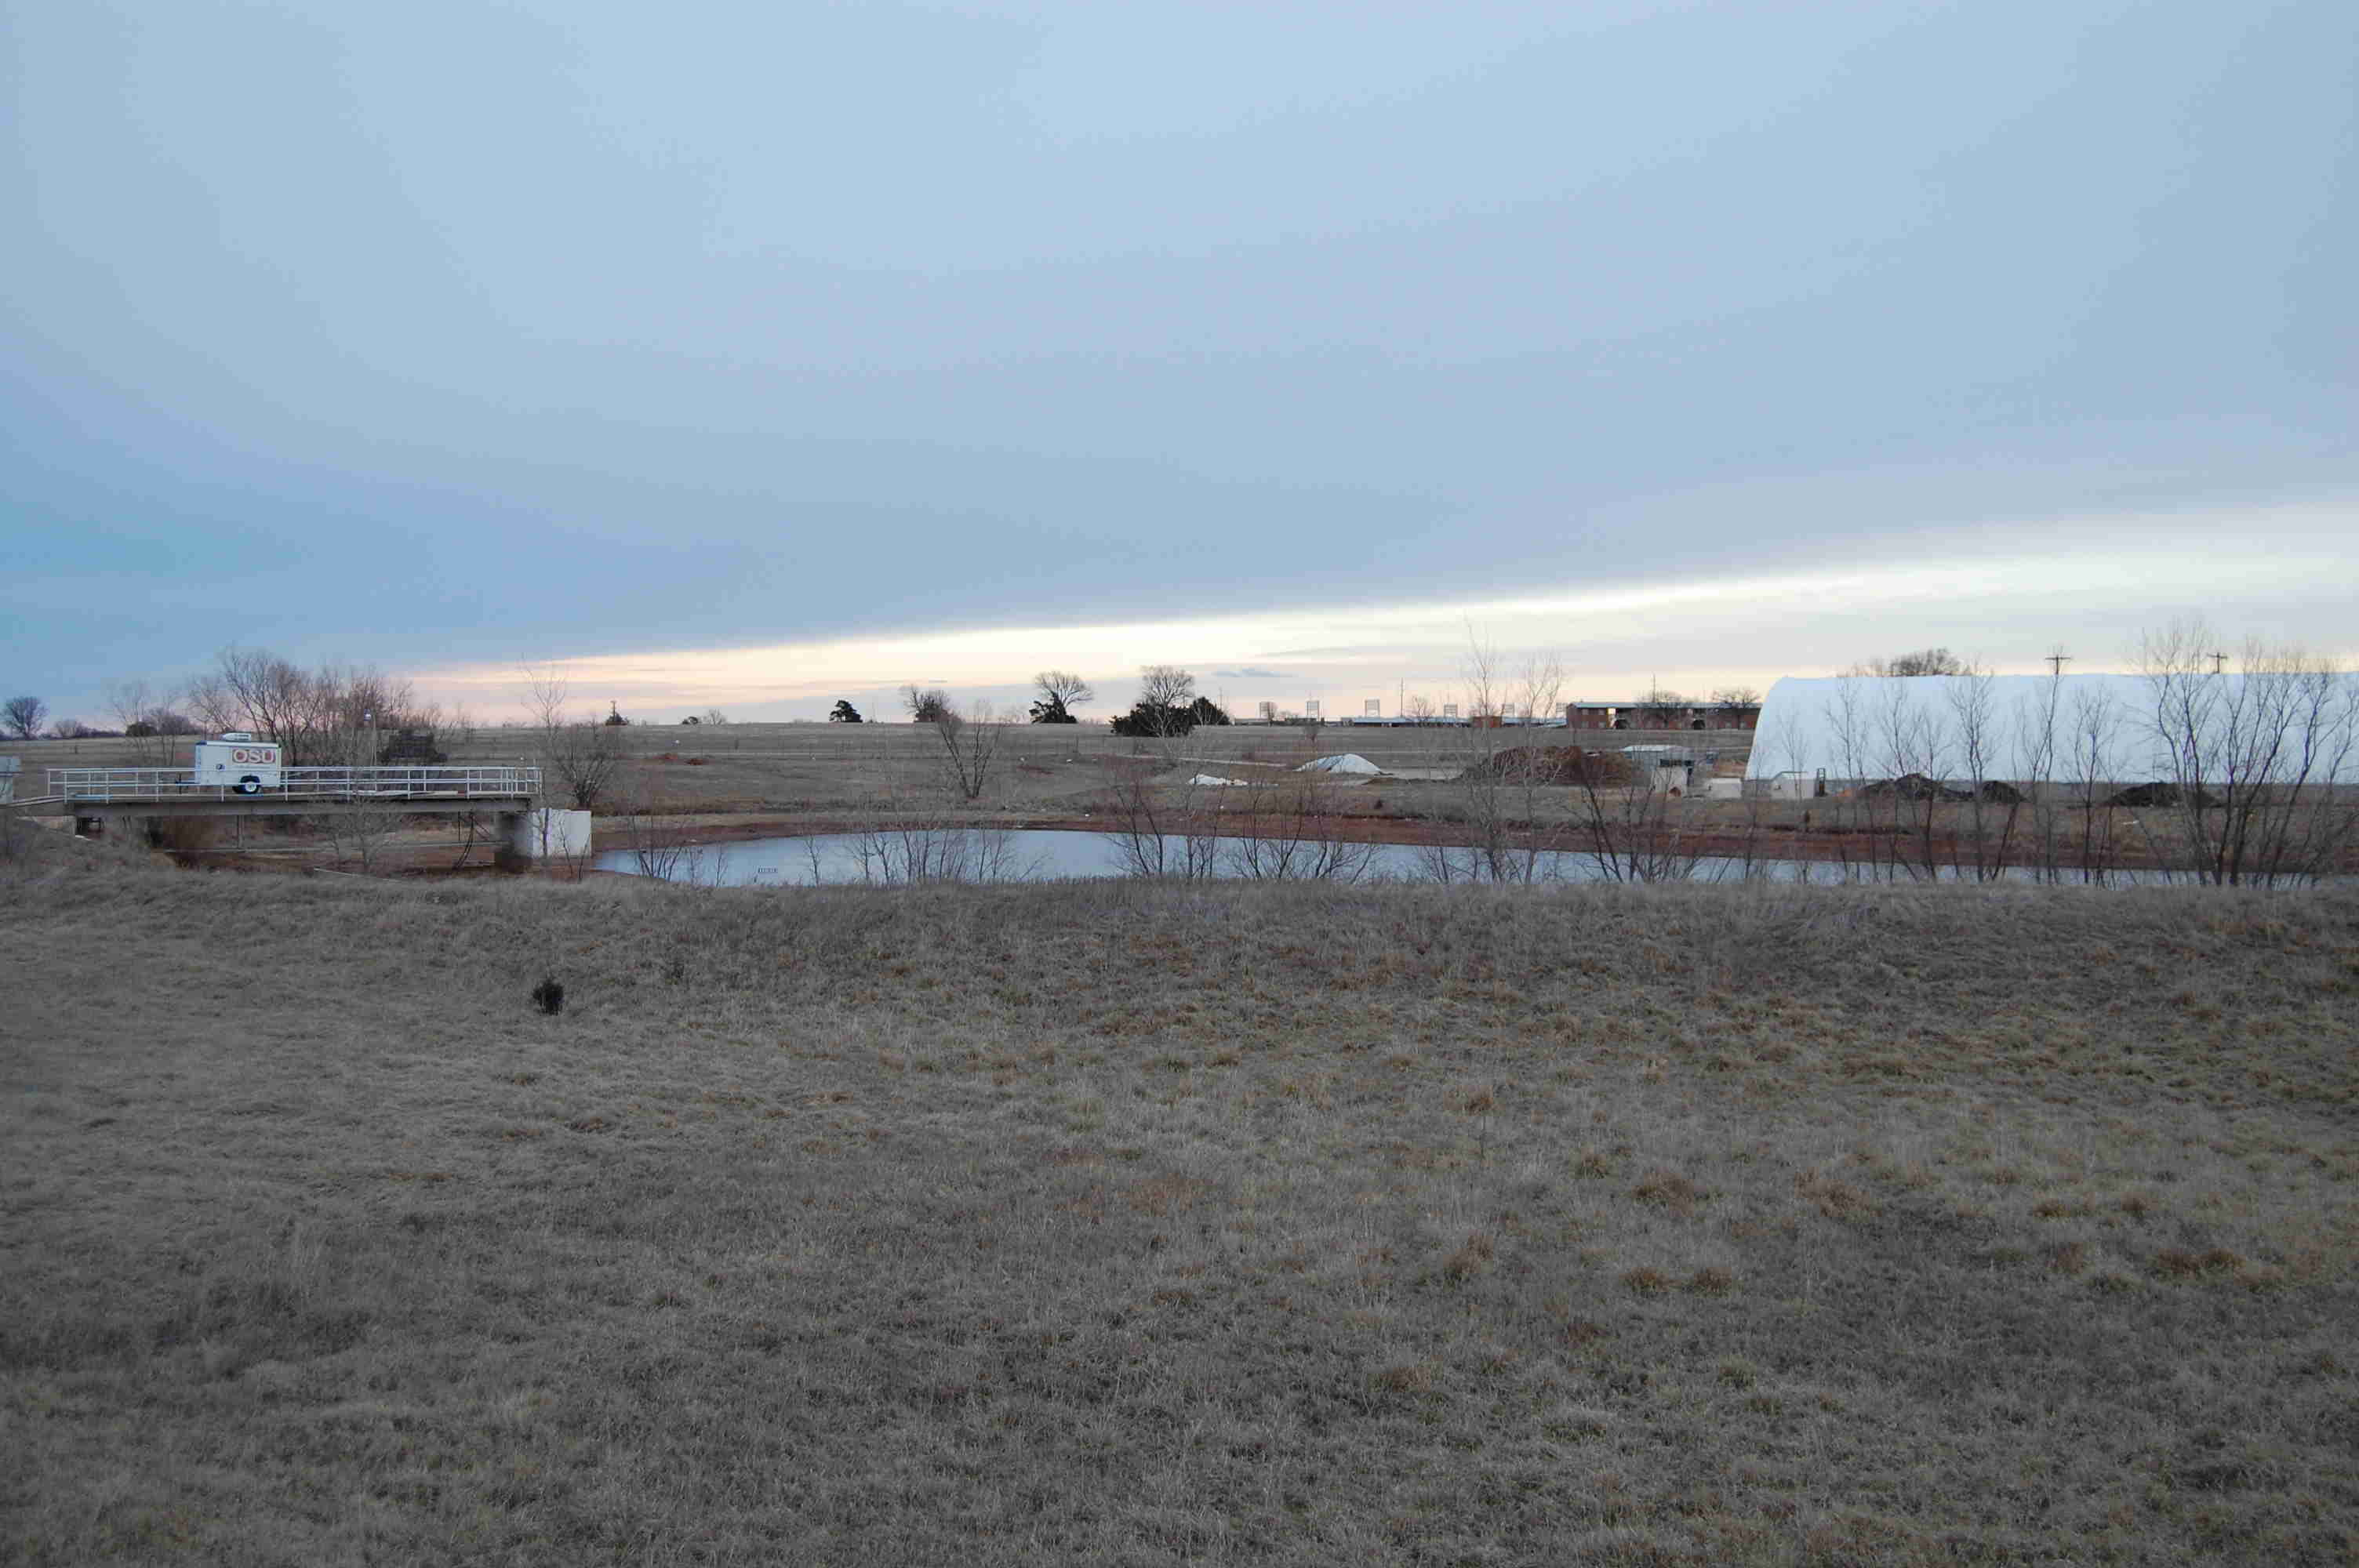
\includegraphics[width=0.47\textwidth]{Pond1.jpg}
			\label{fig:ExpMethod:HeatRej:Facility:Pond1}}
		\,
		\subfloat[View of test pond looking to the South]{
			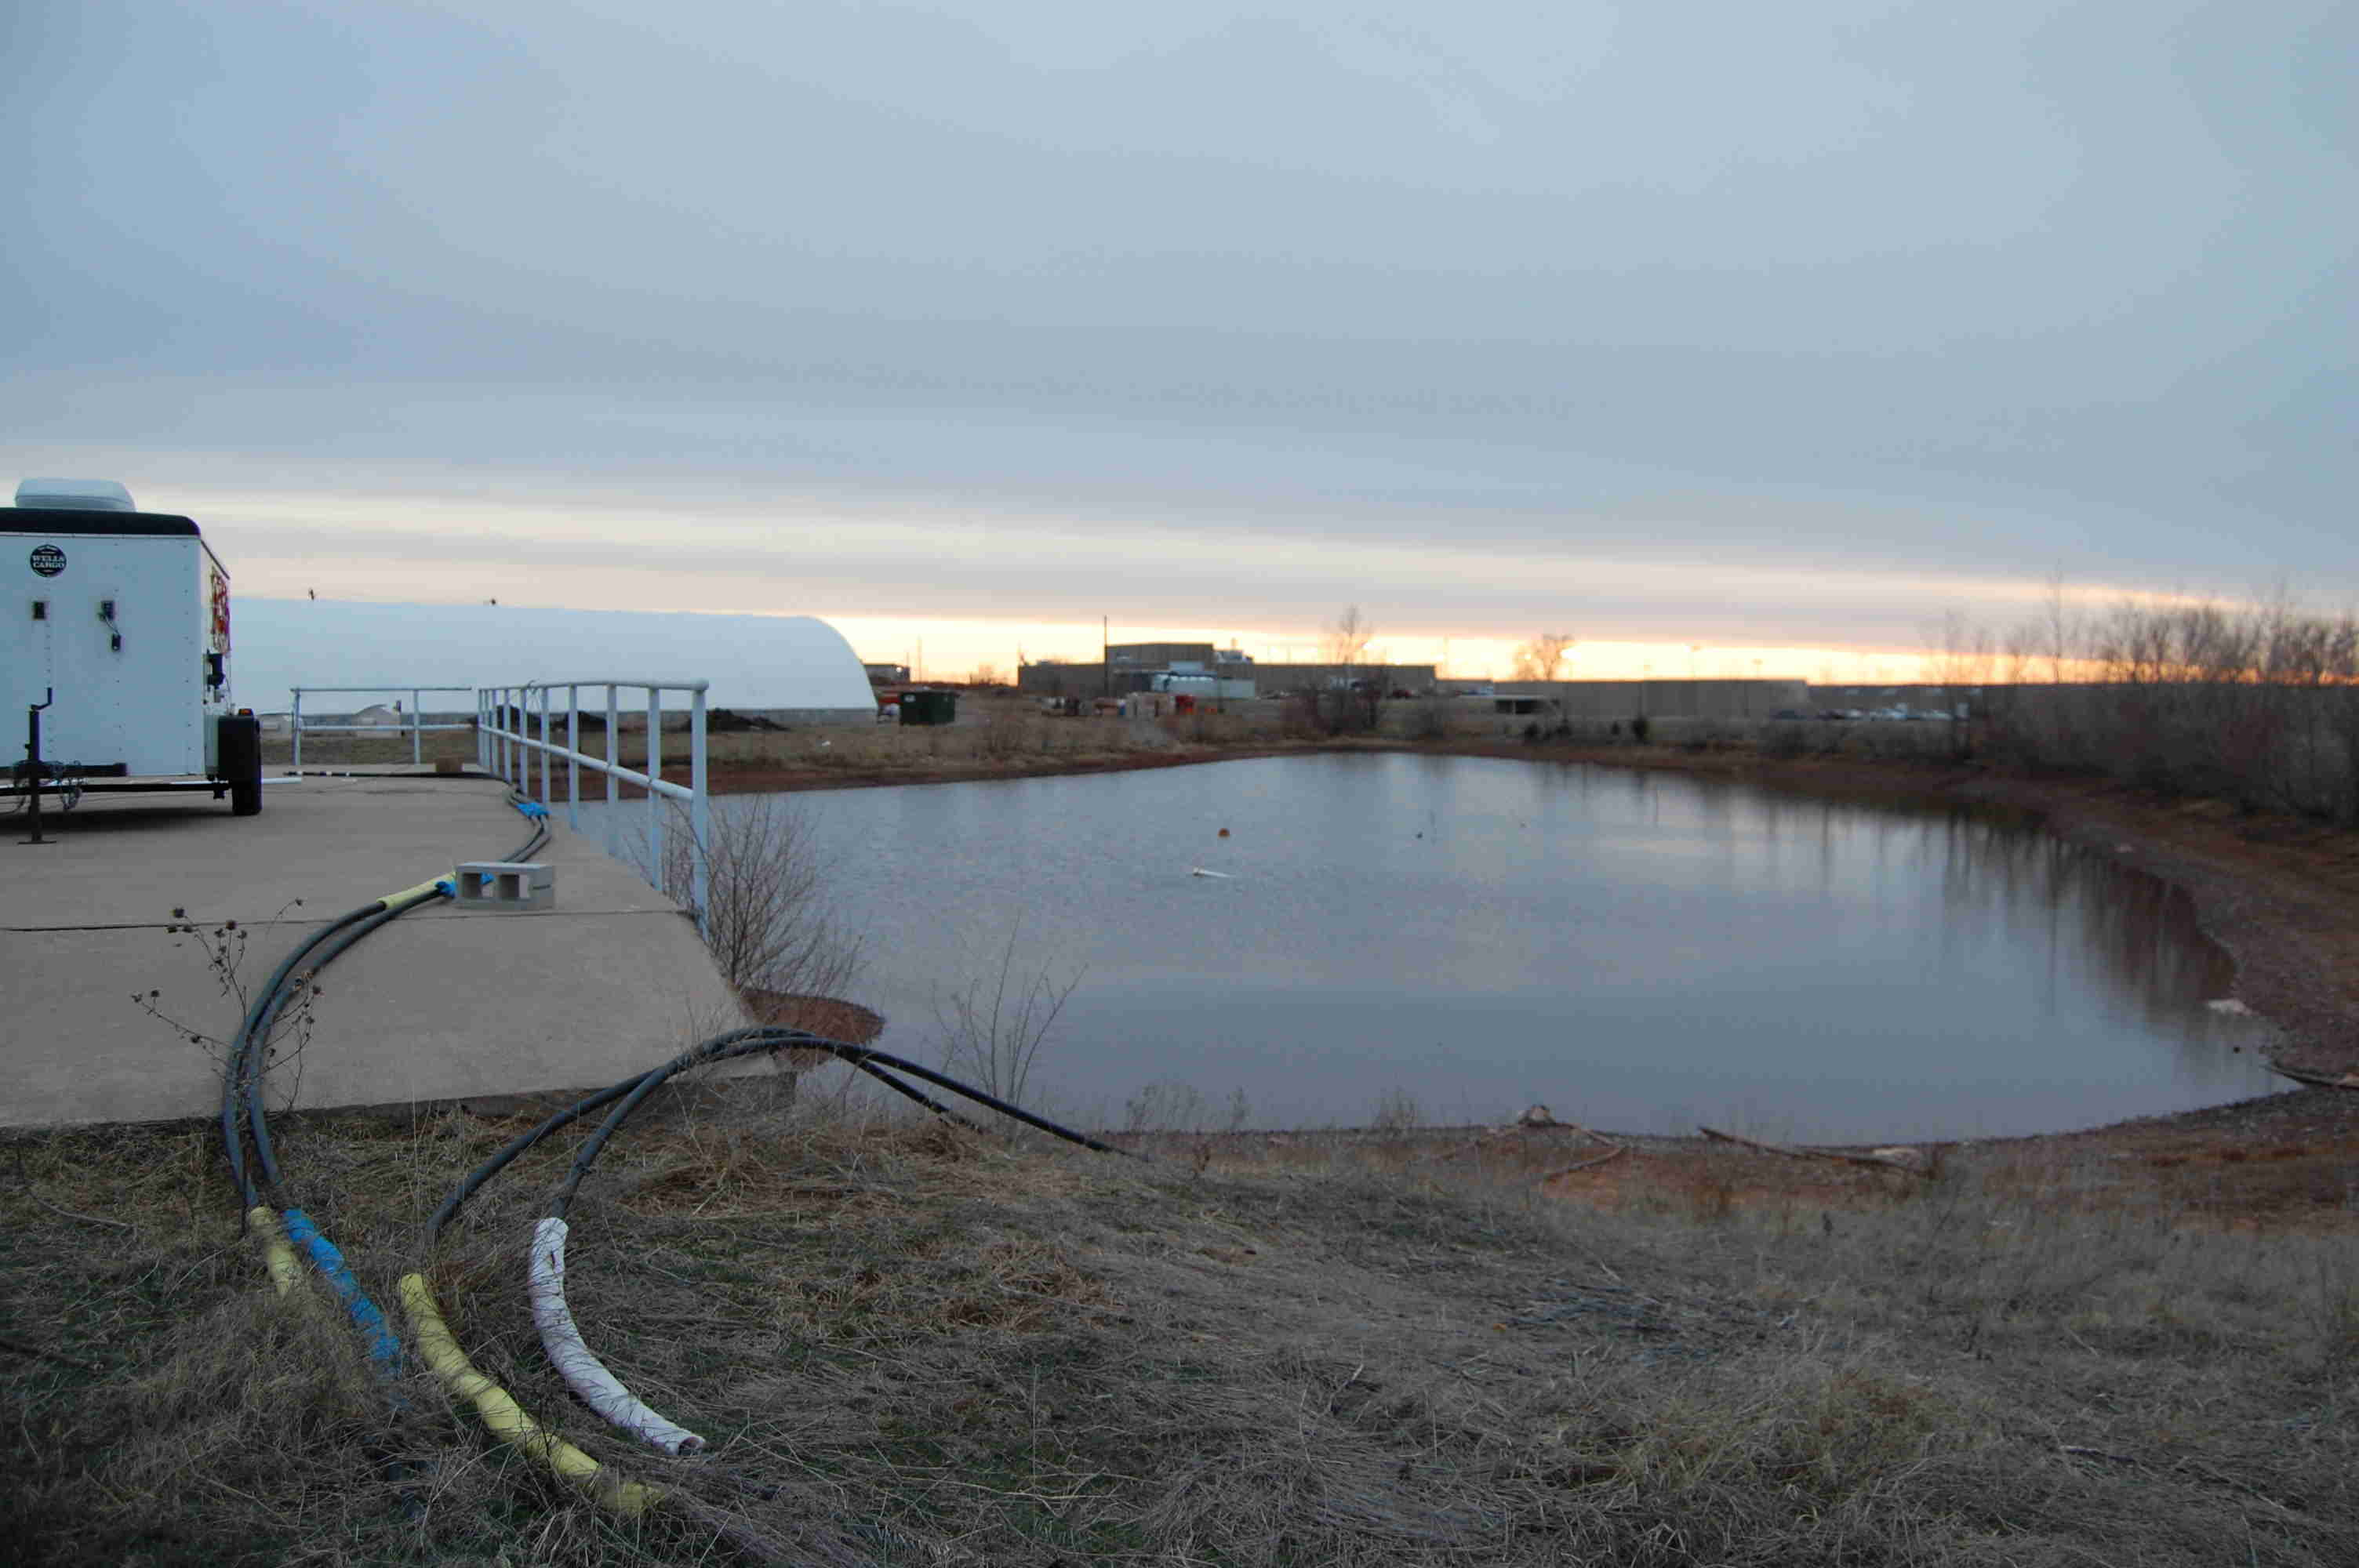
\includegraphics[width=0.47\textwidth]{Pond2.jpg}
			\label{fig:ExpMethod:HeatRej:Facility:Pond2}}
		\caption{Test pond}
		\label{fig:ExpMethod:HeatRej:Facility:PondMain}
	\end{figure}


	\begin{figure}
		\centering
		\subfloat[View of bridge deck looking to the South-east]{
			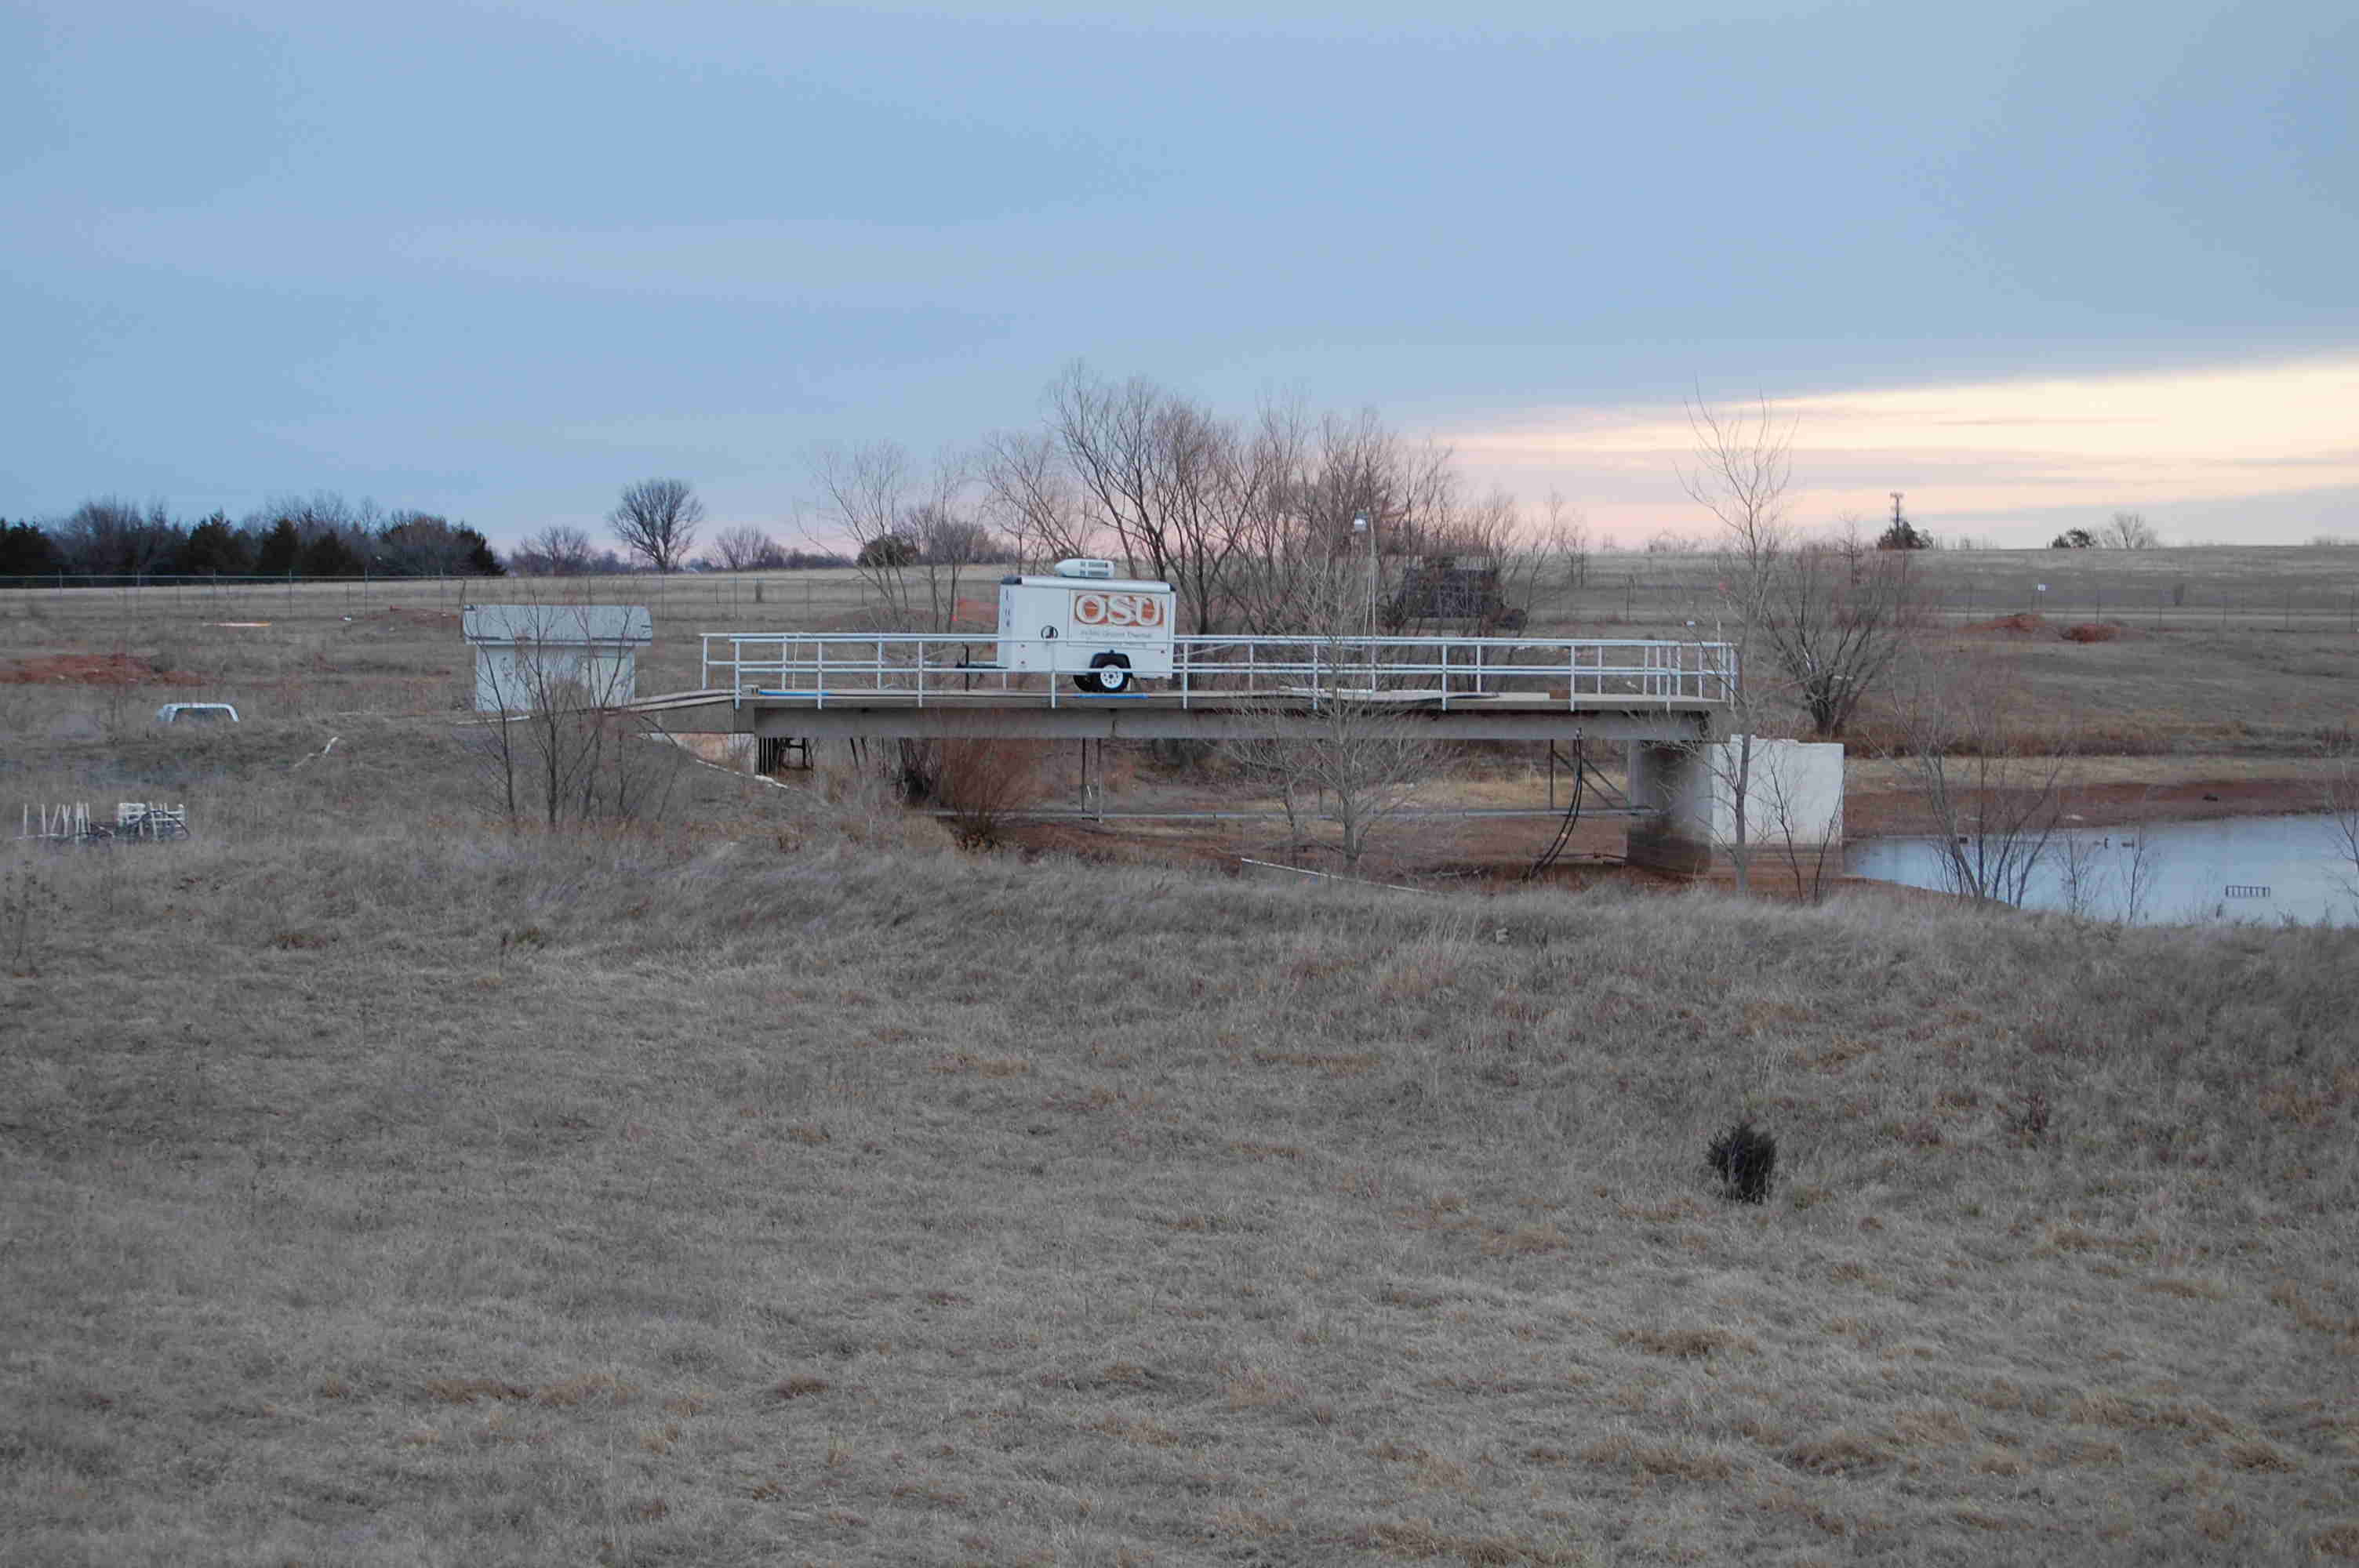
\includegraphics[width=0.47\textwidth]{Bridge1.jpg}
			\label{fig:ExpMethod:HeatRej:Facility:Bridge1}}
		\,
		\subfloat[Close view of bridge deck]{
			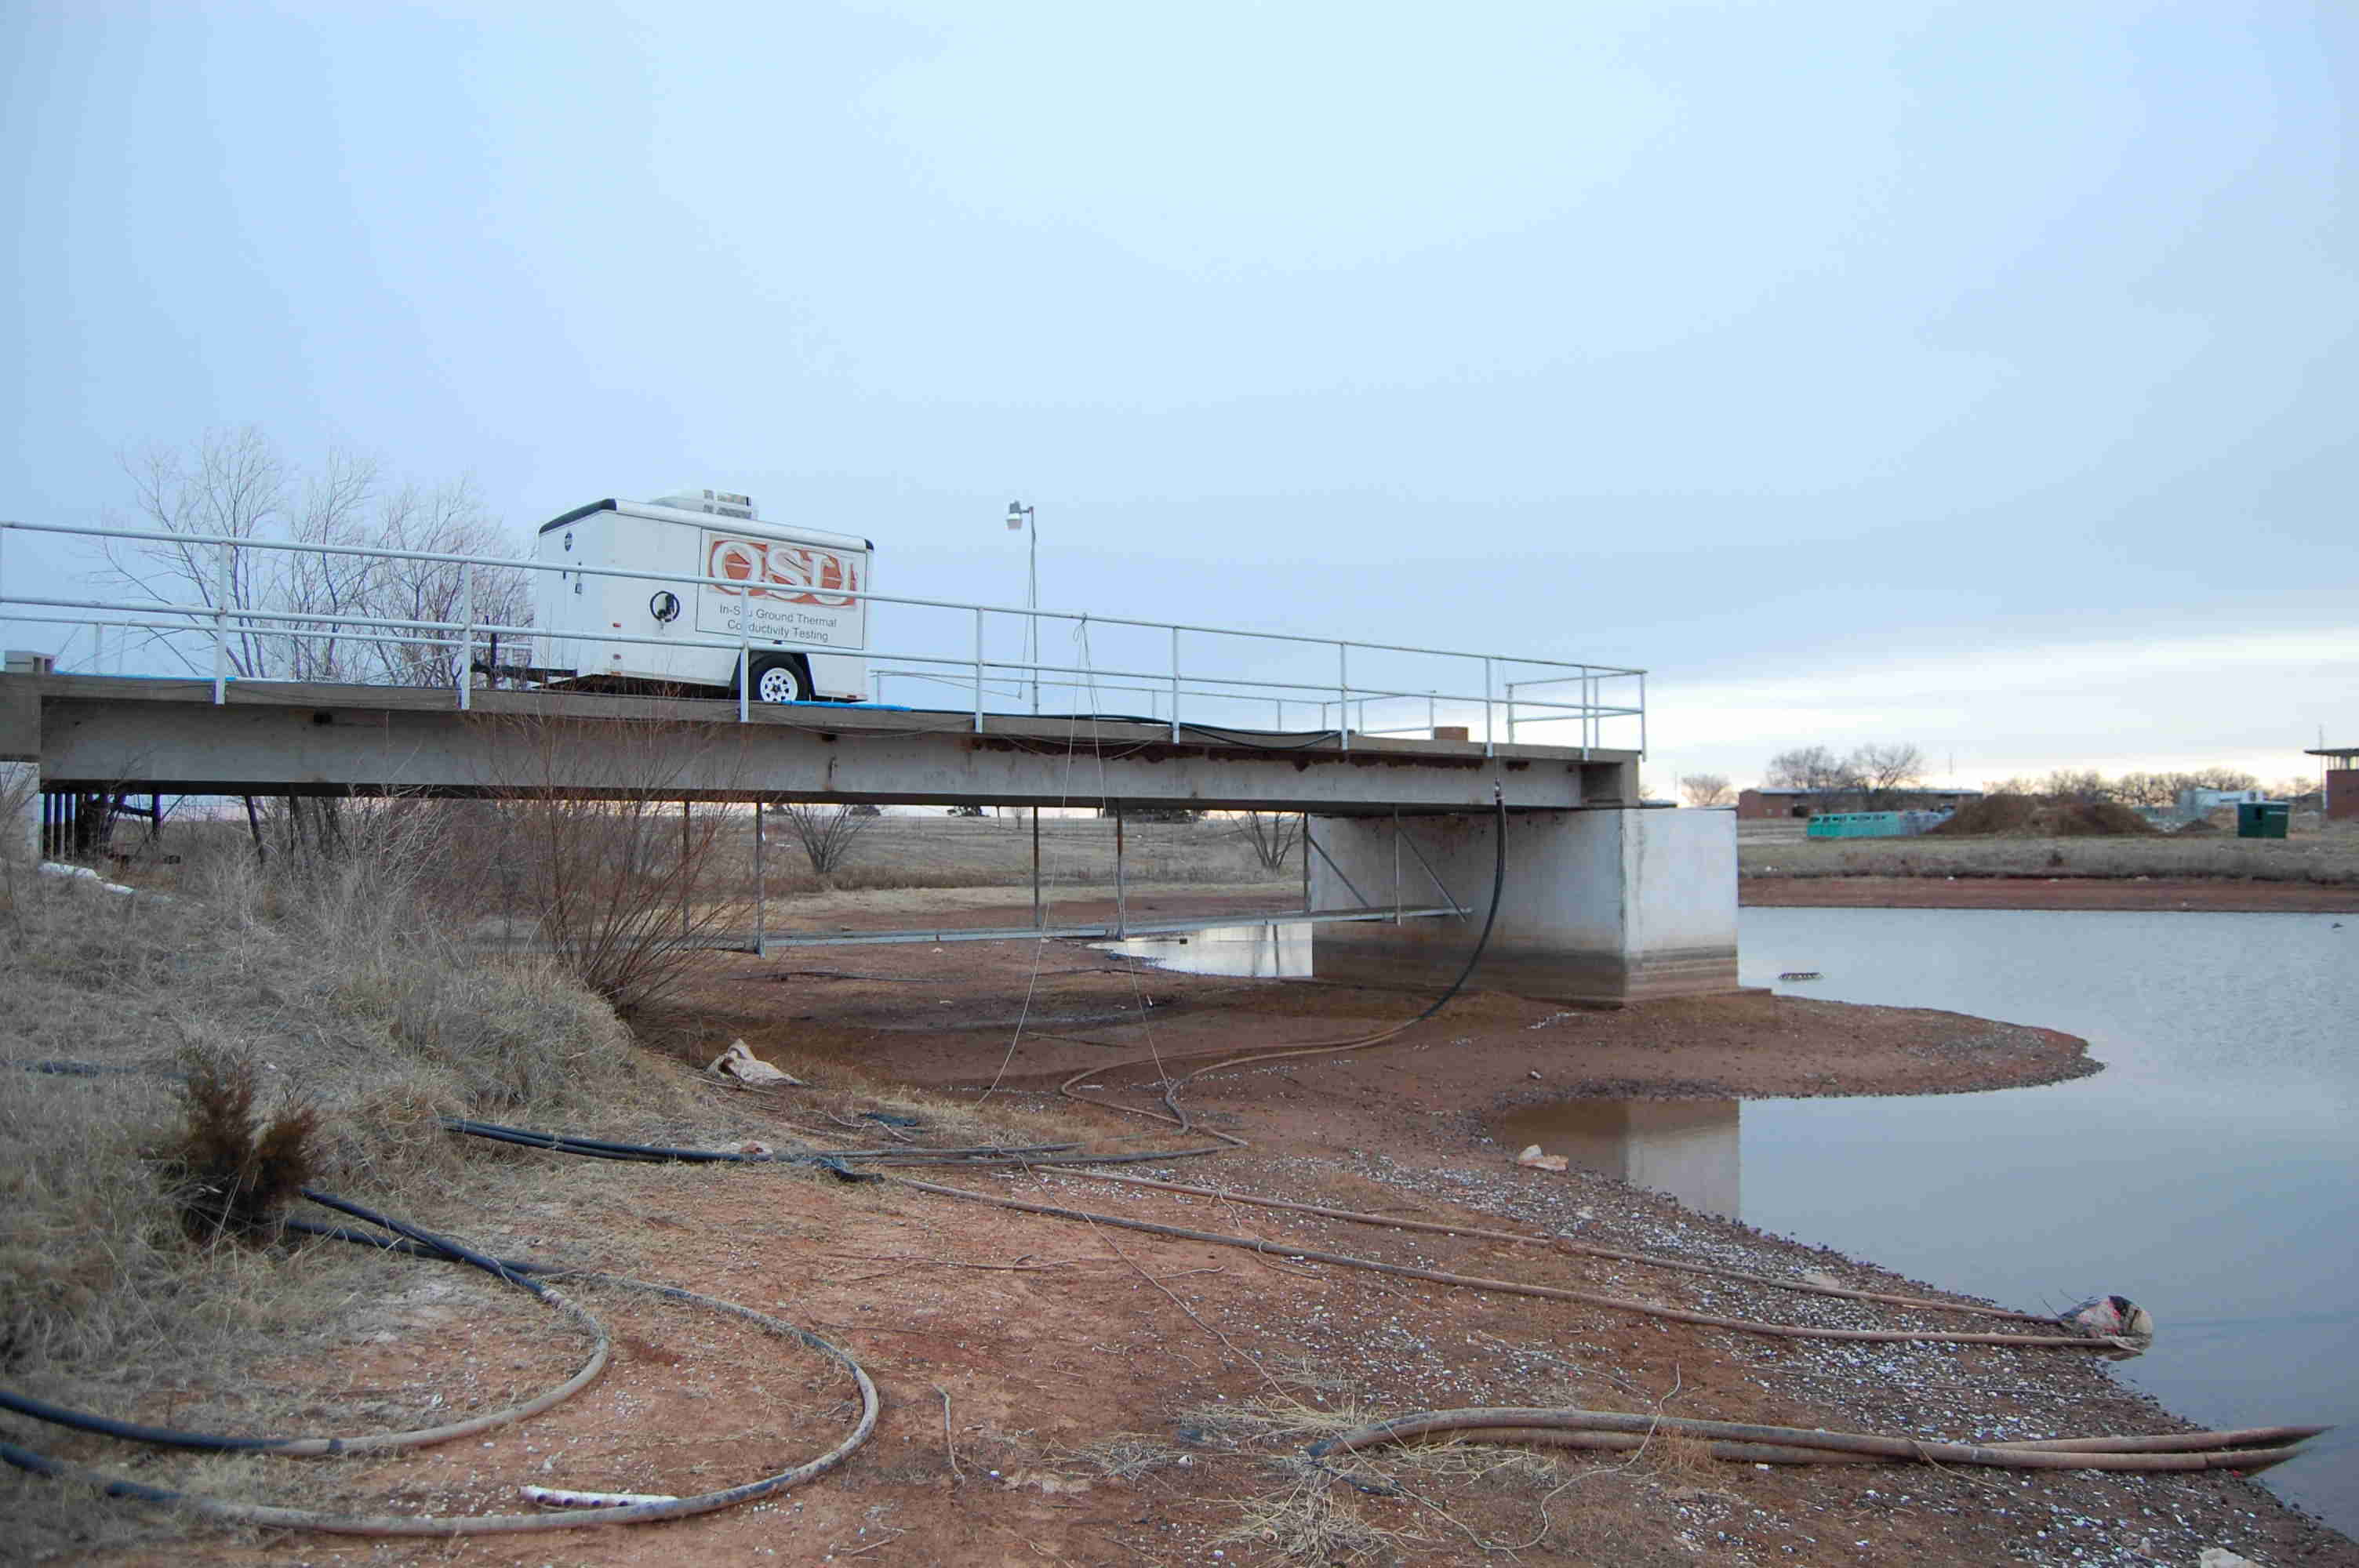
\includegraphics[width=0.47\textwidth]{Bridge2.jpg}
			\label{fig:ExpMethod:HeatRej:Facility:Bridge2}}
		\caption{Bridge deck at test pond}
		\label{fig:ExpMethod:HeatRej:Facility:BridgeMain}
	\end{figure}


	\subsection{Apparatus}
	\label{subsec:ExpMethod:HeatRej:Apparatus}

A mobile testing trailer previously utilized by \cite{Austin1998} for ground thermal conductivity testing was retrofitted for SWHE testing by \cite{Hansen2011} and was parked on the bridge deck. The mechanical and data recording equipment such as circulation pumps, flow meter, electric water heaters, valves, purge tank, purge pumps, and data loggers were all located inside the trailer situated on the bridge deck.

Figure \ref{fig:ExpMethod:HeatRej:Apparatus:RejExpTrailer} shows a schematic of the equipment and piping inside of the in-situ testing trailer used for the heat rejection tests. A photo of the equipment can be seen in Figure \ref{fig:ExpMethod:HeatRej:Apparatus:RejTrailerPic}. Once the heaters and the SWHE were purged of air, the 3-way valves were oriented so that the fluid circulated in a closed loop. The circulating fluid would then cascade across three electrical resistance heaters arranged in series and dissipate the heat via the SWHE.

	\begin{figure}
		\centering
		\subfloat[Schematic of heat rejection equipment in trailer.]{
			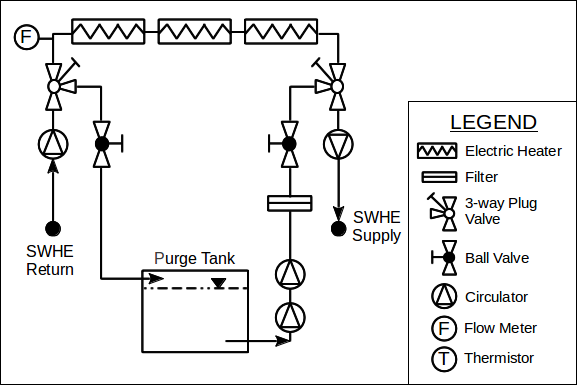
\includegraphics[width=0.47\textwidth]{Exp_Setup_Rejection.png}
			\label{fig:ExpMethod:HeatRej:Apparatus:RejExpTrailer}}
		\,
		\subfloat[Equipment inside heat rejection trailer. \textit{Reprinted, by permission, from \cite{Hansen2011}}]{
			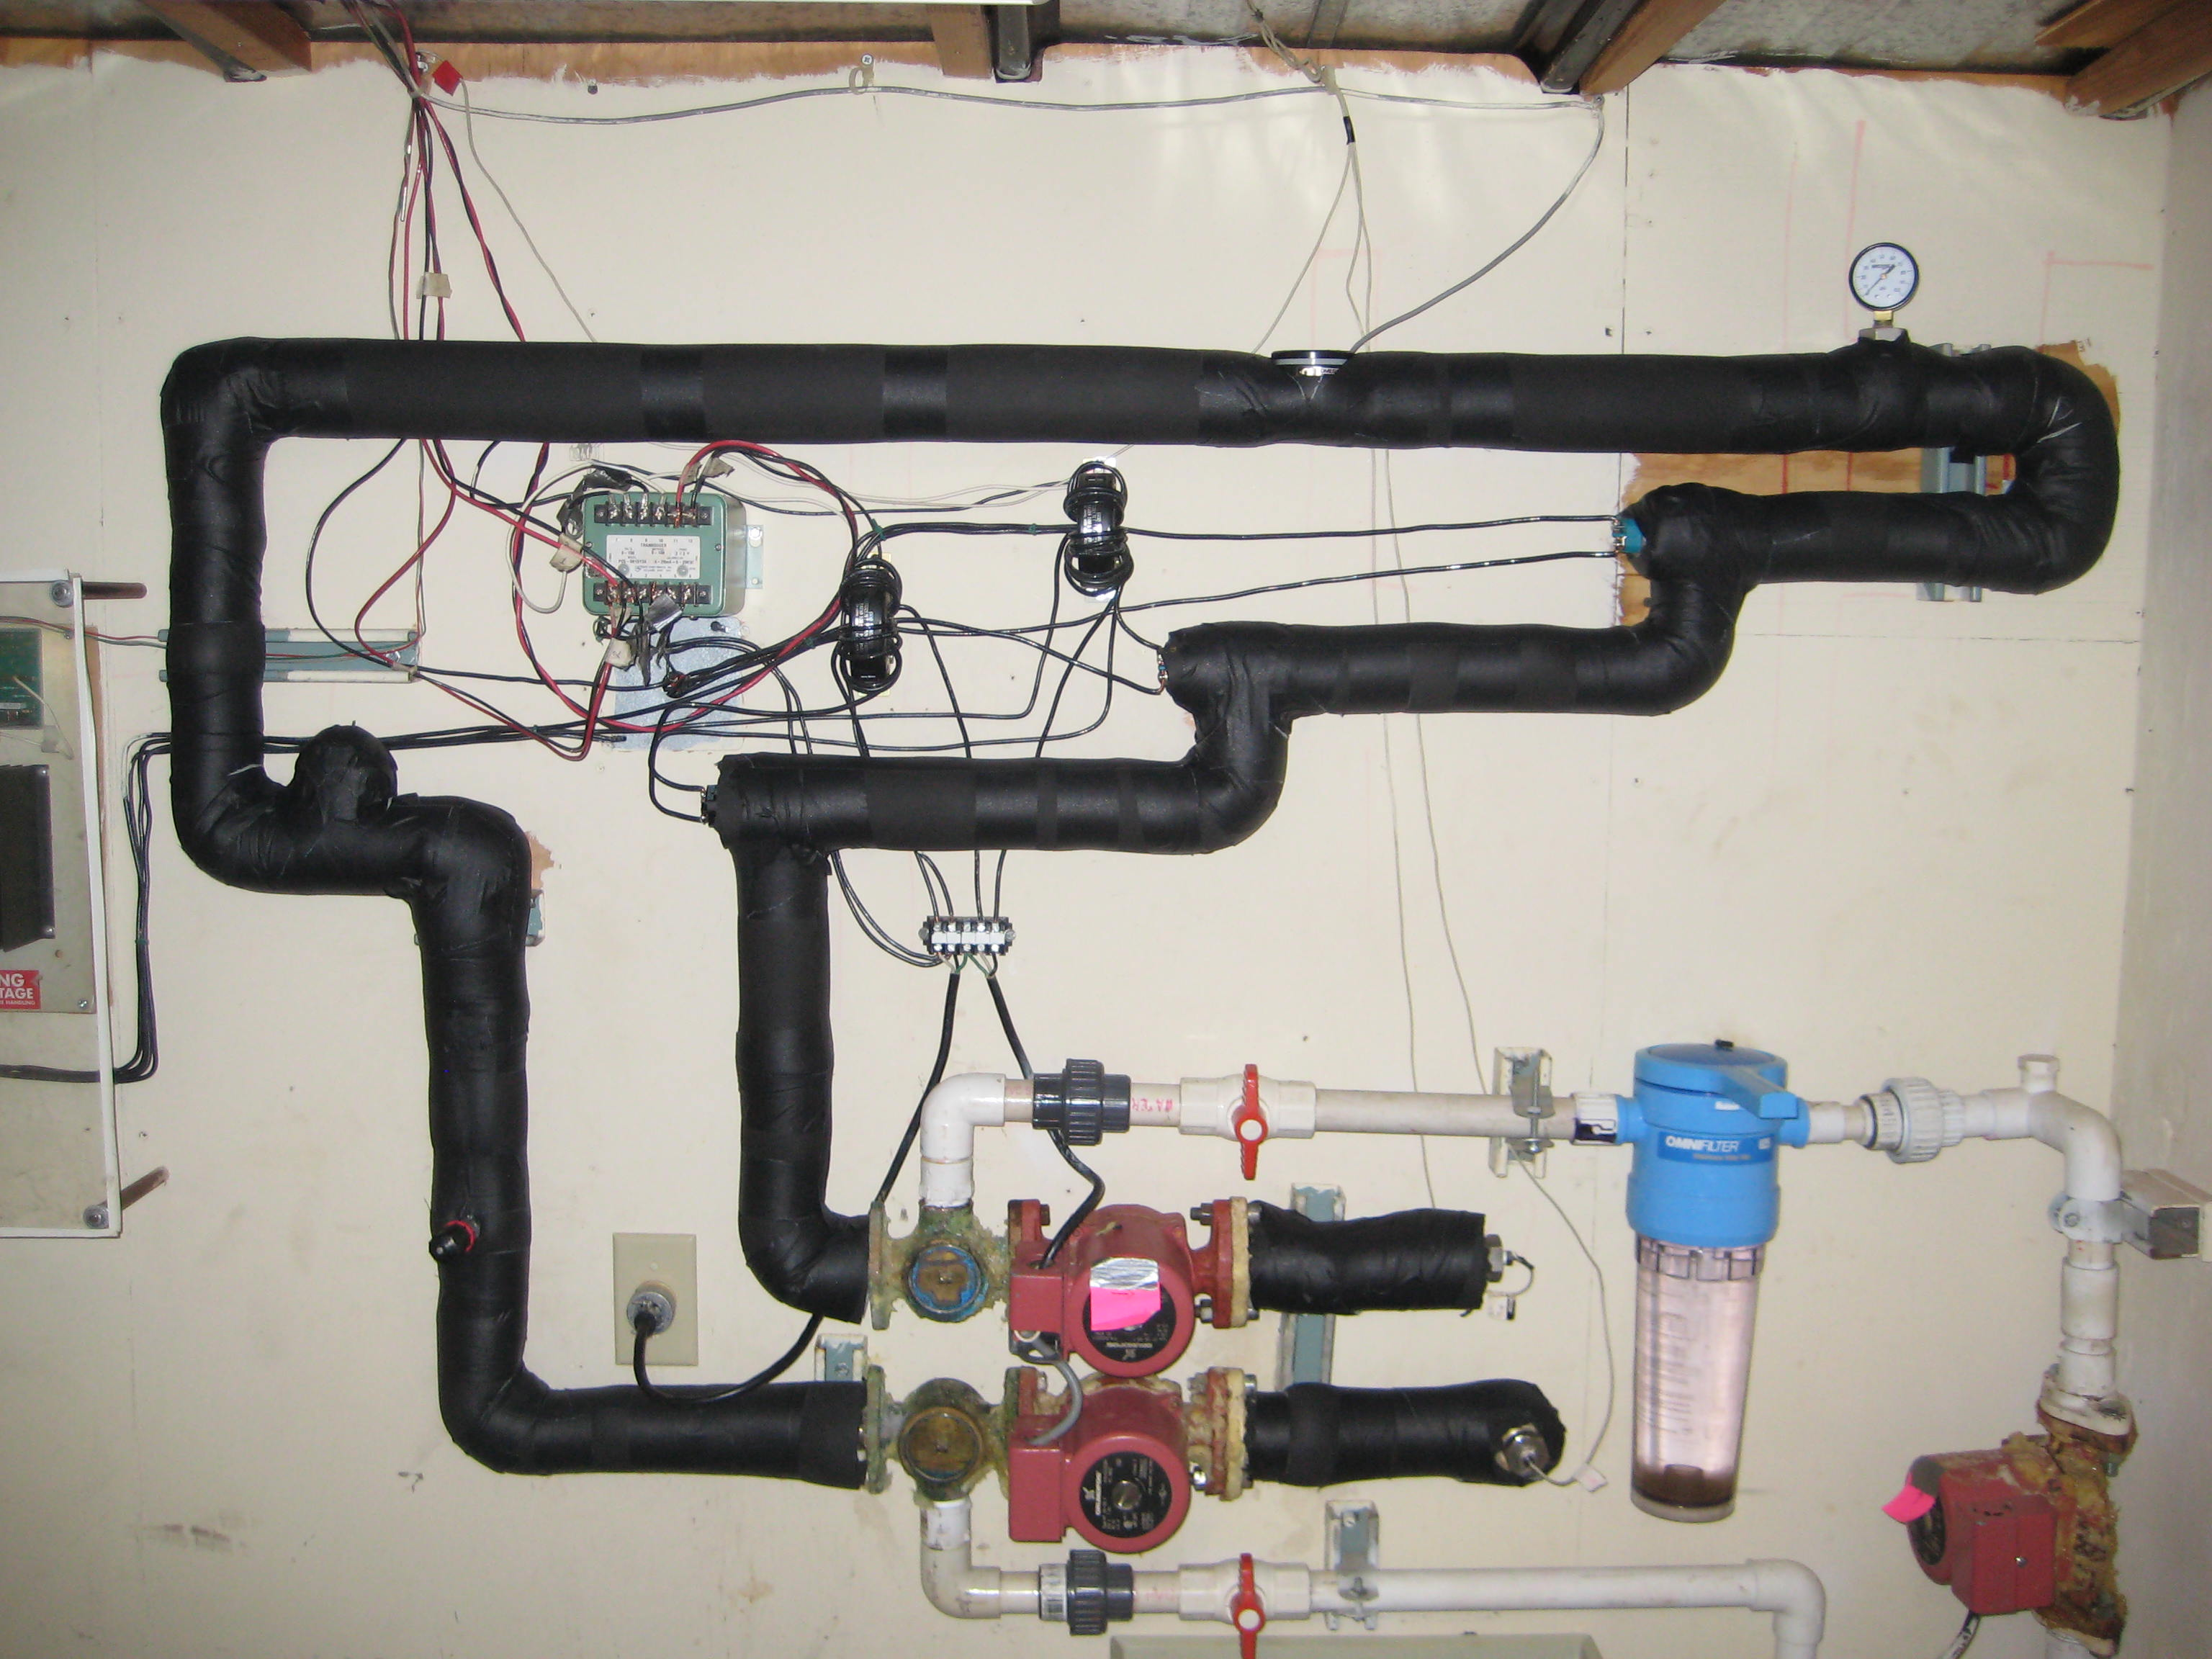
\includegraphics[width=0.47\textwidth]{Rej_Trailer.jpg}
			\label{fig:ExpMethod:HeatRej:Apparatus:RejTrailerPic}}
		\caption[Heat rejection trailer equipment]{Heat rejection trailer equipment}
		\label{fig:ExpMethod:HeatRej:Apparatus:RejTrailer}
	\end{figure}

The SWHE was placed on a support frame and then placed in the pond. The support frame was supported from the water surface by buoys. This method of supporting the SWHE from the water surface allowed the depth of the SWHE to be controlled accurately. It also allowed the SWHE depth relative to the water surface to remain at a fixed distance. On hot summer days in Oklahoma, the test pond depth could drop one-half to one inch (12-25 mm) each day due to evaporation. Supporting the SWHE from the water surface using buoys allowed the SWHE to remain a fixed distance from the water surface at all times. The SWHE was also anchored in place in the pond to prevent wind or underwater currents from causing the SWHE to move in the pond. A schematic of the SWHE in the pond can be seen in Figure \ref{fig:ExpMethod:HeatRej:Apparatus:RejExpPond}.

Figure \ref{fig:ExpMethod:HeatRej:Apparatus:ExtrCoil} and shows a spiral-helical coil on land prepared for testing while Figure  \ref{fig:ExpMethod:HeatRej:Apparatus:ExtrCoilInPond} shows the coil in place in the pond during a test. Also visible in Figure \ref{fig:ExpMethod:HeatRej:Apparatus:ExtrCoilInPond},  are three vertical tubes which were placed on the coil support frame $120^\circ$ apart from each other. The bottom of the tubes were placed at the bottom of the SWHE, and from there were marked at the submersion depth. This provided a visual means by which the depth of the coil could be verified which would occur once the marks were even with the water surface.

The flow rate was measured by a calibrated turbine flow meter. In-pipe thermistors were placed at the inlet and outlet of the SWHE to measure entering and exiting fluid temperatures. An in-pipe thermistor can be seen in Figure \ref{fig:ExpMethod:HeatRej:Apparatus:InPipeThermistor}. The pond temperature was also measured at the bottom, middle, and top of the coil at a distance of 4 ft.\ (1.2 m)  away from the SWHE. The L-arm attached to the SWHE coil frame can be seen Figure \ref{fig:ExpMethod:HeatRej:Apparatus:LArm} and is where the local thermistors were placed in order to measure the local pond water temperature. The pond temperature was averaged from the three temperature measurements to determine the lake temperature. This is shown in Equation \ref{eq:ExpMethod:HeatRej:Apparatus:PondTemp}.

\begin{equation}
	T_{sw} = \frac{T_{top} + 2 \cdot T_{mid} + T_{bot}}{4}
	\label{eq:ExpMethod:HeatRej:Apparatus:PondTemp}
\end{equation}



	\begin{figure}
		\centering
		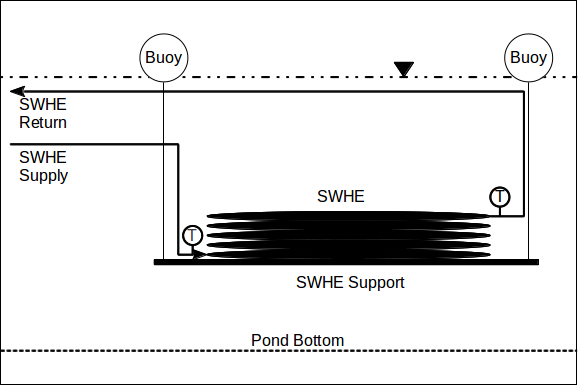
\includegraphics[width=0.8\textwidth]{SWHE_Rej_Pond.png}
		\caption[Schematic of heat rejection experiment in pond]{Schematic of heat rejection experiment in pond}
		\label{fig:ExpMethod:HeatRej:Apparatus:RejExpPond}
	\end{figure}

	\begin{figure}
		\centering
		\subfloat[Spiral-helical surface water heat exchanger prepared for testing.]{
			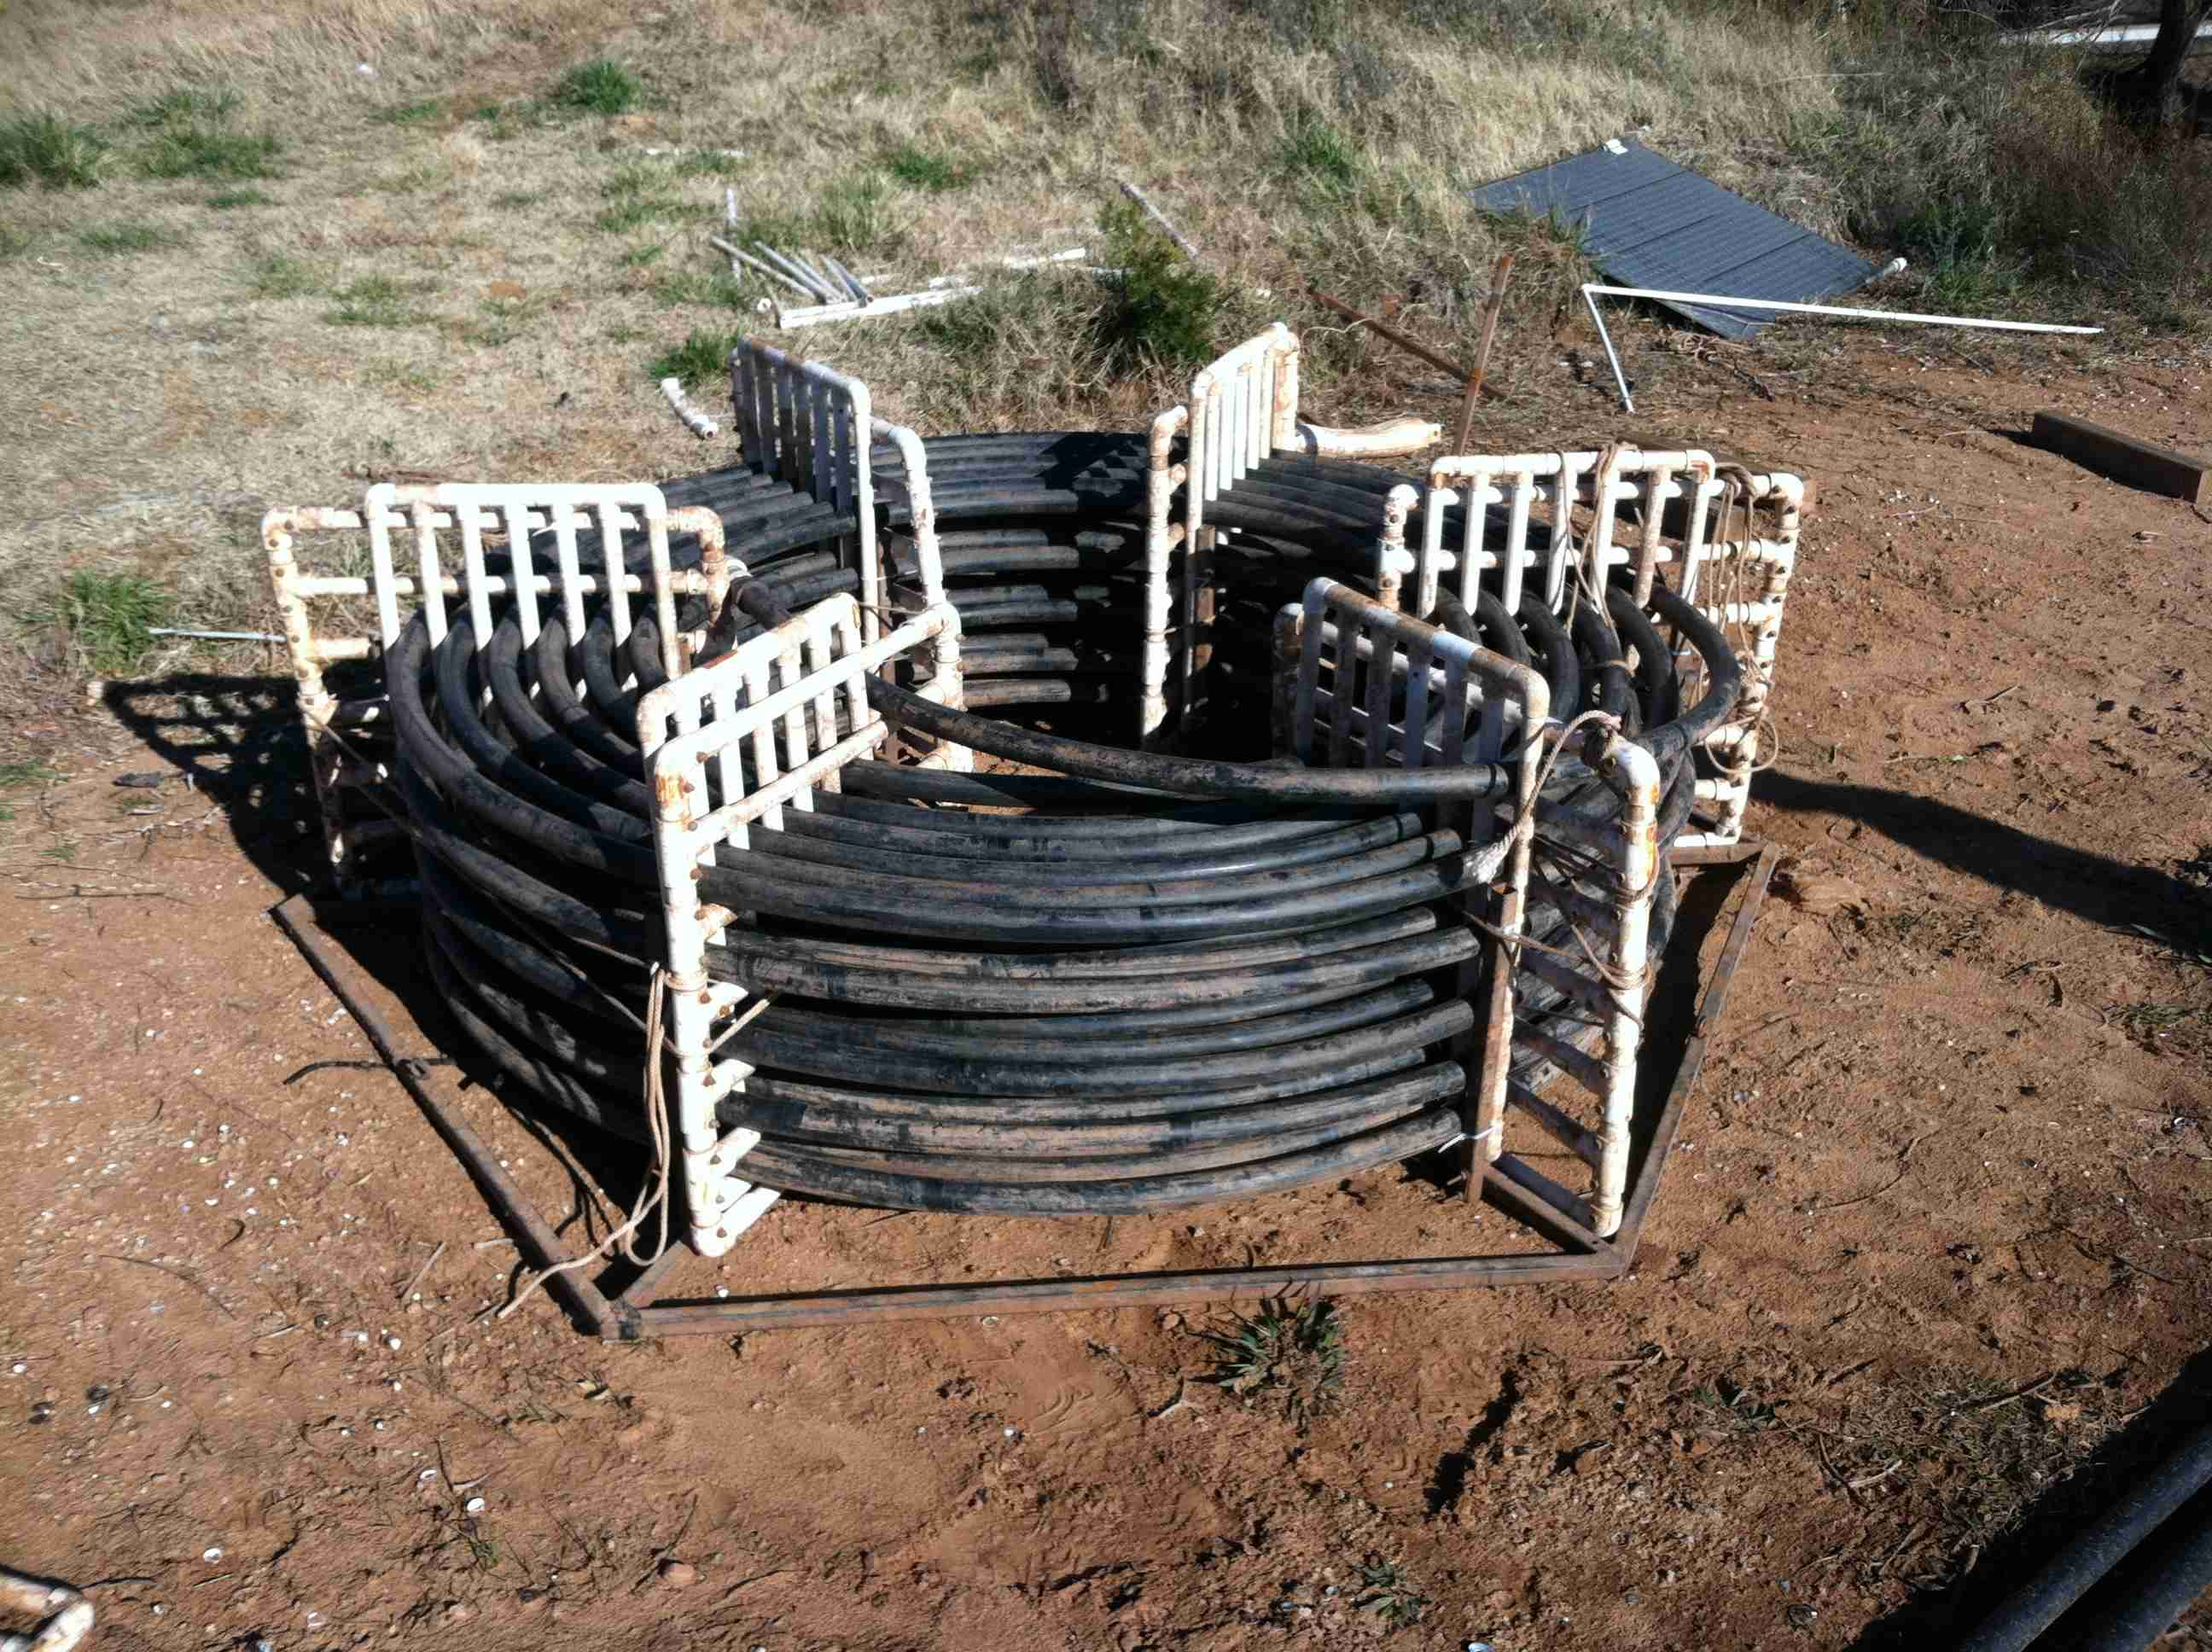
\includegraphics[width=0.47\textwidth]{Extr_Coil.jpg}
			\label{fig:ExpMethod:HeatRej:Apparatus:ExtrCoil}}
		\,
		\subfloat[Coil in test pond during test.]{
			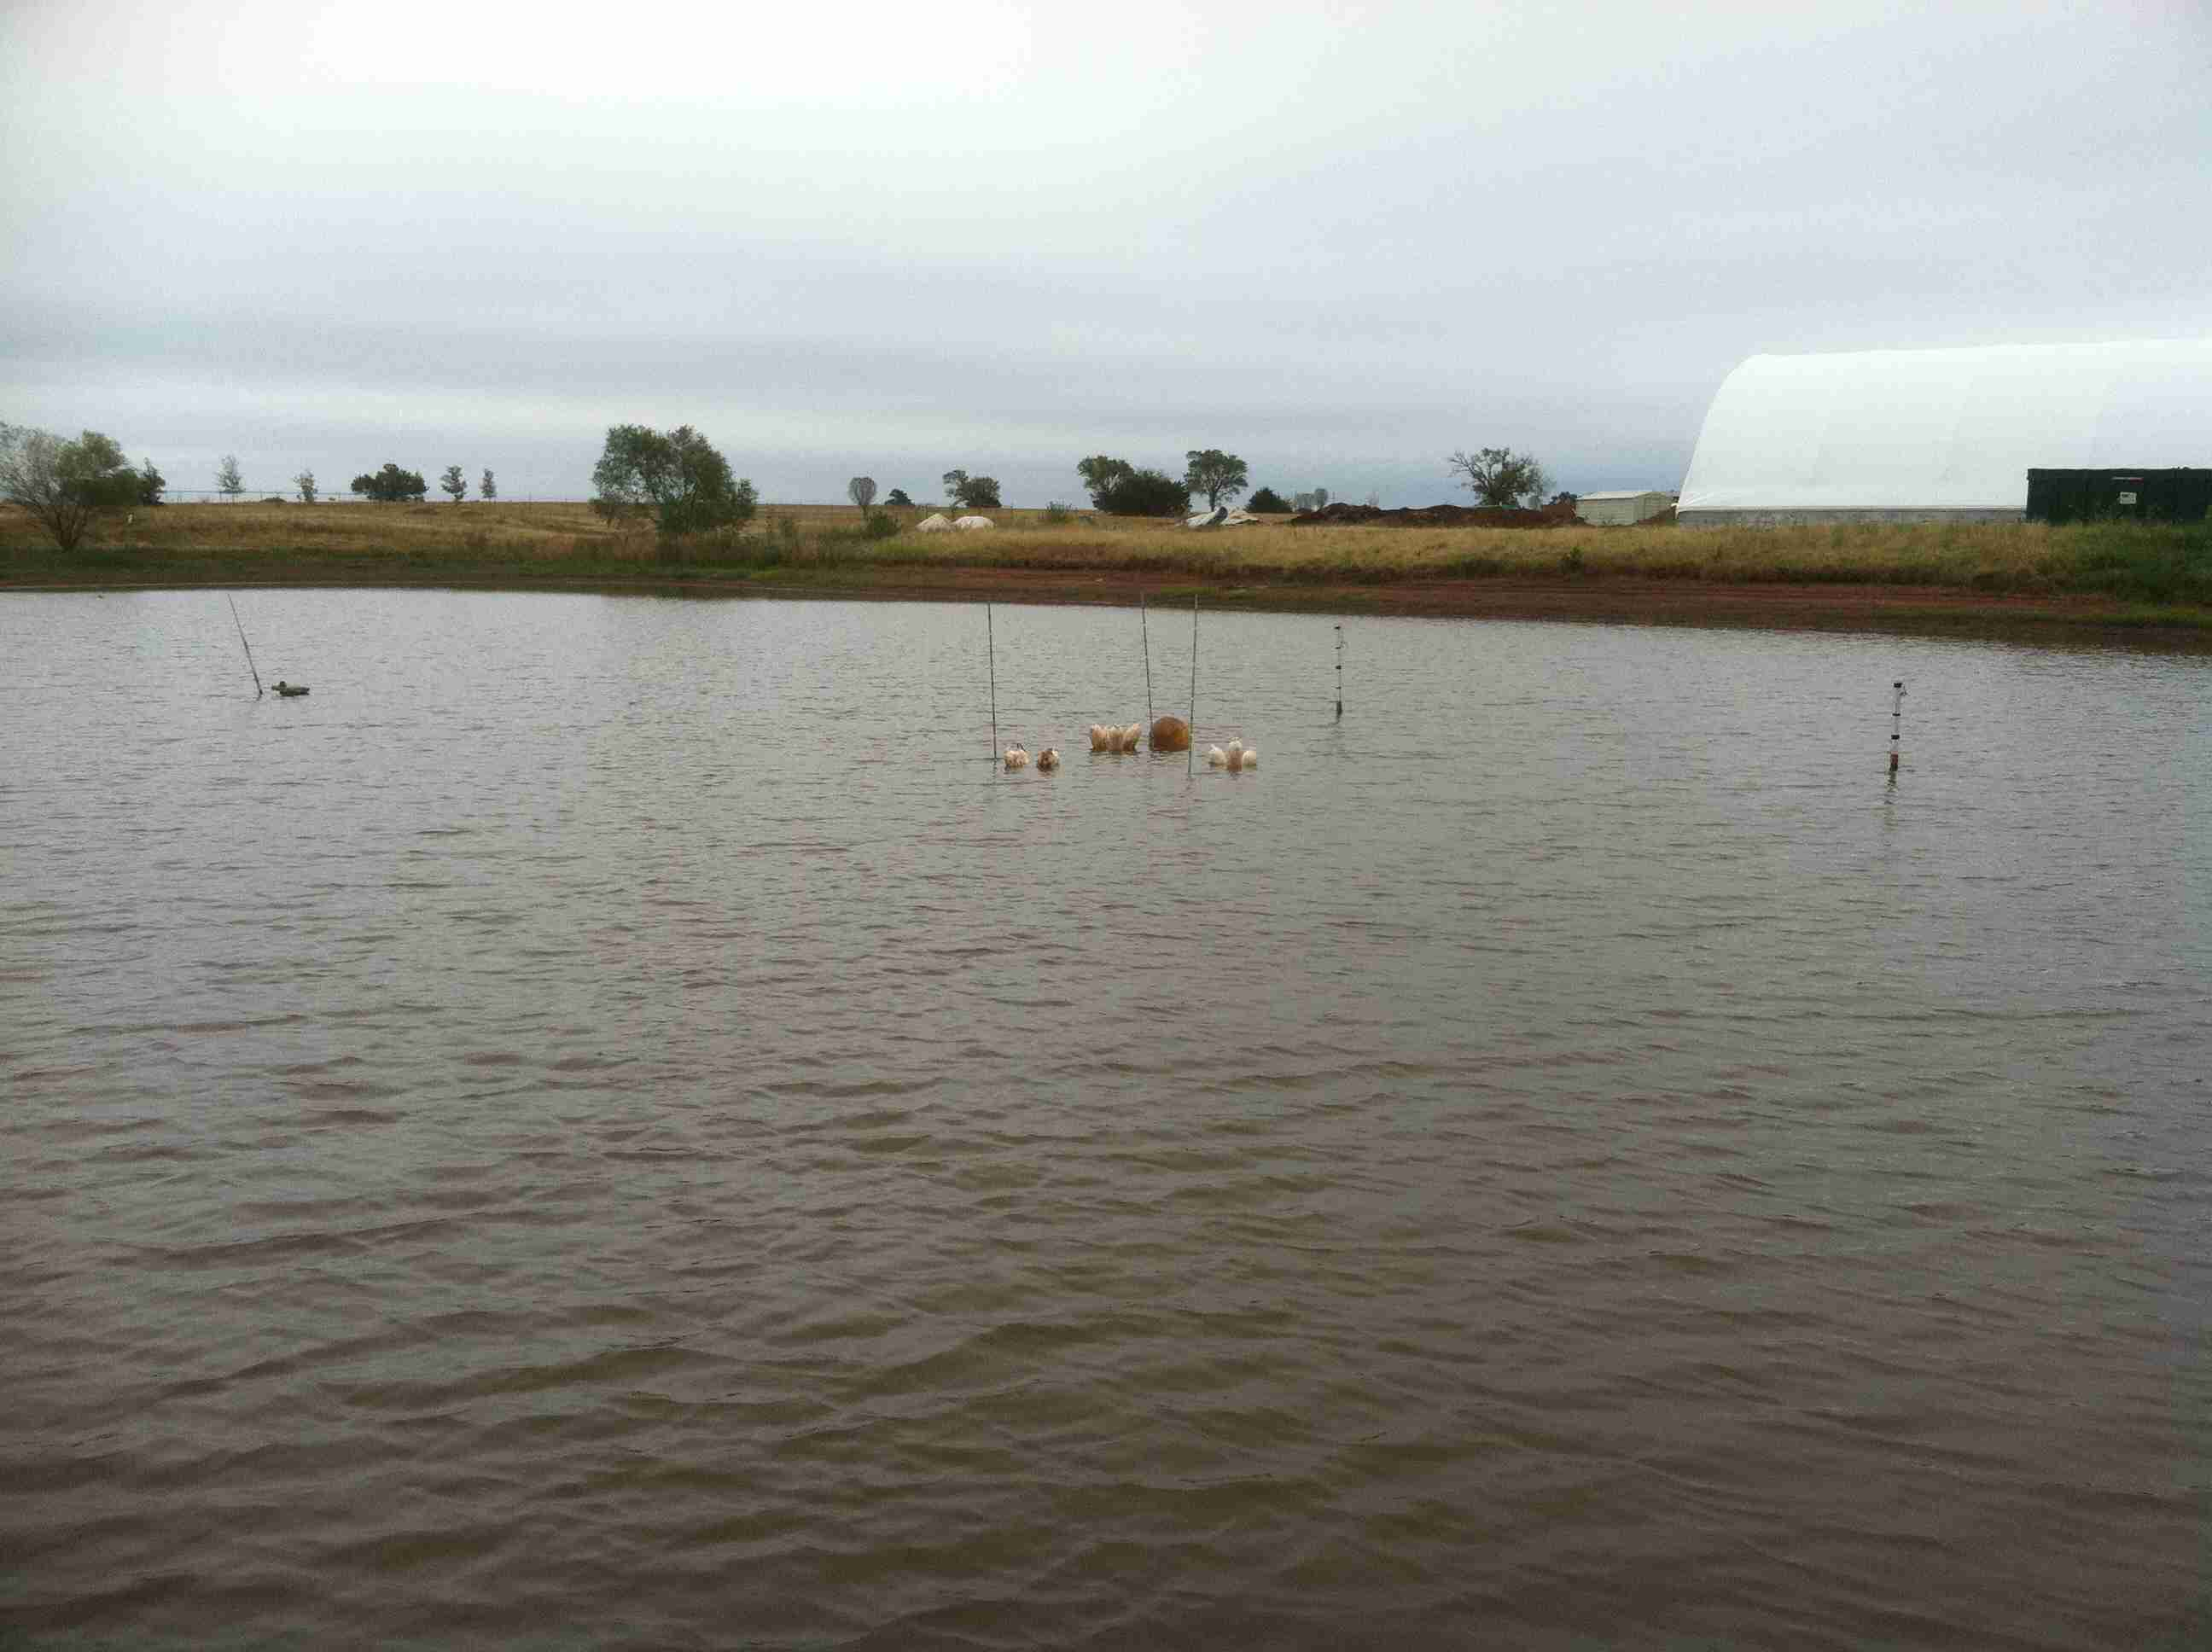
\includegraphics[width=0.47\textwidth]{Coil_In_Pond.jpg}
			\label{fig:ExpMethod:HeatRej:Apparatus:ExtrCoilInPond}}
		\caption[Surface water heat exchanger]{Surface water heat exchanger}
		\label{fig:ExpMethod:HeatRej:Apparatus:RejCoilInPond}
	\end{figure}


	\begin{figure}
		\centering
		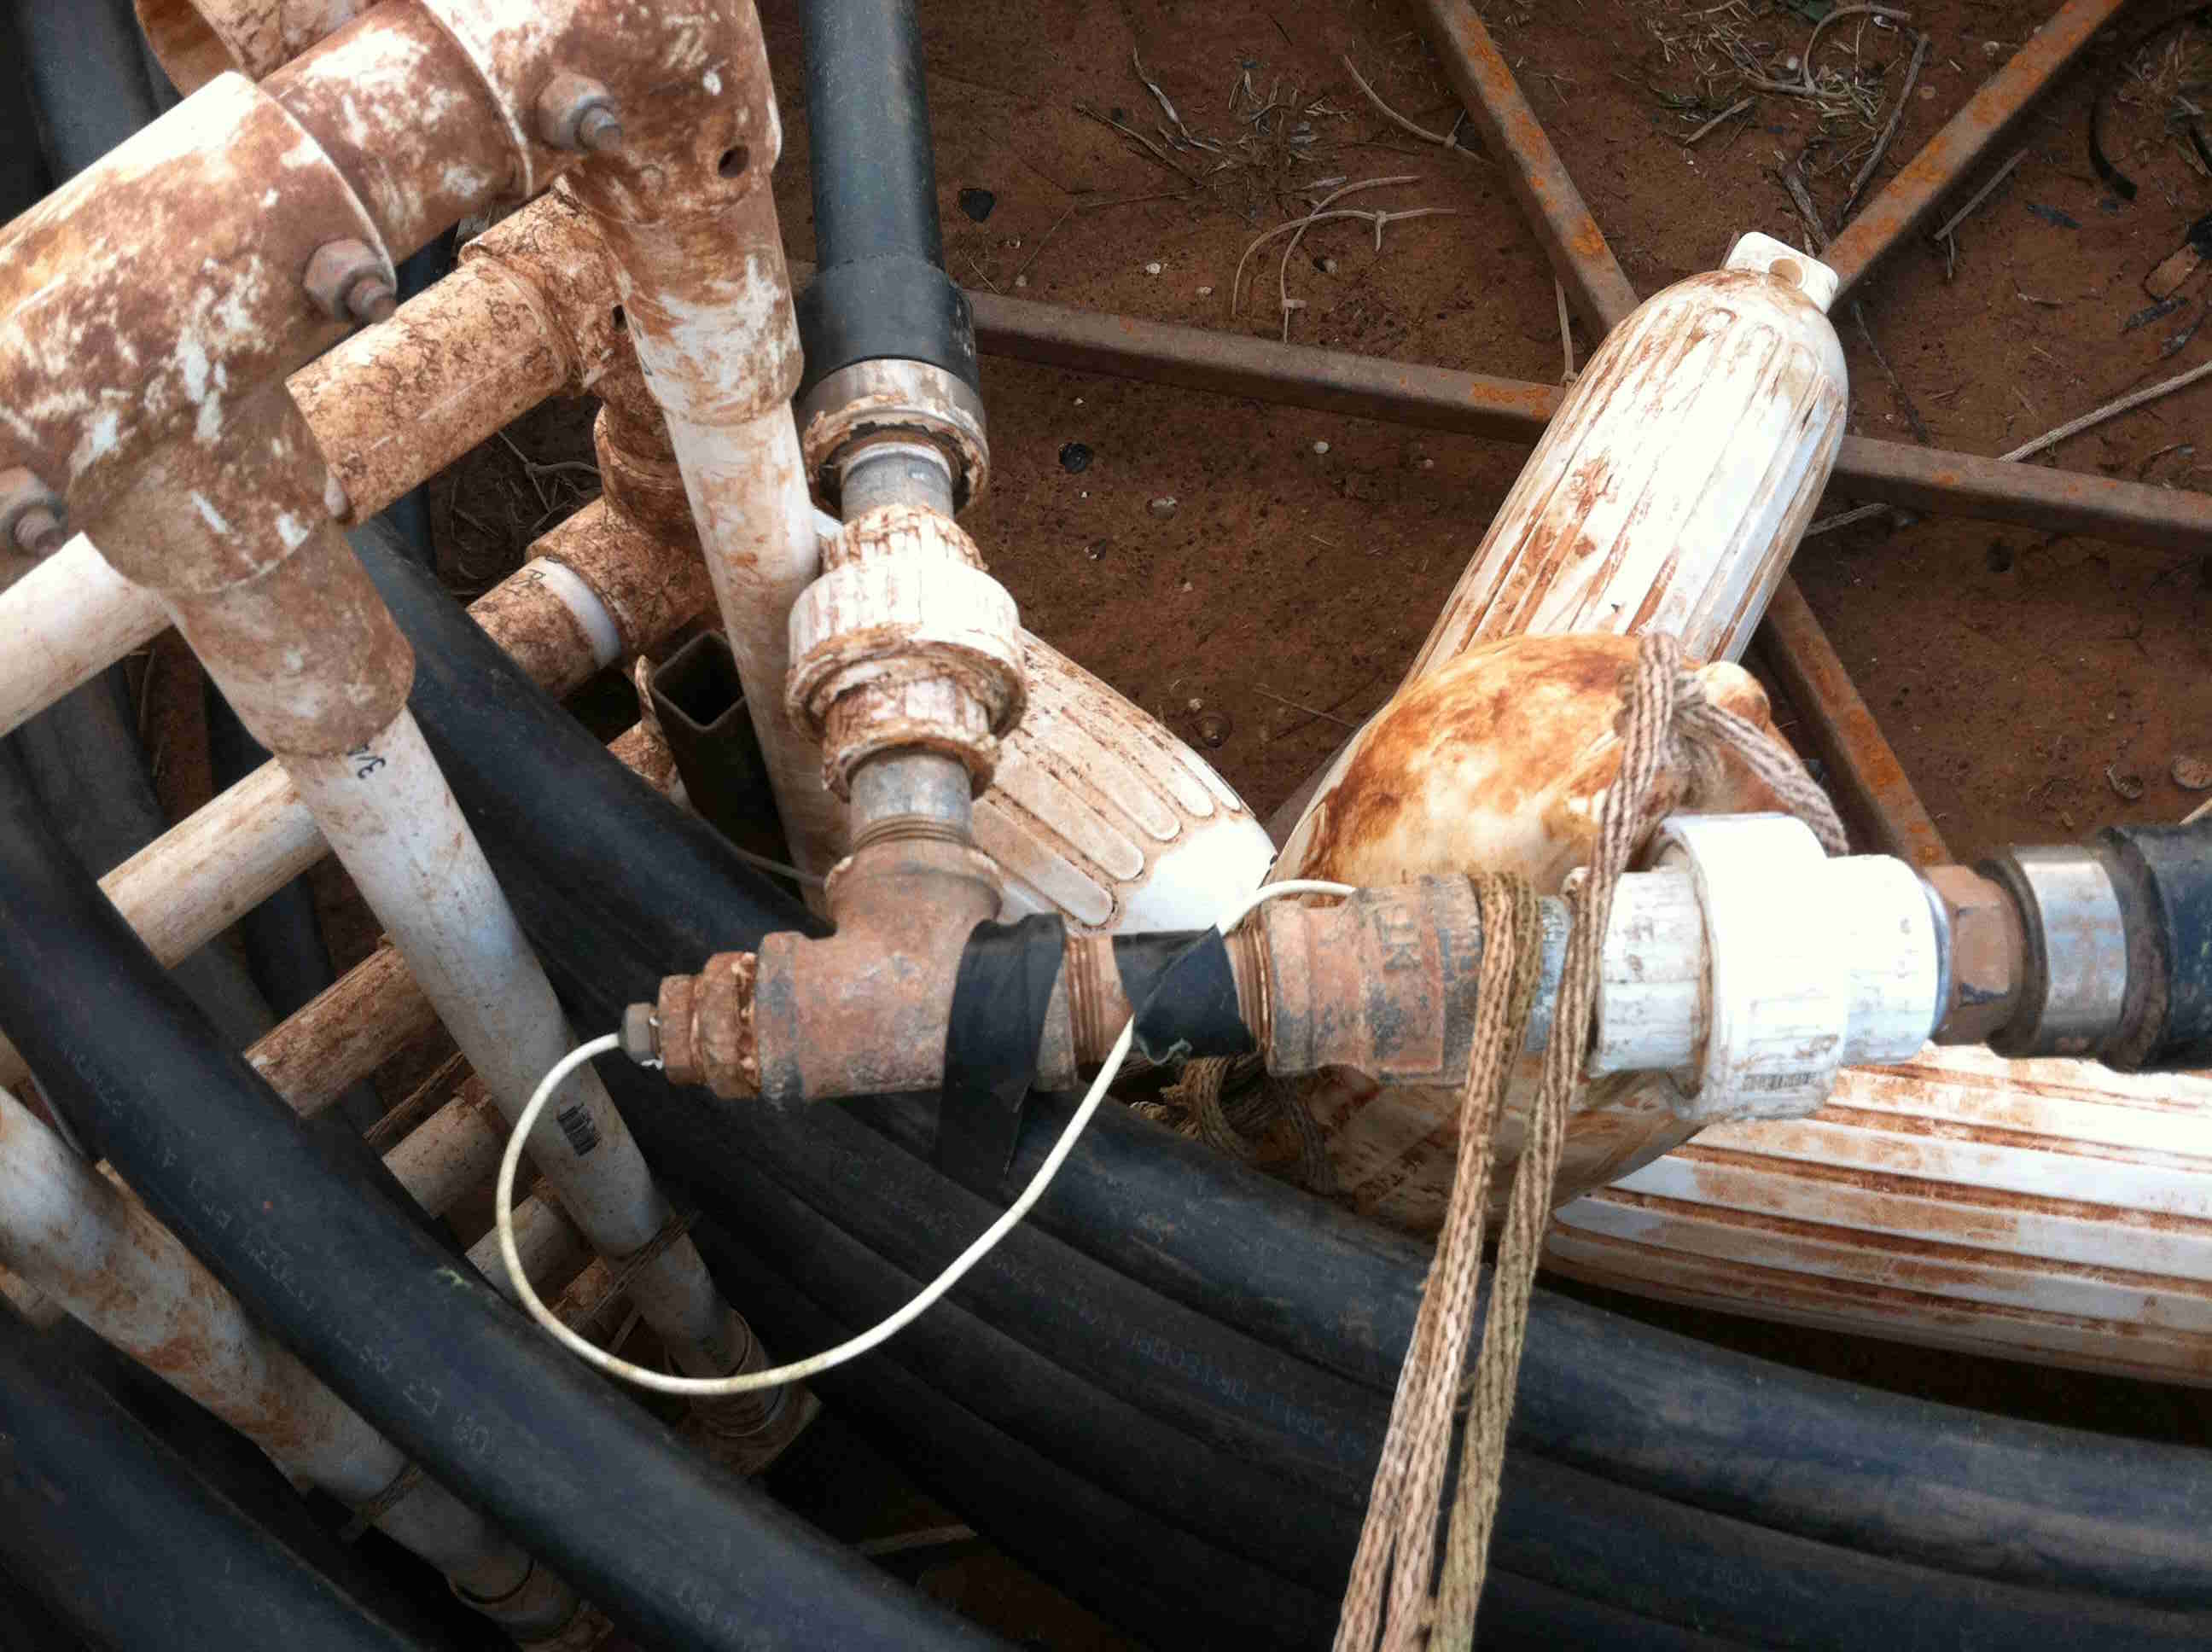
\includegraphics[width=0.8\textwidth]{In_Pipe_Thermistor.jpg}
		\caption[In-pipe thermistor used at SWHE inlet and oulet]{In-pipe thermistor used to measure the entering or exiting fluid temperature}
		\label{fig:ExpMethod:HeatRej:Apparatus:InPipeThermistor}
	\end{figure}


	\begin{figure}
		\centering
		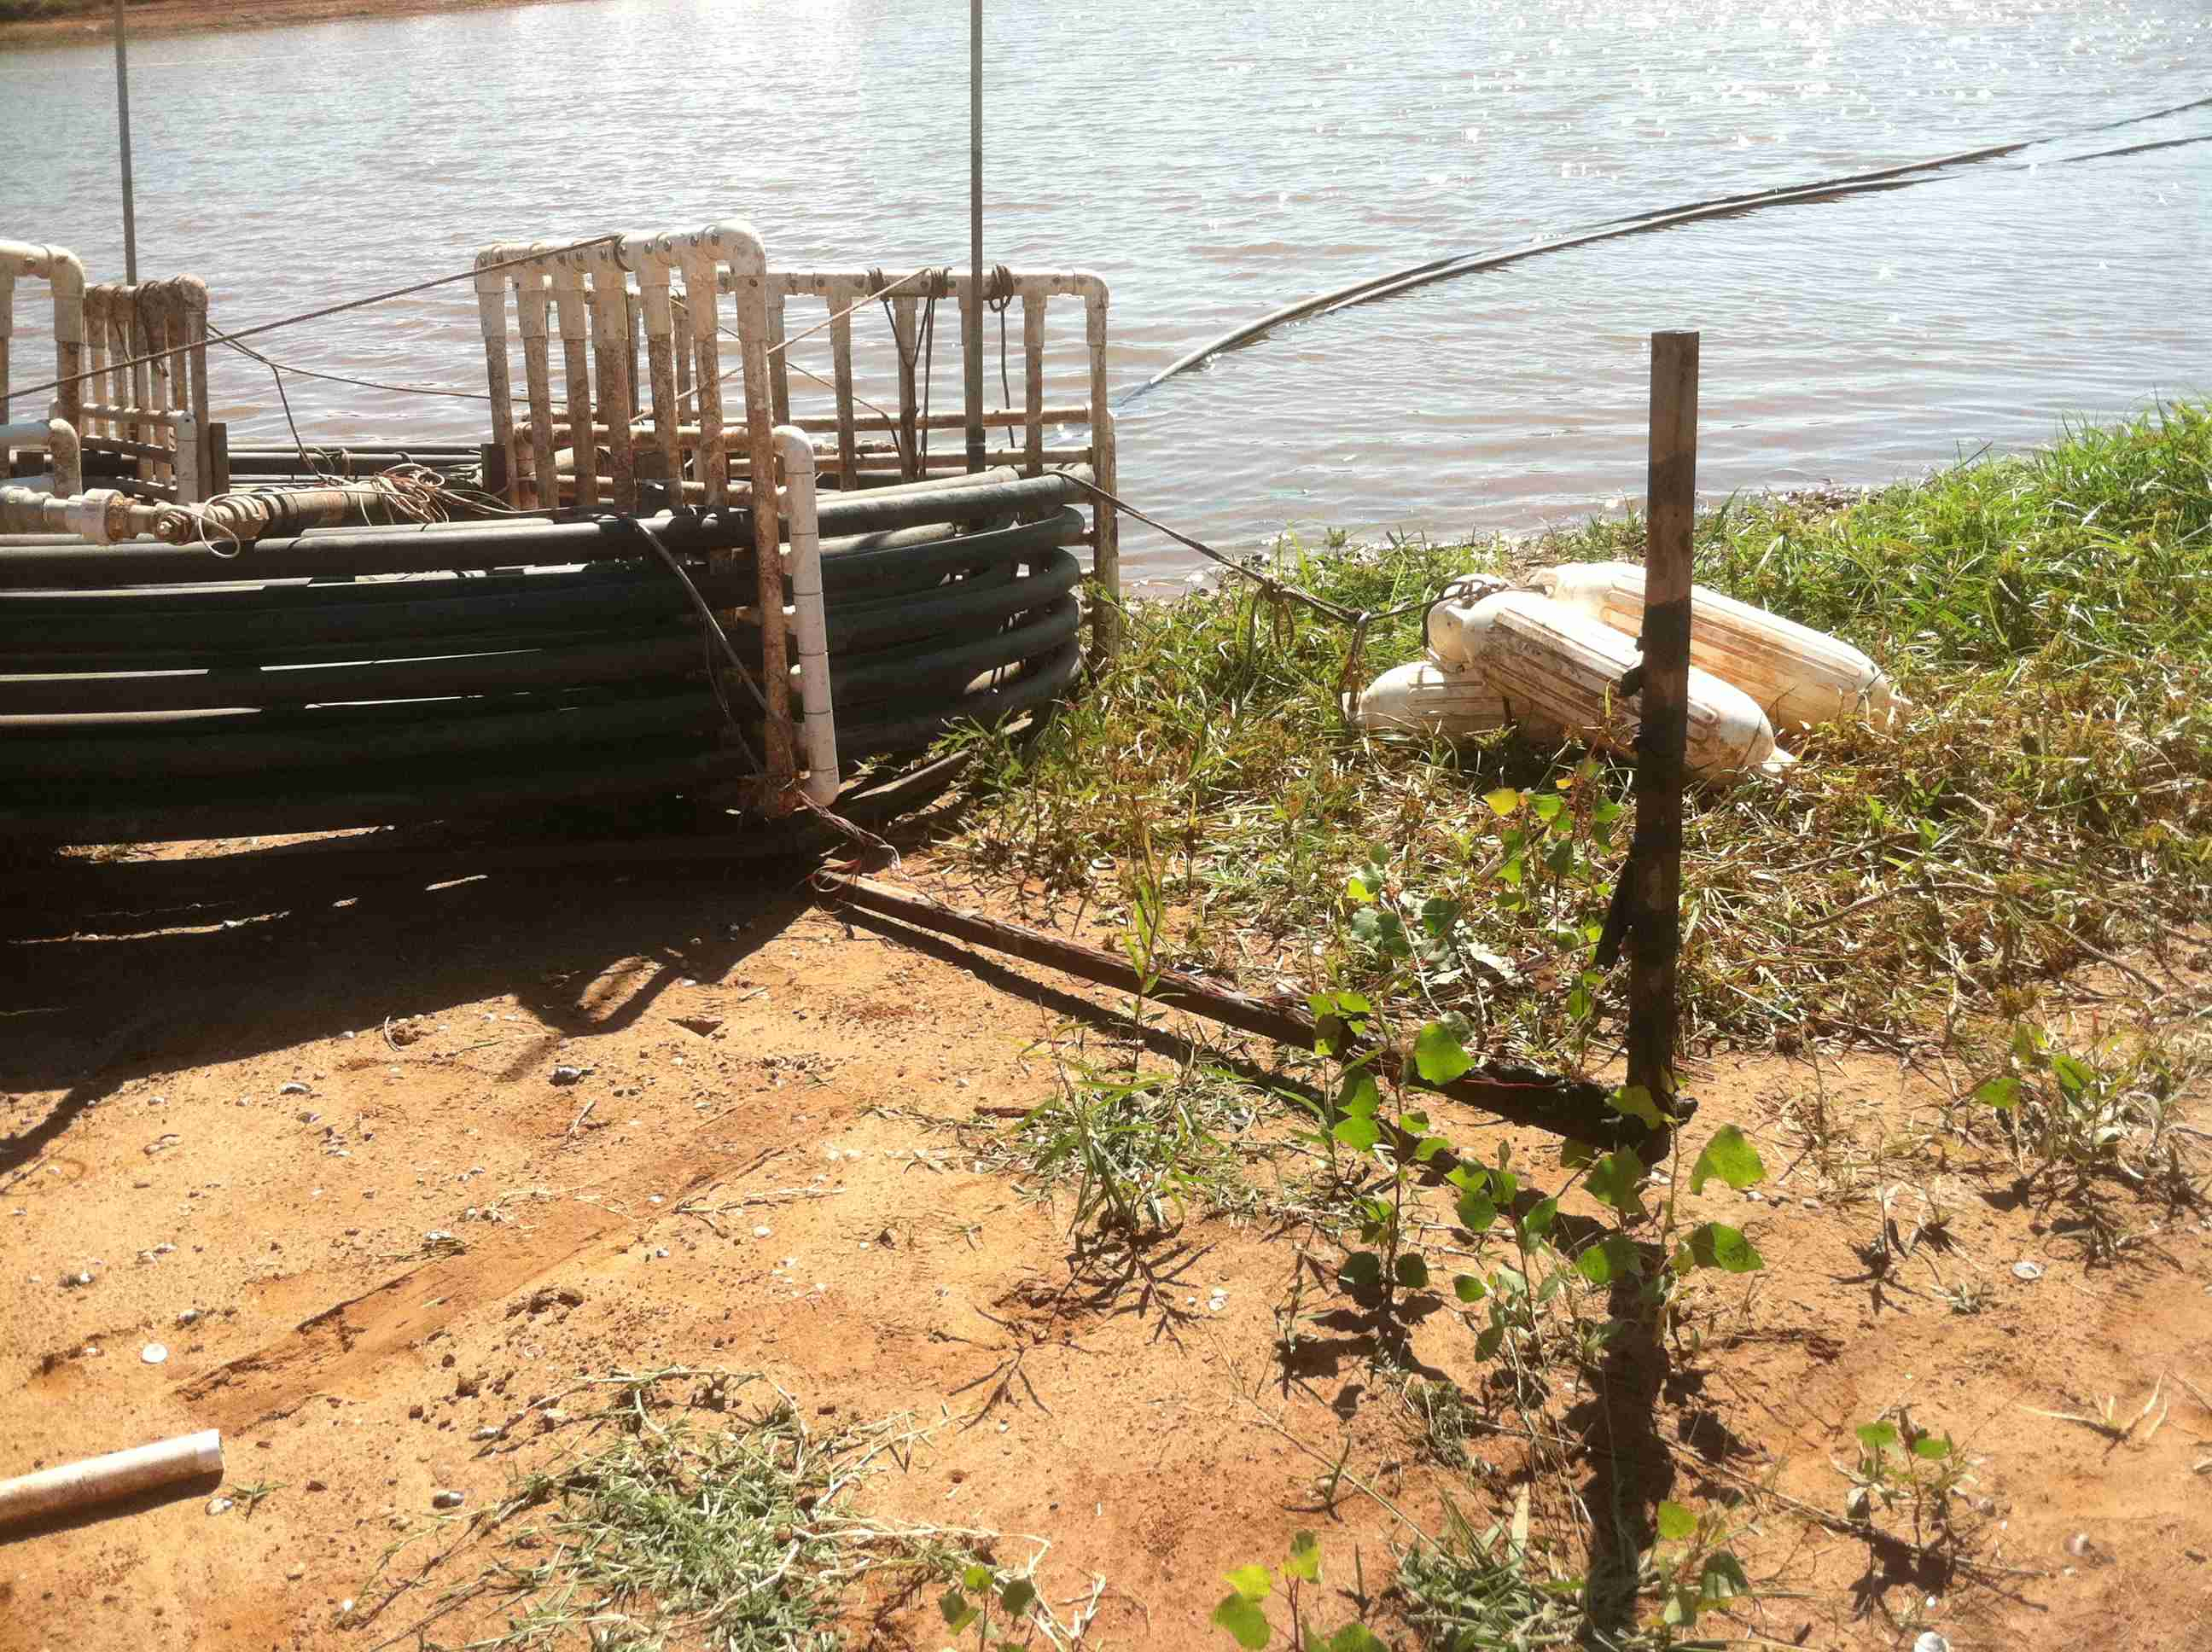
\includegraphics[width=0.8\textwidth]{L_Arm.jpg}
		\caption[L-arm on SWHE test frame]{L-arm at a distance of 4 ft.\ (1.2 m) away from coil used for measuring local pond temperature}
		\label{fig:ExpMethod:HeatRej:Apparatus:LArm}
	\end{figure}

Additionally, 14 other thermistors were also placed in the pond on two vertical pipes at a distance of approximately 30 ft.\ (9.1 m) and 100 ft.\ (30.5 m) away from the SWHE. Beginning at the pond bottom, the thermistors were spaced 18 in.\ (46 cm) apart vertically allowing for the measurement of the pond temperature profile at two separate locations. Actual thermistor water depth was determined by measuring the pond water level from a reference datum and applying a calibration determine the thermistor depth relative to the water surface. The flow meter and thermistors were all connected to a data logger recording data at 10 second intervals.

	\subsection{Methodology}
	\label{subsec:ExpMethod:HeatRej:Method}

To conduct each heat rejection experiment, a series of three tests were run on each coil configuration. Each test was composed of a series of eight incrementally increasing heat input set points up to 3.5 tons (12.5 kW). Once each heat rate was set, the experiment was allowed to run until steady state operating conditions were achieved, which was determined by examining the SWHE entering and exiting fluid temperature. Once steady state conditions were achieved, the experiment was allowed to run for another five minutes to collect data. The average of the data taken during the five minutes of steady state operation was then taken as the steady state operation point. The set point was then changed and the process repeated until the maximum heat rejection rate of 3.5 tons (12.5 kW) was reached and data collected.

A total of 27 spiral helical SWHE configurations were tested at the test pond. The nominal tube size was varied from 3/4 in.\ (19 mm), 1 in.\ (25 mm), and 1-1/4 in.\ (32 mm) SDR-11 HDPE. The smallest horizontal and vertical center-center tube spacing was varied from 1.3 in.\ (33 mm), 1.6 in.\ (41 mm), and 1.9 in.\ (48 mm) for each respective tube size. The medium and large horizontal and vertical center-center tube spacing was set at 2.625 in.\ (67 mm) and 4.125 in.\ (105 mm), regardless of tube size. Tables \ref{tab:ExpMethod:HeatRej:Method:0.75inTestSummaryTable}, \ref{tab:ExpMethod:HeatRej:Method:1inTestSummaryTable}, and  \ref{tab:ExpMethod:HeatRej:Method:1.25inTestSummaryTable} show the dates when each test series for each coil configuration was completed. Tables \ref{tab:ExpMethod:HeatRej:Method:SWHEGeometry1}, \ref{tab:ExpMethod:HeatRej:Method:SWHEGeometry2}, and \ref{tab:ExpMethod:HeatRej:Method:SWHEGeometry3} show the geometrical measurements for each respective spiral-helical SWHE coil configuration.

The testing and work performed on the spiral-helical SWHE are a continuation of work initiated by \cite{Hansen2011}. The tests indicated in \textit{\textcolor{blue}{blue italics}} are tests that occurred after the publication of \cite{Hansen2011}.

	\begin{table}
		\centering
		\caption[3/4 in.\ (19 mm) SWHE test summary]{3/4 in.\ (19 mm) SDR-11 HDPE spiral-helical SWHE test summary}
		\label{tab:ExpMethod:HeatRej:Method:0.75inTestSummaryTable}
		\begin{tabular}{|c|c|c|c|}
			\hline
			& \multicolumn{3}{|c|}{Test Dates} \\
			\hline\hline
			Vert/Horiz & 1.3 in.\ & 2.625 in.\ & 4.125 in.\ \\
			Spacing & (33 mm) & (67 mm) & (105 mm) \\
			\hline
			1.3 in.\ & \multirow{2}{*}{4/19--4/20/11} & 3/28--3/29-11 & \multirow{2}{*}{3/8/11} \\
			(33 mm) & & 4/8--4/11/11 & \\
			\hline
			2.625 in.\ & \multirow{2}{*}{4/21/11} & 3/26--3/27/11 & \multirow{2}{*}{3/2--3/5/11} \\
			(67 mm) & & 4/13--4/14/11 & \\
			\hline
			4.125 in.\ & \multirow{2}{*}{4/22--4/25/11} & \multirow{2}{*}{3/30--4/1/11} & \multirow{2}{*}{3/17--3/18/11} \\
			(105 mm) & & & \\
			\hline
		\end{tabular}
	\end{table}

	\begin{table}
	\centering
		\caption[1 in.\ (25 mm) SWHE test summary]{1 in.\ (25 mm) SDR-11 HDPE spiral-helical SWHE test summary}
		\label{tab:ExpMethod:HeatRej:Method:1inTestSummaryTable}
		\begin{tabular}{|c|c|c|c|}
			\hline
			& \multicolumn{3}{|c|}{Test Dates}\\
			\hline\hline
			Vert/Horiz& 1.6 in.\ & 2.625 in.\ & 4.125 in.\ \\
			Spacing & (41 mm) & (67 mm) & (105 mm) \\
			\hline
			1.6 in.\ & \multirow{2}{*}{10/4--10/5/11} & \multirow{2}{*}{9/15/11} & \multirow{2}{*}{\textit{\textcolor{blue}{11/17--11/18/11}}} \\
			(41 mm) & & & \\
			\hline
			2.625 in.\ & \multirow{2}{*}{\textit{\textcolor{blue}{10/6--10/7/11}}} & \multirow{2}{*}{9/7--9/8/11} & \multirow{2}{*}{\textit{\textcolor{blue}{11/28--11/29/11}}} \\
			(67 mm) & & & \\
			\hline
			4.125 in.\ & \multirow{2}{*}{\textit{\textcolor{blue}{10/12--10/13/11}}} & \multirow{2}{*}{9/13/11} & \multirow{2}{*}{6/17--6/20/11} \\
			(105 mm) & & & \\
			\hline
		\end{tabular}
	\end{table}

	\begin{table}
	\centering
		\caption[1-1/4 in.\ (32 mm) SWHE test summary]{1-1/4 in.\ (32 mm) SDR-11 HDPE spiral-helical SWHE test summary}
		\label{tab:ExpMethod:HeatRej:Method:1.25inTestSummaryTable}
		\begin{tabular}{|c|c|c|c|}
			\hline
			& \multicolumn{3}{|c|}{Test Dates}\\
			\hline\hline
			Vert/Horiz & 1.9 in.\ & 2.625 in.\ & 4.125 in.\ \\
			Spacing & (48 mm) & (67 mm) & (105 mm) \\
			\hline
			1.9 in.\ & \multirow{2}{*}{\textit{\textcolor{blue}{10/20--10/24/11}}} & \multirow{2}{*}{6/20--6/22/11} & \multirow{2}{*}{9/20--9/21/11} \\
			(48 mm) & & & \\
			\hline
			2.625 in.\ & \multirow{2}{*}{\textit{\textcolor{blue}{10/26--10/31/11}}} & \multirow{2}{*}{6/15--6/16/11} & \multirow{2}{*}{9/22/11} \\
			(67 mm) & & & \\
			\hline
			4.125 in.\ & \multirow{2}{*}{\textit{\textcolor{blue}{11/14--11/15/11}}} & \multirow{2}{*}{\textit{\textcolor{blue}{12/1--12/2/11}}} & \multirow{2}{*}{9/26/11} \\
			(105 mm) & & & \\
			\hline
		\end{tabular}
	\end{table}

	\begin{table}
	\centering
		\caption[3/4 in.\ (19 mm) spiral-helical SWHE geometry]{Geometry of 3/4 in.\ (19 mm) spiral-helical surface water heat exchangers}
		\label{tab:ExpMethod:HeatRej:Method:SWHEGeometry1}
		\begin{tabular}{|c|c|c|c|}
		\hline
		& \multicolumn{3}{|c|}{Coil Heights}\\
		\hline\hline
		Vert/Horiz & \multirow{2}{*}{1.3 in.\ (33 mm)} & \multirow{2}{*}{2.626 in.\ (67 mm)} & \multirow{2}{*}{4.125 in.\ (105 mm)} \\
		Spacing &  &  &  \\
		\hline
		1.3 in.\ (33 mm) & 8.5 in.\ (21.6 cm) & 7 in.\ (17.8 cm) & 7 in.\ (17.8 cm) \\
		\hline
		2.625 in.\ (67 mm) & 14.2 in.\ (36 cm) & 14.2 in.\ (36 cm) & 11.6 in.\ (29.5 cm) \\
		\hline
		4.125 in.\ (105 mm) & 21.7 in.\ (55.1 cm) & 21.7 in.\ (55.1 cm) & 17.5 in.\ (44.5 cm) \\
		\hline\hline
		Coil OD & \multicolumn{3}{|c|}{5.5 ft.\ (1.7 m)} \\
		\hline
		Coil ID & \multicolumn{3}{|c|}{4 ft.\ (1.2 m)}\\
		\hline
		\end{tabular}
	\end{table}

	\begin{table}
	\centering
		\caption[1 in.\ (25 mm) spiral-helical SWHE geometry]{Geometry of 1 in.\ (25 mm) spiral-helical surface water heat exchangers}
		\label{tab:ExpMethod:HeatRej:Method:SWHEGeometry2}
		\begin{tabular}{|c|c|c|c|}
		\hline
		& \multicolumn{3}{|c|}{Coil Heights}\\
		\hline\hline
		Vert/Horiz & \multirow{2}{*}{1.6 in.\ (41 mm)} & \multirow{2}{*}{2.626 in.\ (67 mm)} & \multirow{2}{*}{4.125 in.\ (105 mm)} \\
		Spacing &  &  &  \\
		\hline
		1.6 in.\ (41 mm) & 10 in.\ (25.4 cm) & 8 in.\ (20.3 cm) & 11 in.\ (28 cm) \\
		\hline
		2.625 in.\ (67 mm) & 15 in.\ (38.1 cm) & 12 in.\ (30.5 cm) & 14 in.\ (35.6 cm) \\
		\hline
		4.125 in.\ (105 mm) & 22 in.\ (55.6 cm) & 17 in.\ (43.2 cm) & 17 in.\ (43.2 cm) \\
		\hline\hline
		Coil OD & \multicolumn{3}{|c|}{6.5 ft.\ (2 m)} \\
		\hline
		Coil ID & \multicolumn{3}{|c|}{4 ft.\ (1.2 m)}\\
		\hline
		\end{tabular}
	\end{table}

	\begin{table}
	\centering
		\caption[1-1/4 in.\ (32 mm) spiral-helical SWHE geometry]{Geometry of 1-1/4 in.\ (32 mm) spiral-helical surface water heat exchangers}
		\label{tab:ExpMethod:HeatRej:Method:SWHEGeometry3}
		\begin{tabular}{|c|c|c|c|}
		\hline
		& \multicolumn{3}{|c|}{Coil Heights}\\
		\hline\hline
		Vert/Horiz & \multirow{2}{*}{1.9 in.\ (48 mm)} & \multirow{2}{*}{2.626 in.\ (67 mm)} & \multirow{2}{*}{4.125 in.\ (105 mm)} \\
		Spacing &  &  &  \\
		\hline
		1.9 in.\ (48 mm) & 11 in.\ (28.9 cm) & 10 in.\ (25.4 cm) & 10 in.\ (25.4 cm) \\
		\hline
		2.625 in.\ (67 mm) & 17 in.\ (43.2 cm) & 14 in.\ (35.6 cm) & 14 in.\ (35.6 cm) \\
		\hline
		4.125 in.\ (105 mm) & 22 in.\ (55.9 cm) & 18 in.\ (45.7 cm) & 18 in.\ (45.7 cm) \\
		\hline\hline
		Coil OD & \multicolumn{3}{|c|}{8 ft.\ (2.4 m)}\\
		\hline
		Coil ID & \multicolumn{3}{|c|}{4 ft.\ (1.2 m)}\\
		\hline
		\end{tabular}
	\end{table}

\section{Heat Extraction Experiments}
\label{sec:ExpMethod:HeatExtr}

	\subsection{Facility}
	\label{subsec:ExpMethod:HeatExtr:Facility}

Heat extraction tests performed on the spiral-helical SWHE were conducted at two separate locations. Testing began at the test pond which can be seen in Figure \ref{fig:ExpMethod:HeatRej:Facility:PondMain}. However, because 2011 was one of the warmest years on record, the tests were moved indoors to a research facility with a more controlled environment. An exterior and interior view of the lab facility can be seen in Figures \ref{fig:ExpMethod:HeatExtr:Facility:ExtrExpERLOutside} and \ref{fig:ExpMethod:HeatExtr:Facility:ExtrExpERLInside}, respectively. By extracting heat from the SWHE, we were expecting the SWHE surface temperature to drop below the freezing point of the pond water, thereby causing coil icing conditions. In order to create these conditions without sufficiently cold weather, the experiment was moved to a location where the ambient temperature could be more readily controlled.

	\begin{figure}
		\centering
		\subfloat[Outside view of laboratory facility where indoor experiments were performed]{
			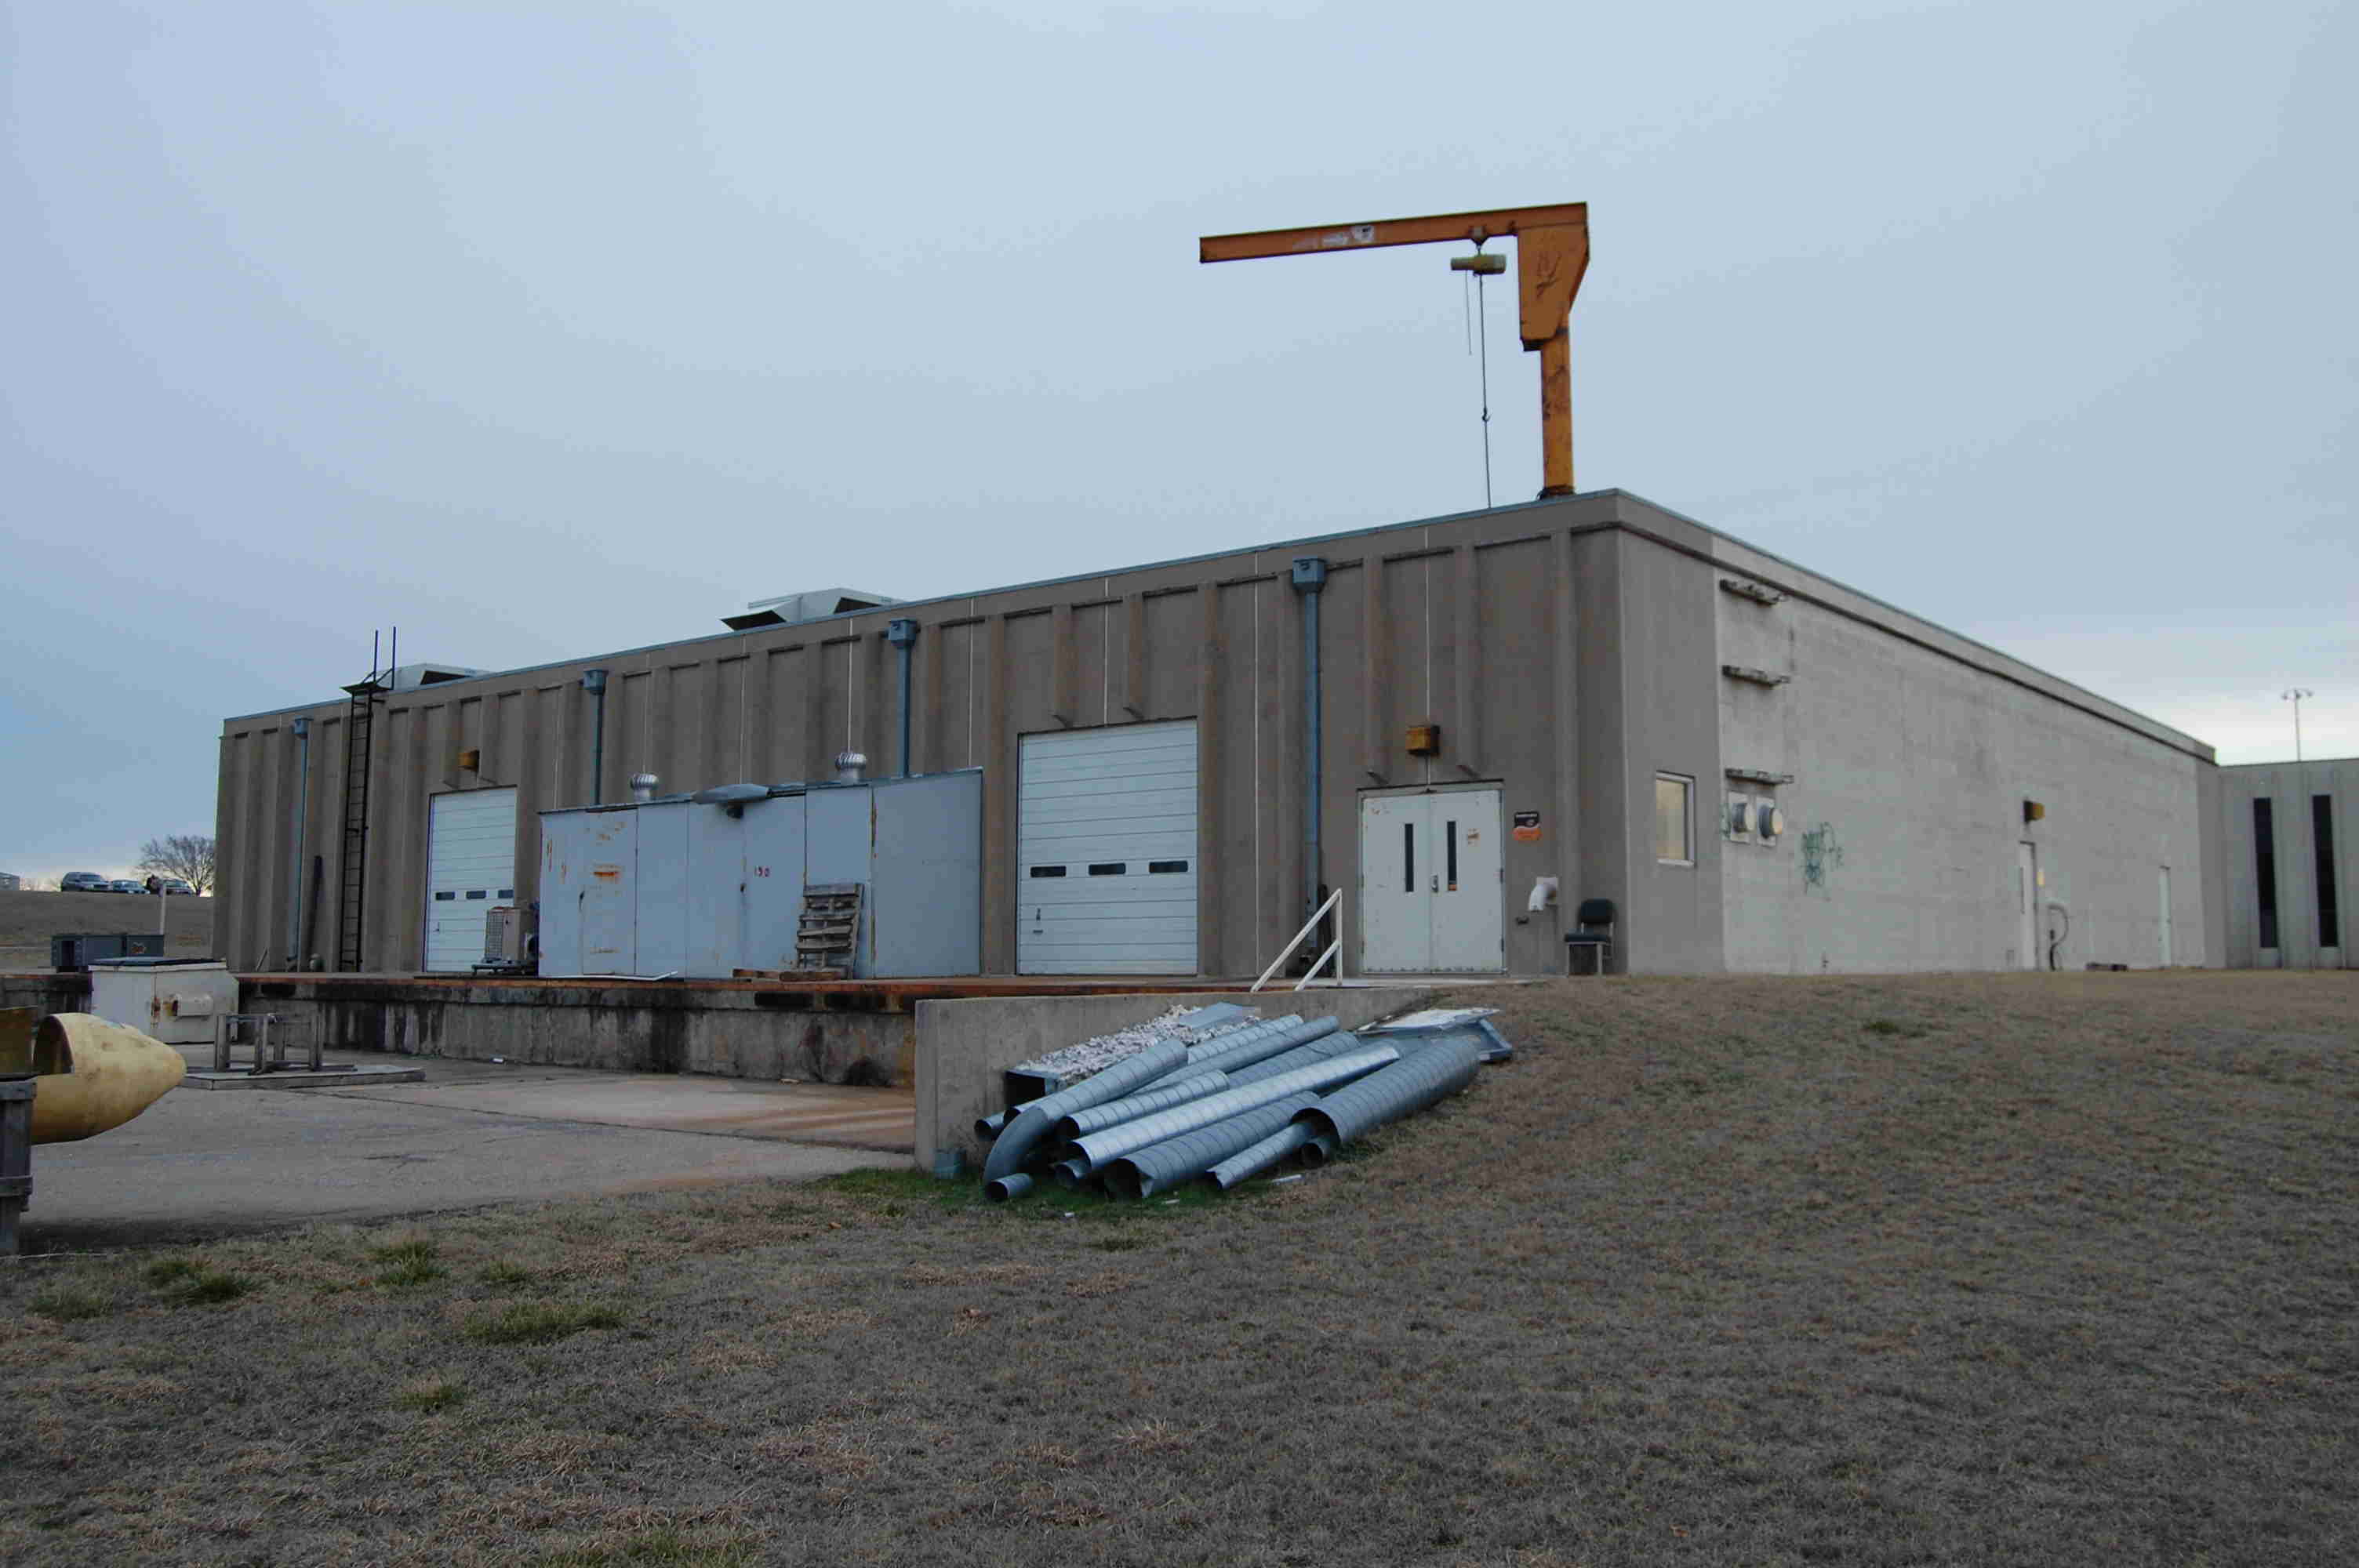
\includegraphics[width=0.47\textwidth]{ERL_Outside.jpg}
			\label{fig:ExpMethod:HeatExtr:Facility:ExtrExpERLOutside}}
		\,
		\subfloat[Inside view of laboratory facility where indoor experiments were performed]{
			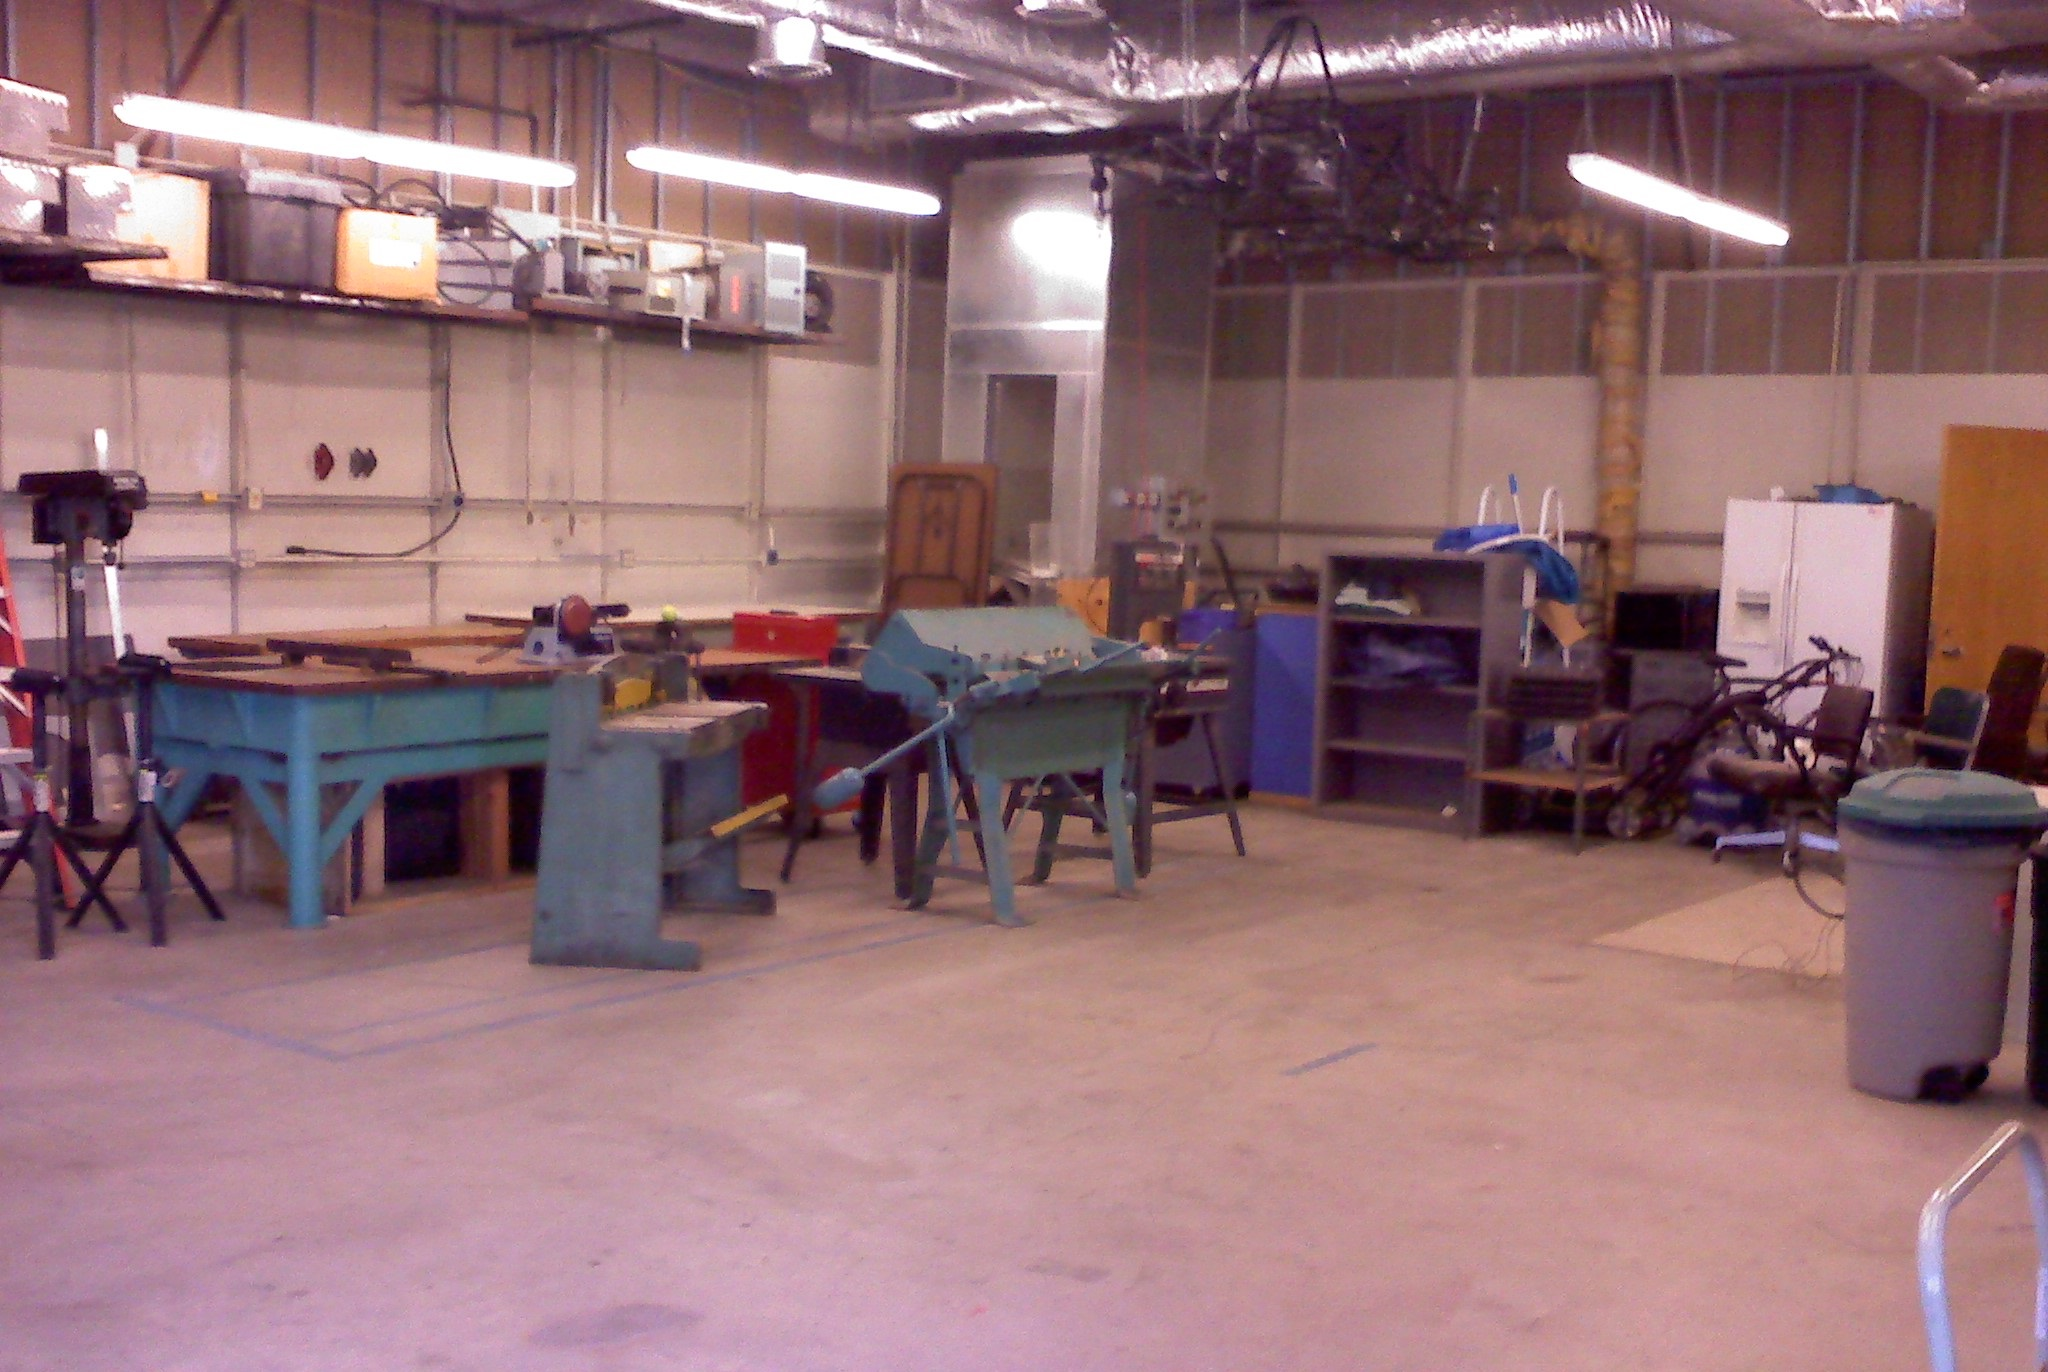
\includegraphics[width=0.47\textwidth]{ERL_Inside.jpg}
			\label{fig:ExpMethod:HeatExtr:Facility:ExtrExpERLInside}}
		\caption[Indoor test facility]{Test facility where indoor testing took place}
		\label{fig:ExpMethod:HeatRej:Facility:ERL}
	\end{figure}


	\subsection{Apparatus}
	\label{subsec:ExpMethod:HeatExtr:Apparatus}

To conduct experiments on spiral-helical SWHE under heat extraction conditions, a new trailer was purchased and the heat extraction experiment was constructed inside. This new trailer can be seen in Figure \ref{fig:ExpMethod:HeatExtr:Apparatus:ExtrExpTrailerOutsidePhoto}.

The heat extraction experiment consisted of two reversible heat pumps connected in parallel with a total nominal capacity of 4 tons (14.1 kW). One heat pump was a water-water heat pump with a nominal capacity of 3 tons (10.6 kW) while the remaining heat pump was a water-air heat pump with a nominal capacity of 1 ton (3.5 kW). Also part of the heat extraction experiment were circulation pumps, calibrated turbine flow meters, and multiple valves. In-pipe thermistors, as seen in Figure \ref{fig:ExpMethod:HeatRej:Apparatus:InPipeThermistor}  were placed at the inlet and outlet of the condenser and evaporator sides of the heat pumps, as well as at the SWHE inlet and outlet. Data loggers were placed inside of the trailer to record the data. A photo of the inside of the heat pump trailer can be seen in Figure \ref{fig:ExpMethod:HeatExtr:Apparatus:ExtrExpTrailerInsidePhoto}. A schematic of the heat extraction equipment located inside of the trailer can be seen in Figure \ref{fig:ExpMethod:HeatExtr:Apparatus:ExtrExpTrailerSchematic}.

	\begin{figure}
		\centering
		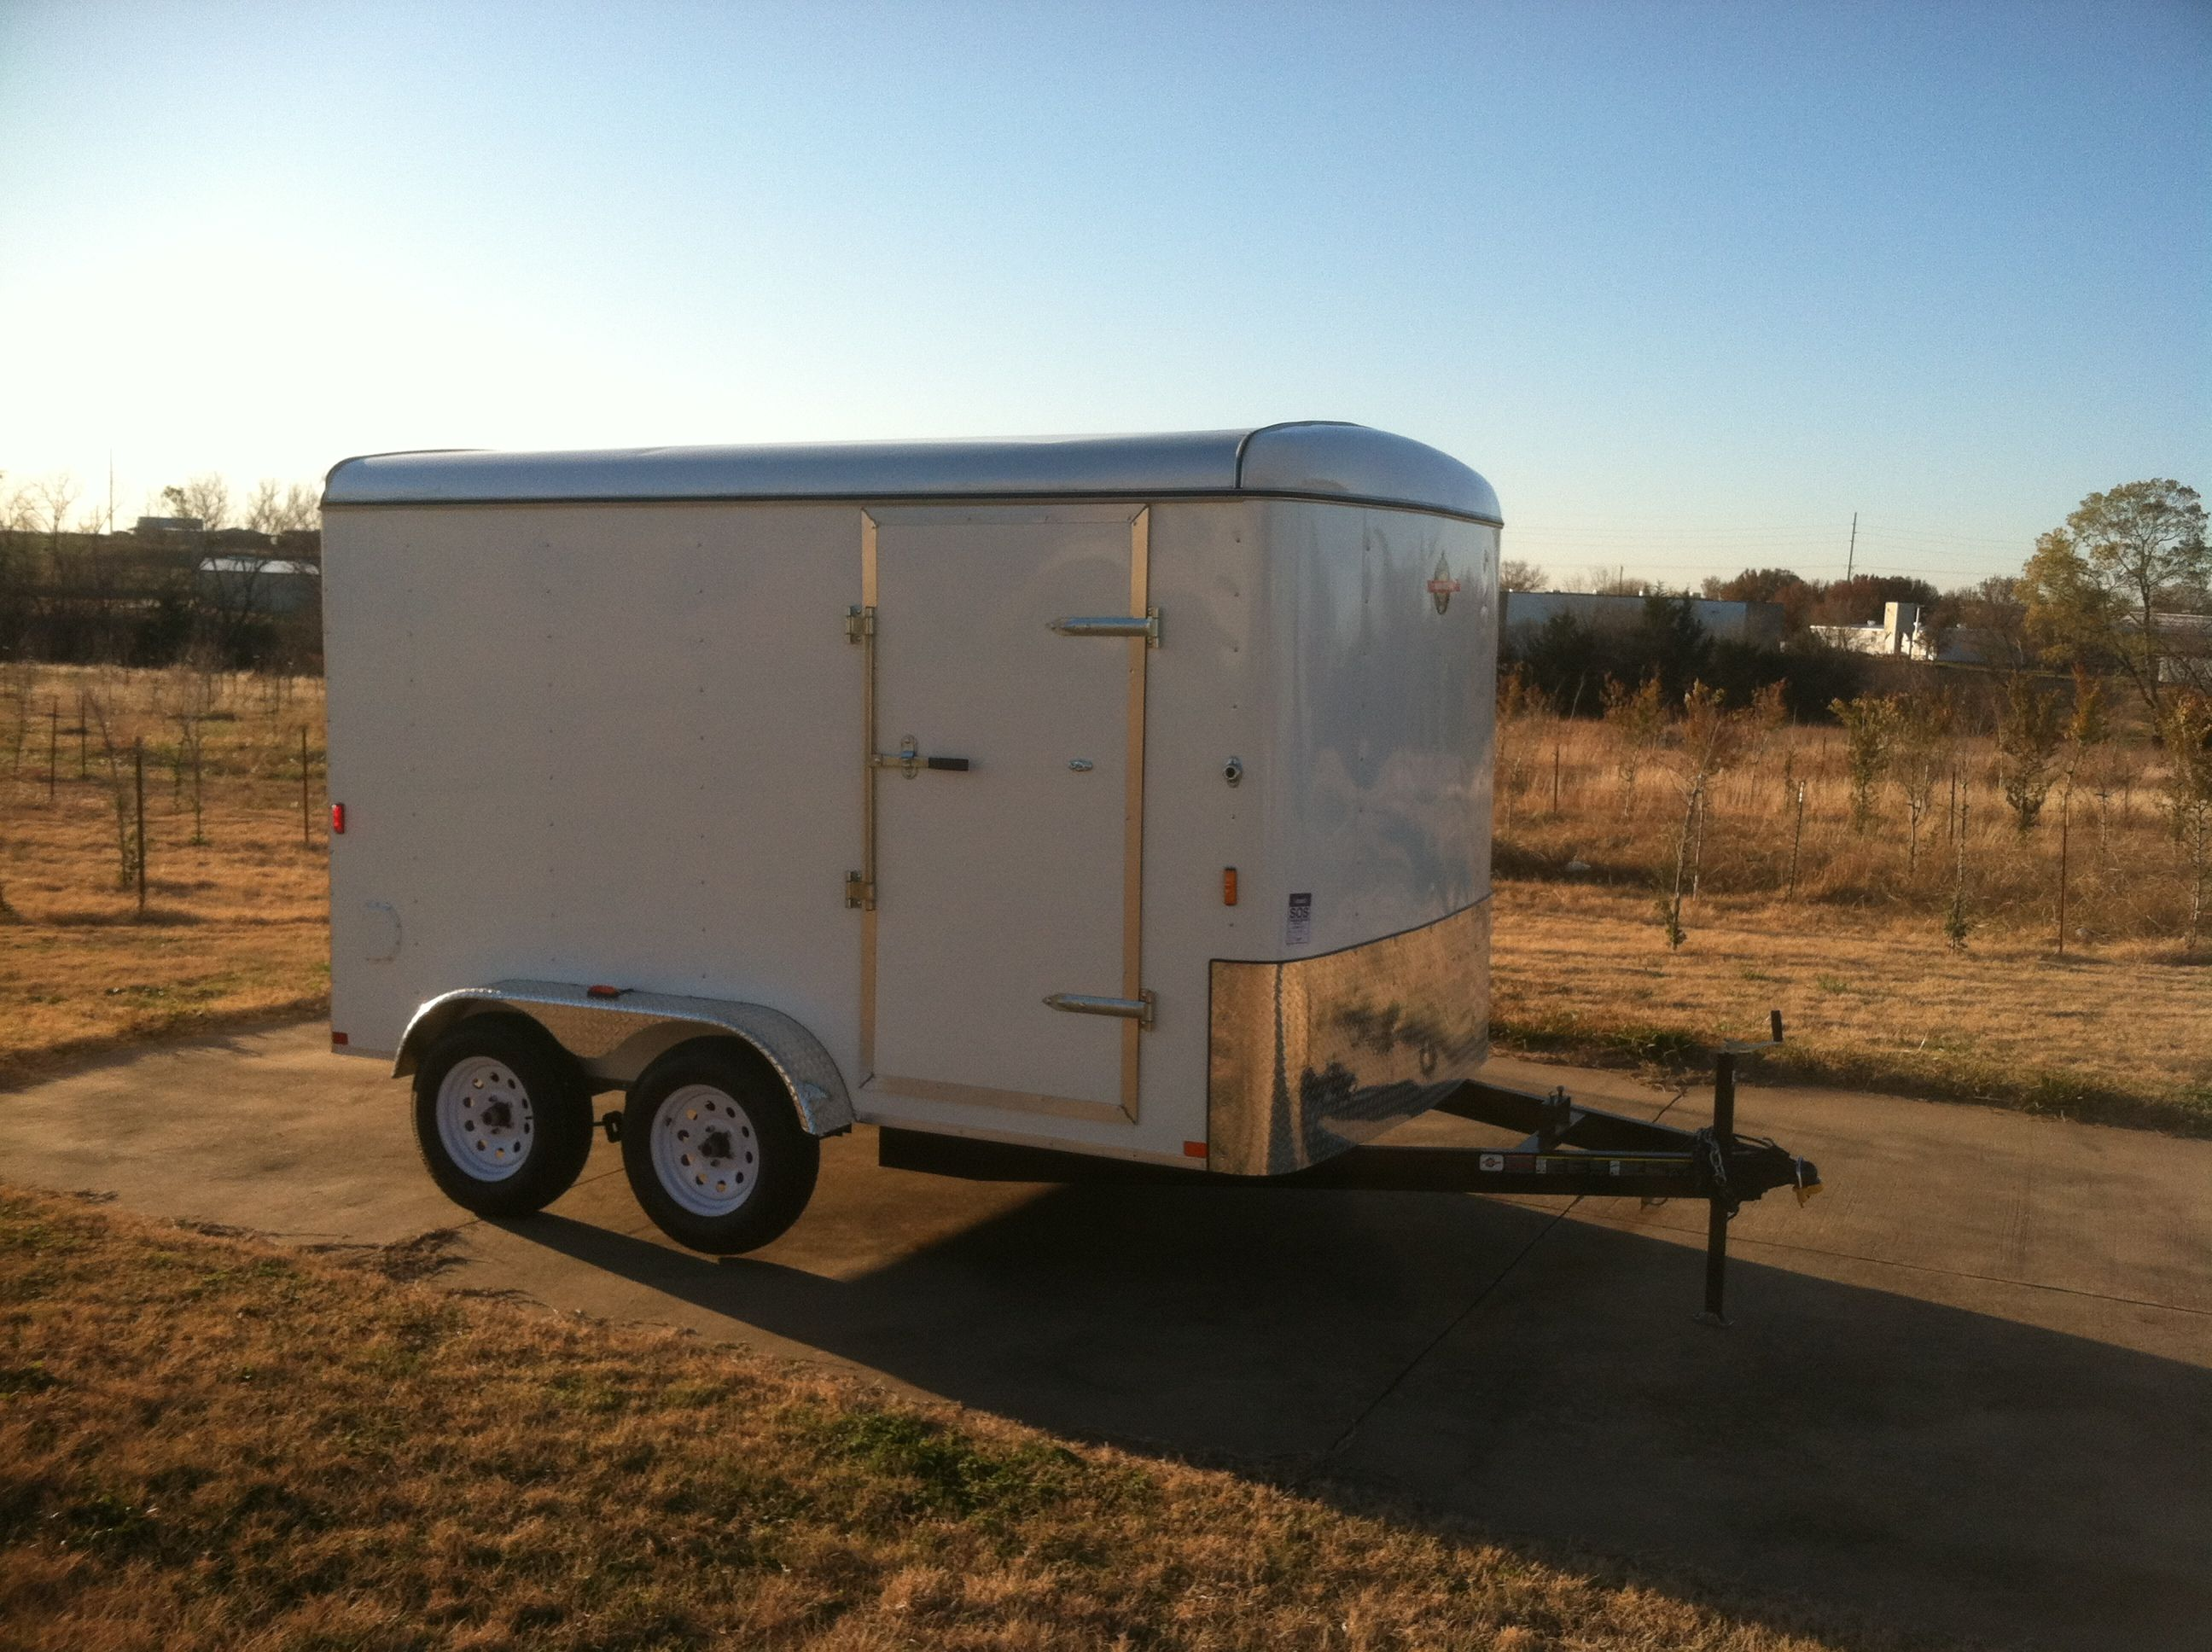
\includegraphics[width=0.8\textwidth]{Outside_Trailer.jpg}
		\caption[Heat extraction experiment trailer]{Trailer purchased for heat extraction experiment}
		\label{fig:ExpMethod:HeatExtr:Apparatus:ExtrExpTrailerOutsidePhoto}
	\end{figure}

	\begin{figure}
		\centering
		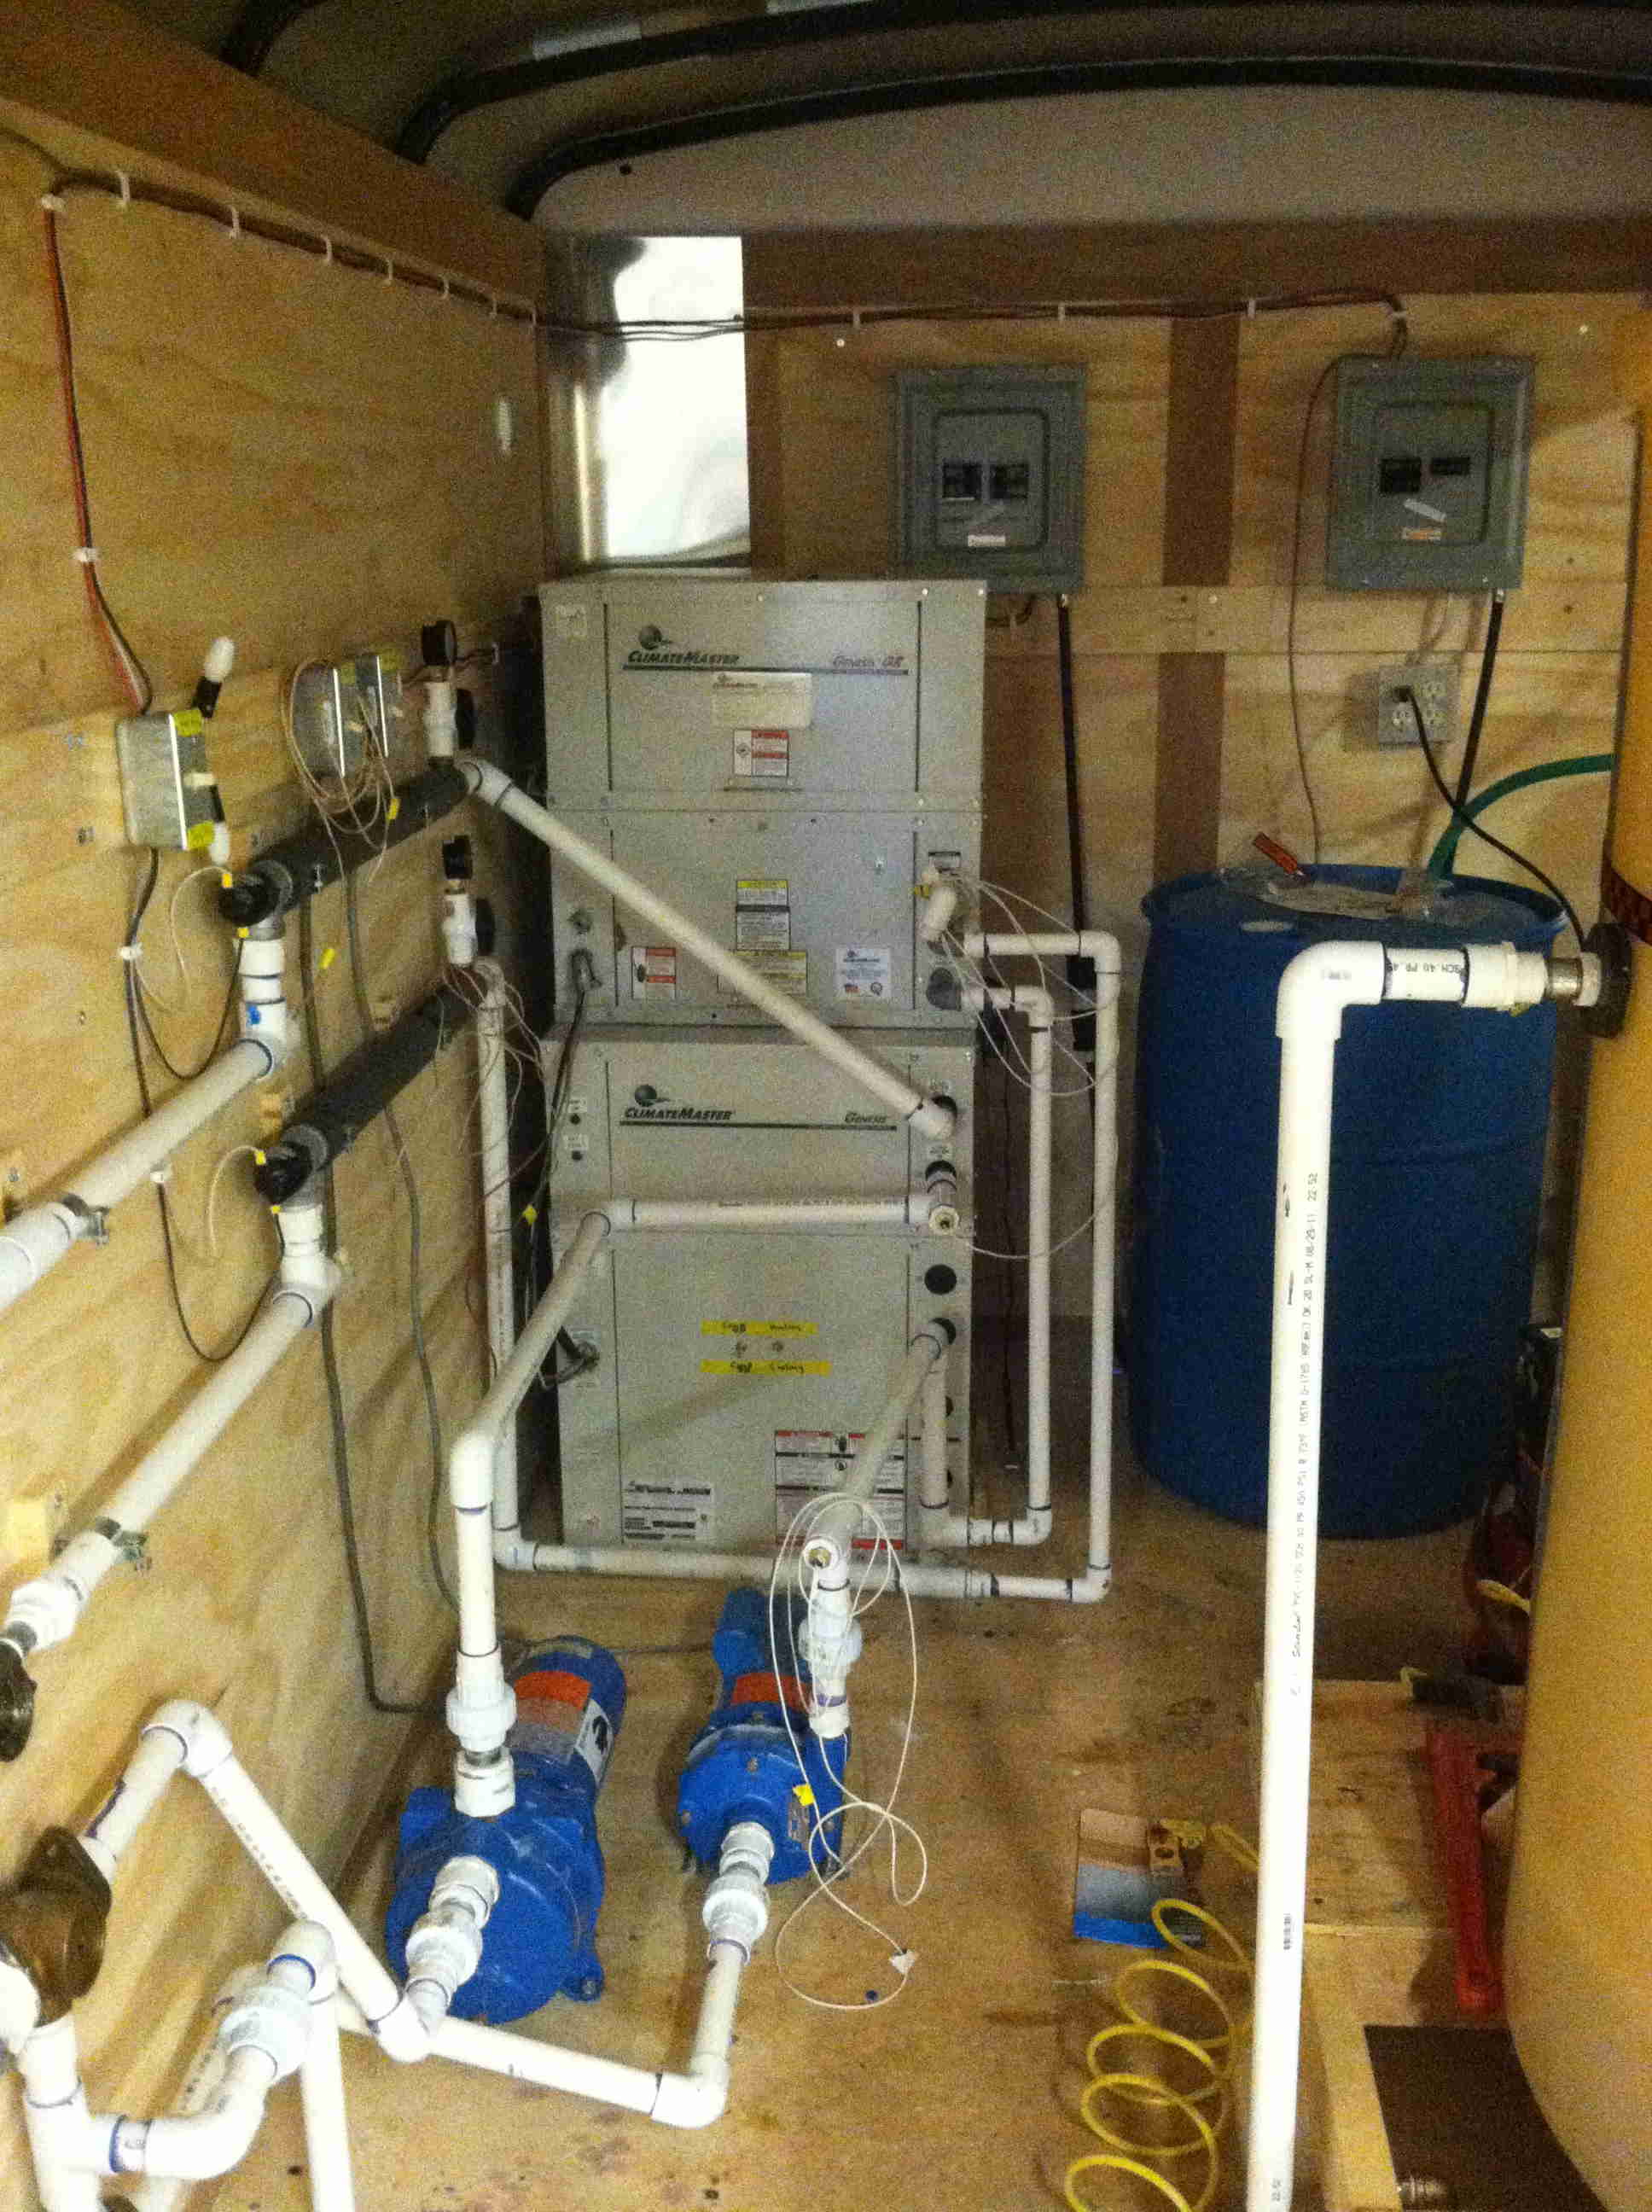
\includegraphics[width=0.8\textwidth]{Inside_Trailer.jpg}
		\caption[Inside view of heat extraction trailer]{Heat extraction experiment constructed inside new trailer}
		\label{fig:ExpMethod:HeatExtr:Apparatus:ExtrExpTrailerInsidePhoto}
	\end{figure}

	\begin{figure}
		\centering
		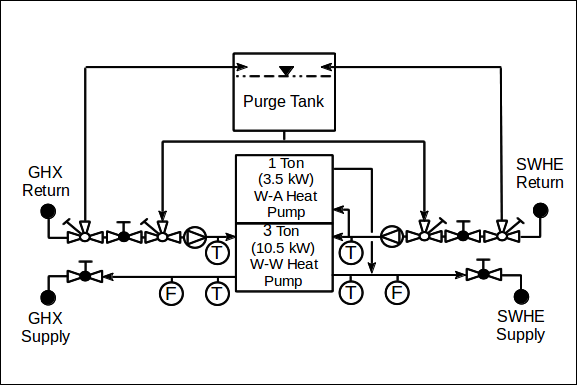
\includegraphics[width=0.8\textwidth]{Exp_Setup_Extraction.png}
		\caption[Schematic of heat extraction equipment in trailer]{Schematic of heat extraction equipment in trailer}
		\label{fig:ExpMethod:HeatExtr:Apparatus:ExtrExpTrailerSchematic}
	\end{figure}

As stated earlier, due to weather limitations, heat extraction tests were run at two separate locations, the test pond and the indoor laboratory facility. Because we were extracting heat from the SWHE, we expected ice to form on the coil. To quantify this ice formation, a new coil testing platform was constructed. The intent of this platform was to quantify the amount of ice formed on the SWHE by using load cells to directly measure the coil buoyancy and thus infer the amount of ice formed.

In order to counteract the upward buoyancy force of the ice, a weighted frame was constructed which would be sufficiently heavy so that it would counteract the buoyancy of the ice. This frame was also used to facilitate positioning of the coil in the water by allowing us to remove the coil from the pond with minimal effort. The weighted support frame's outside dimensions were 9.5 ft.\ x 9.5 ft.\ (2.9 x 2.9 m) and weighed approximately 400 lb (181 kg). The weighted support frame can be seen in Figure \ref{fig:ExpMethod:HeatExtr:Apparatus:WeightedFrame}.

	\begin{figure}
		\centering
		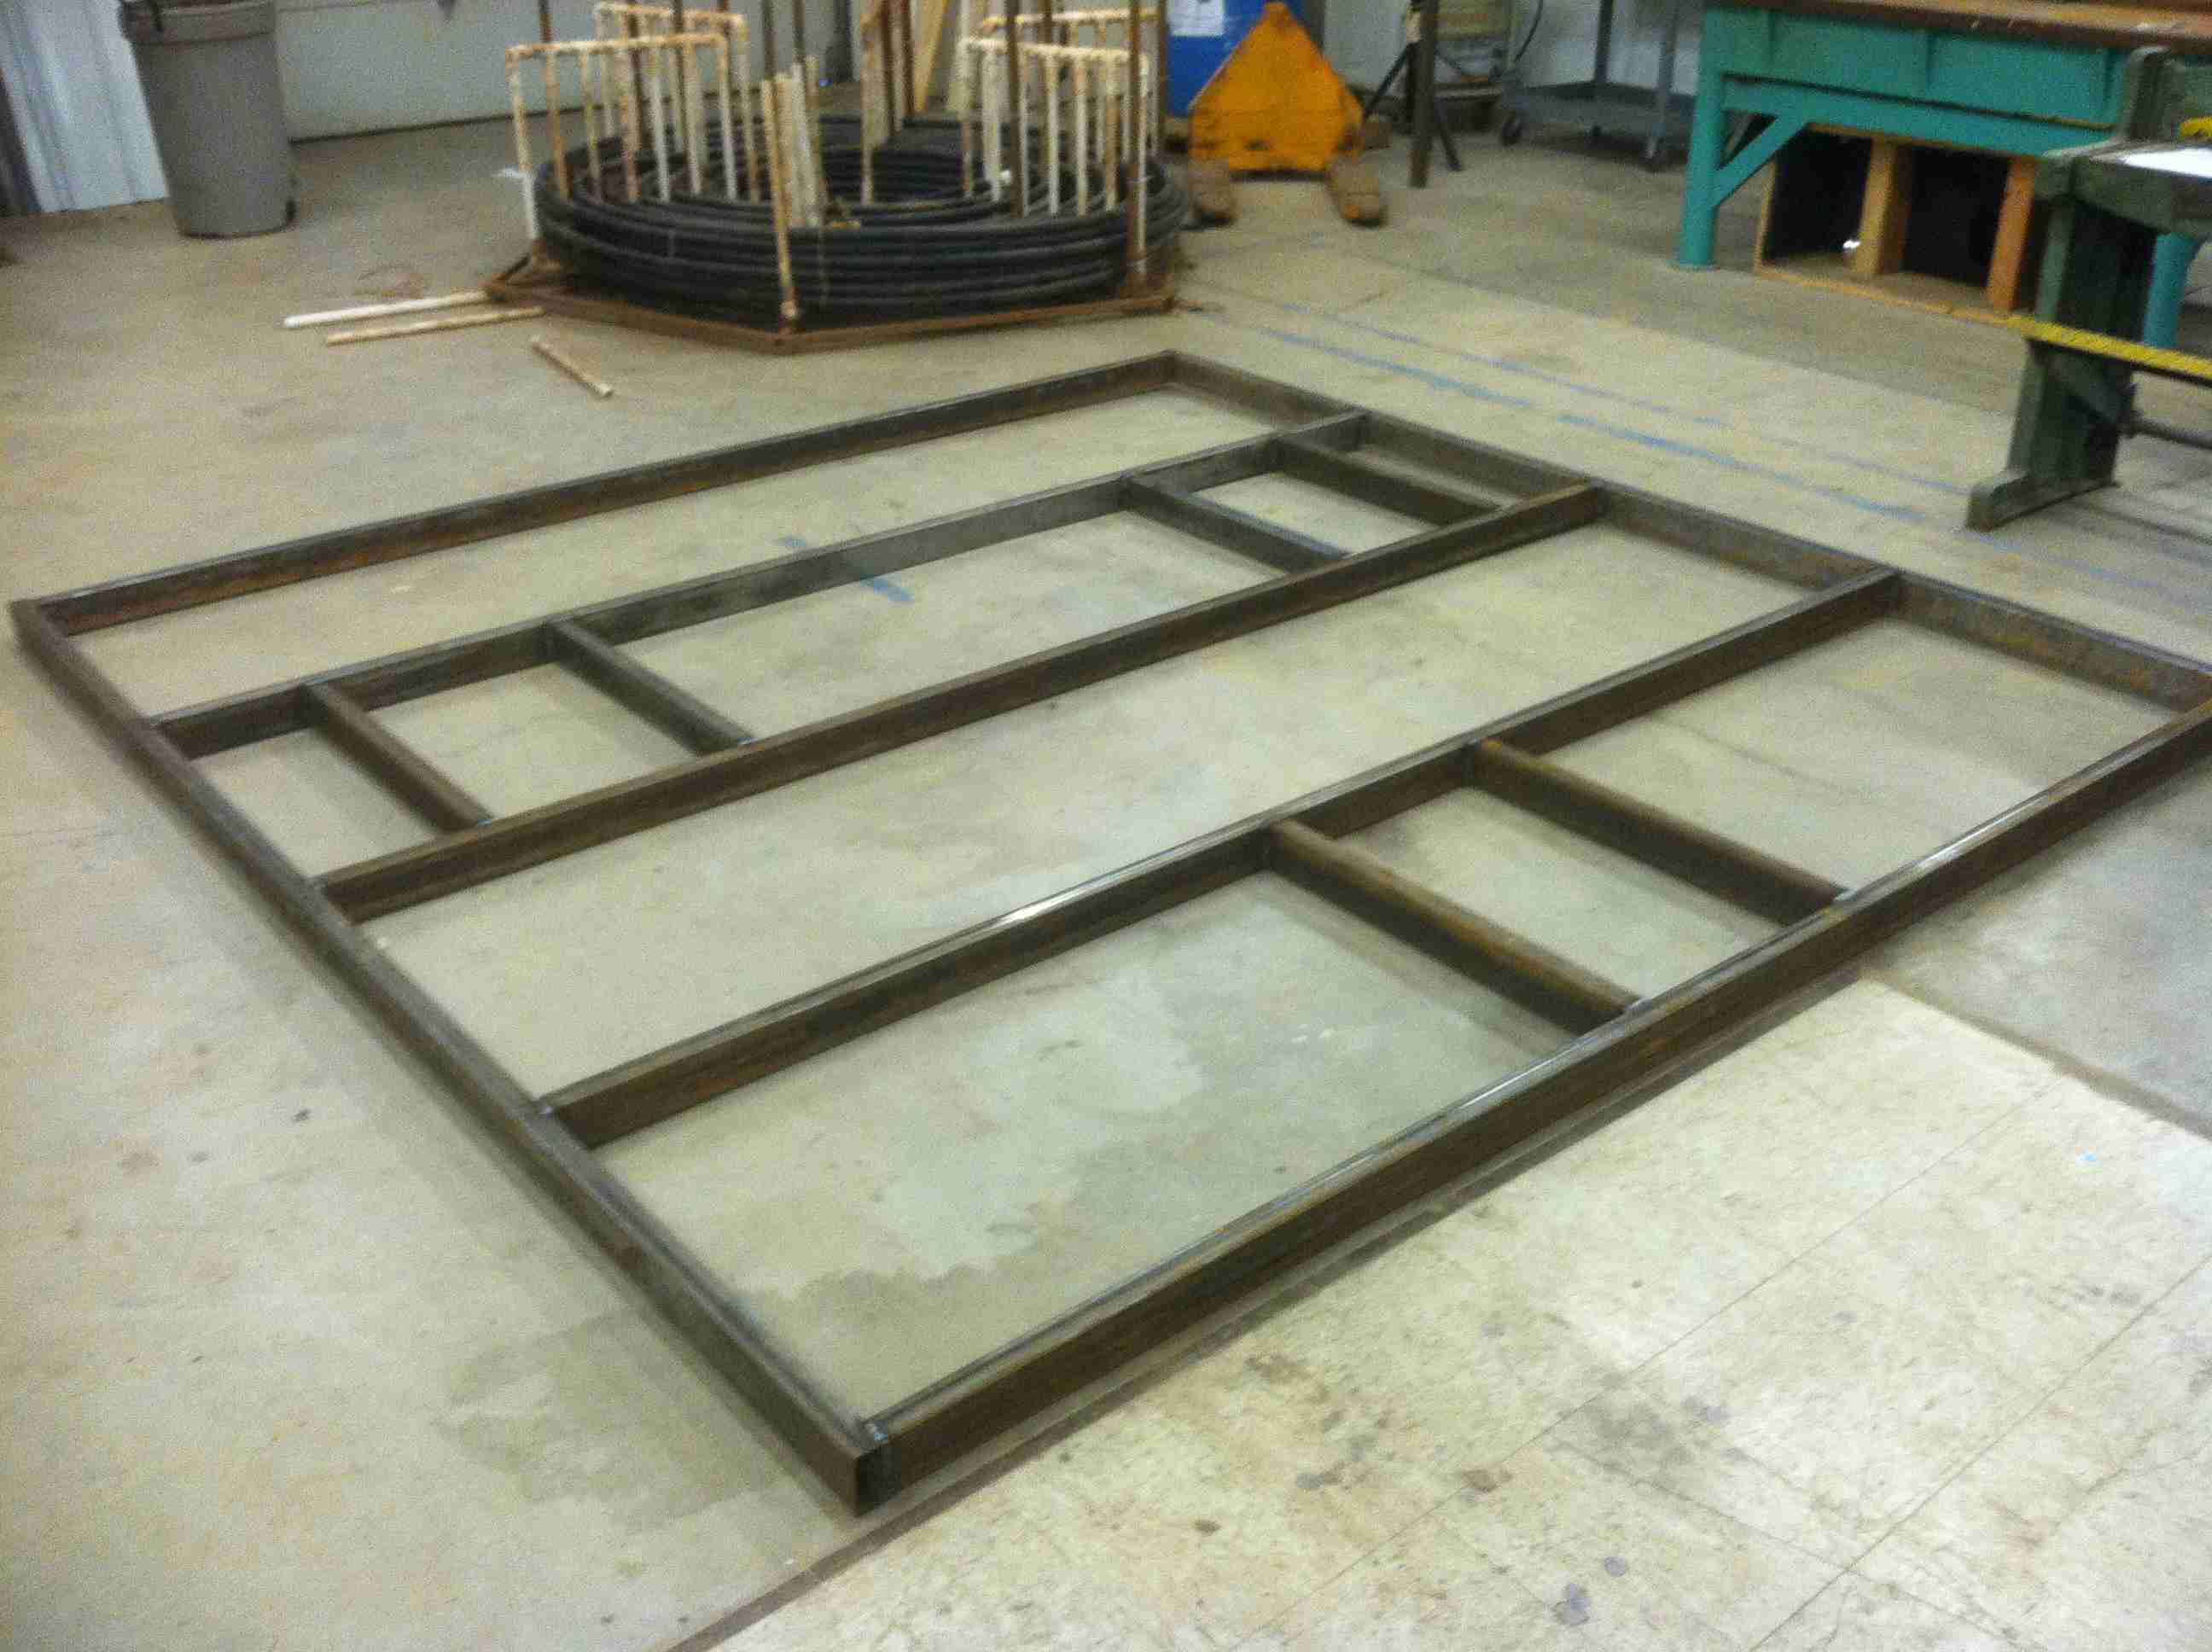
\includegraphics[width=0.8\textwidth]{Weighted_Frame.jpg}
		\caption[Weighted support frame]{Weighted support frame}
		\label{fig:ExpMethod:HeatExtr:Apparatus:WeightedFrame}
	\end{figure}

Three submersible load cells were connected between the weighted load cell frame and the SWHE support frame as can be seen in Figure \ref{fig:ExpMethod:HeatExtr:Apparatus:UWLoadCell}. Each load cell was capable of measuring 500 lb  (227 kg) in tension or compression. They were then connected together in parallel through as signal conditioning unit that would aggregate the total signal from the three load cells into one analog output signal which could be read by the data logger.

	\begin{figure}
		\centering
		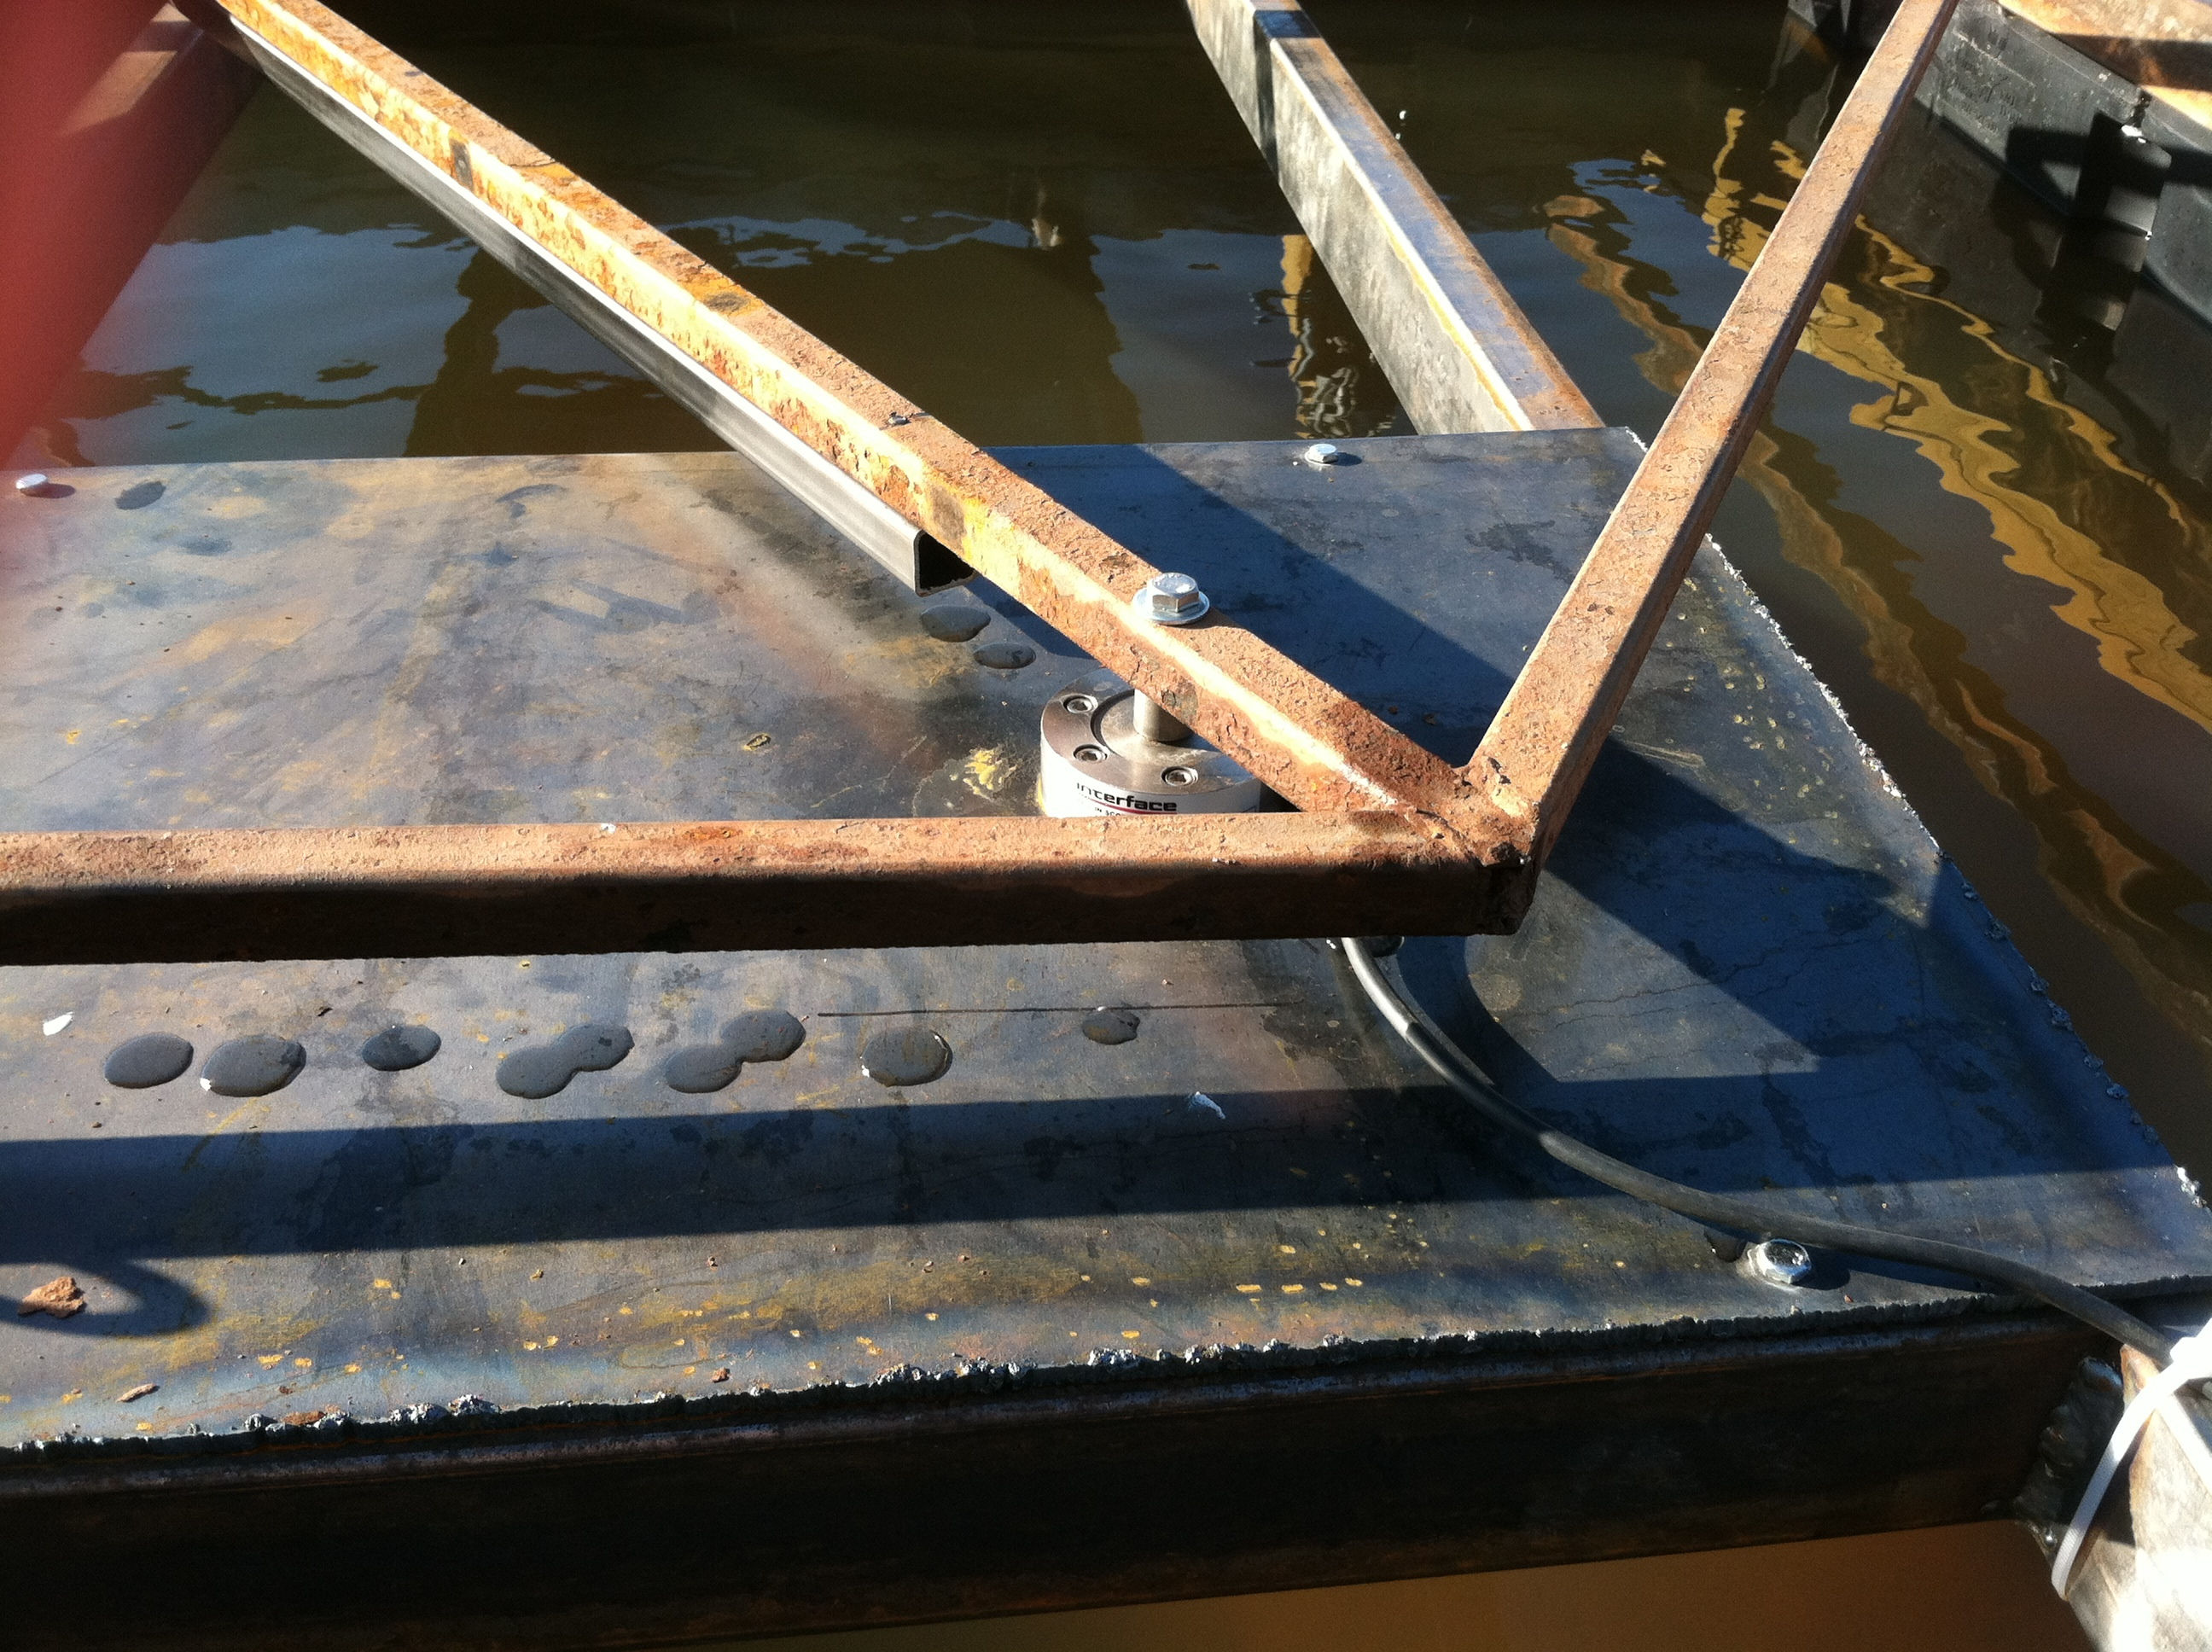
\includegraphics[width=0.8\textwidth]{Submersible_LoadCell.jpg}
		\caption[Submersible load cell]{Submersible load cell used to measure buoyancy force}
		\label{fig:ExpMethod:HeatExtr:Apparatus:UWLoadCell}
	\end{figure}

To support the weighted load cell frame, a support platform was constructed off site in segments and then brought to the test pond and assembled. The support platform can be seen in Figure \ref{fig:ExpMethod:HeatExtr:Apparatus:ExtrPlatformBuildMain}. The platform's intended purpose was to support the load cell frame from the water surface. It would allow for the load cell frame to be positioned in the pond, and then the SWHE lowered via four 500 lb (227 kg) capacity winches to the intended depth. The support platform's inside opening dimensions were 10 ft.\ x 10 ft.\ (3 x 3 m); outside dimensions were 14 ft.\ x 14 ft.\ (4.3 x 4.3 m). The platform was supported by 10, 2 ft.\ (61 cm) wide by 4 ft.\ (122 cm) long by 1 ft.\ (30.5 cm) deep HDPE coated Styrofoam dock floats. The 10 dock floats had a combined buoyancy capacity of approximately 2000 lb (907 kg) floating 6 in.\ (15 cm) above the water. The final testing platform can be see in Figure \ref{fig:ExpMethod:HeatExtr:Apparatus:ExtrPlatformFinal}. A schematic representation of the support platform can be seen in Figure \ref{fig:ExpMethod:HeatExtr:Apparatus:ExtrExpPondSchematic}.

While performing experiments in the pond with this apparatus, the thermistors measuring pond temperature were placed on the cables supporting the load cell frame. They were placed at a distance of approximately 4 ft.\ (1.2 m) away from the SWHE. Surface water temperature was determined as shown in Equation \ref{eq:ExpMethod:HeatRej:Apparatus:PondTemp}.

	\begin{figure}
		\centering
		\subfloat[First segment of ice-on-coil platform.]{
			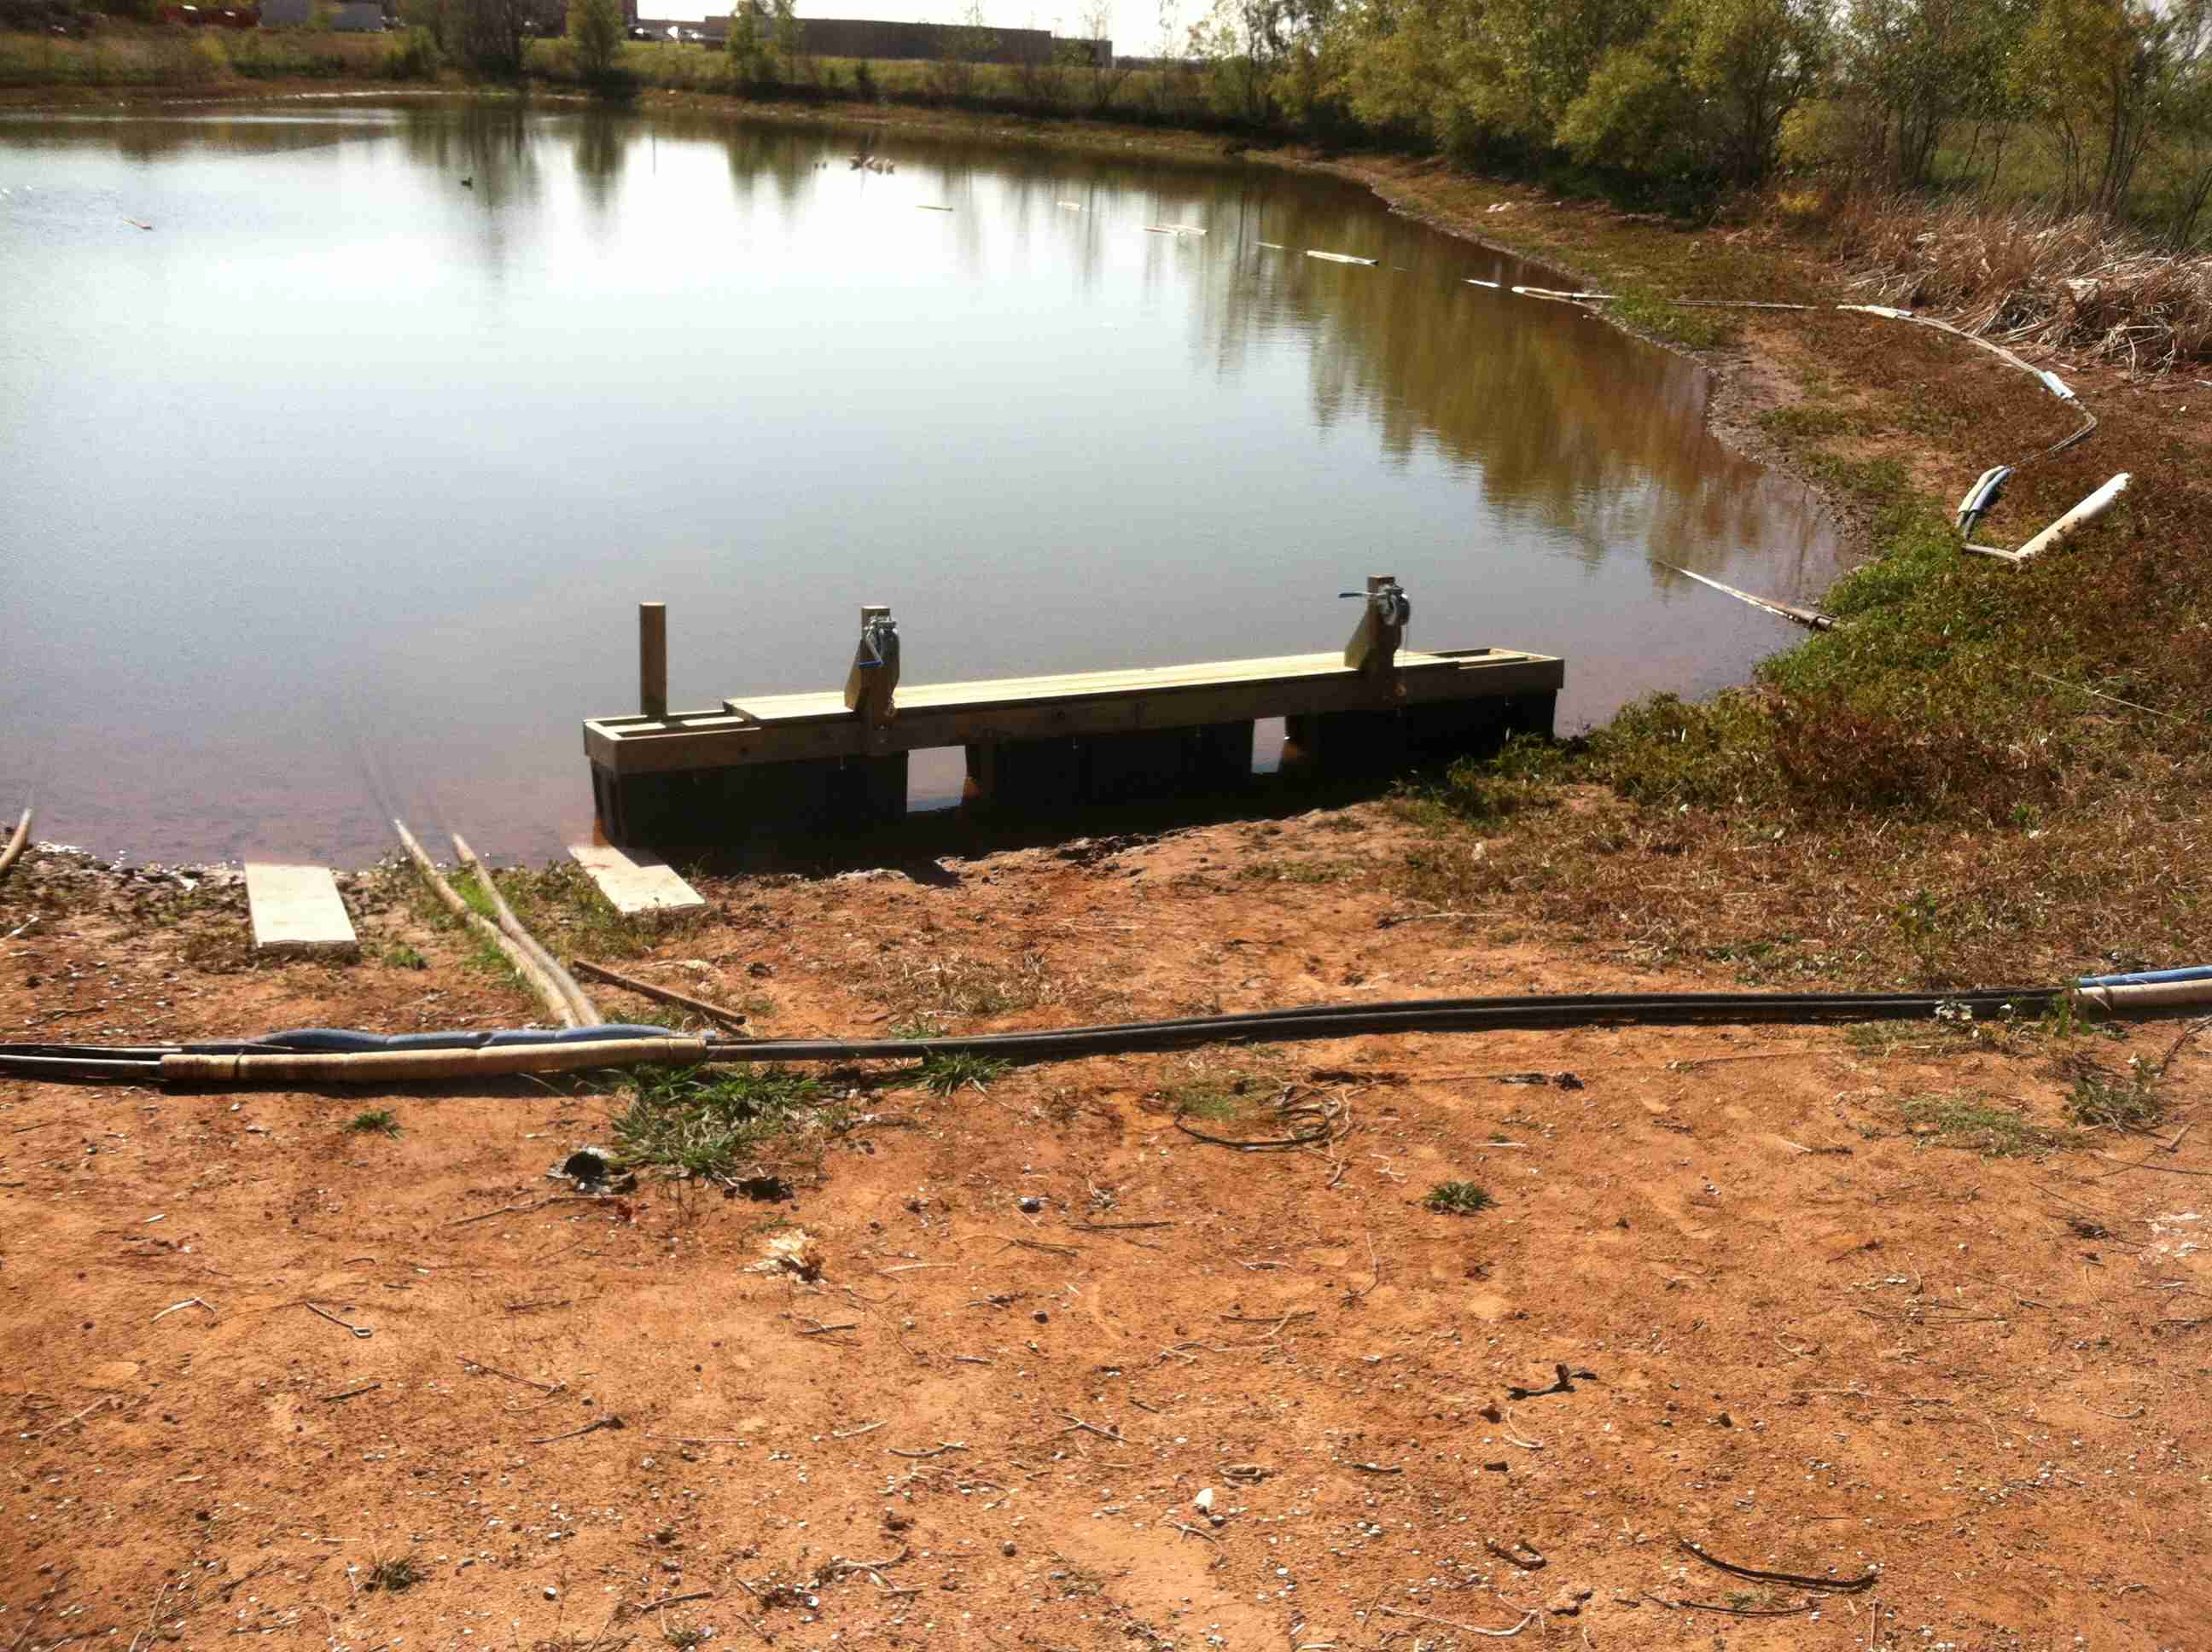
\includegraphics[width=0.47\textwidth]{Extr_Platform_Build1.jpg}
			\label{fig:ExpMethod:HeatExtr:Apparatus:ExtrPlatformBuild1}}
		\,
		\subfloat[Second segment of ice-on-coil platform.]{
			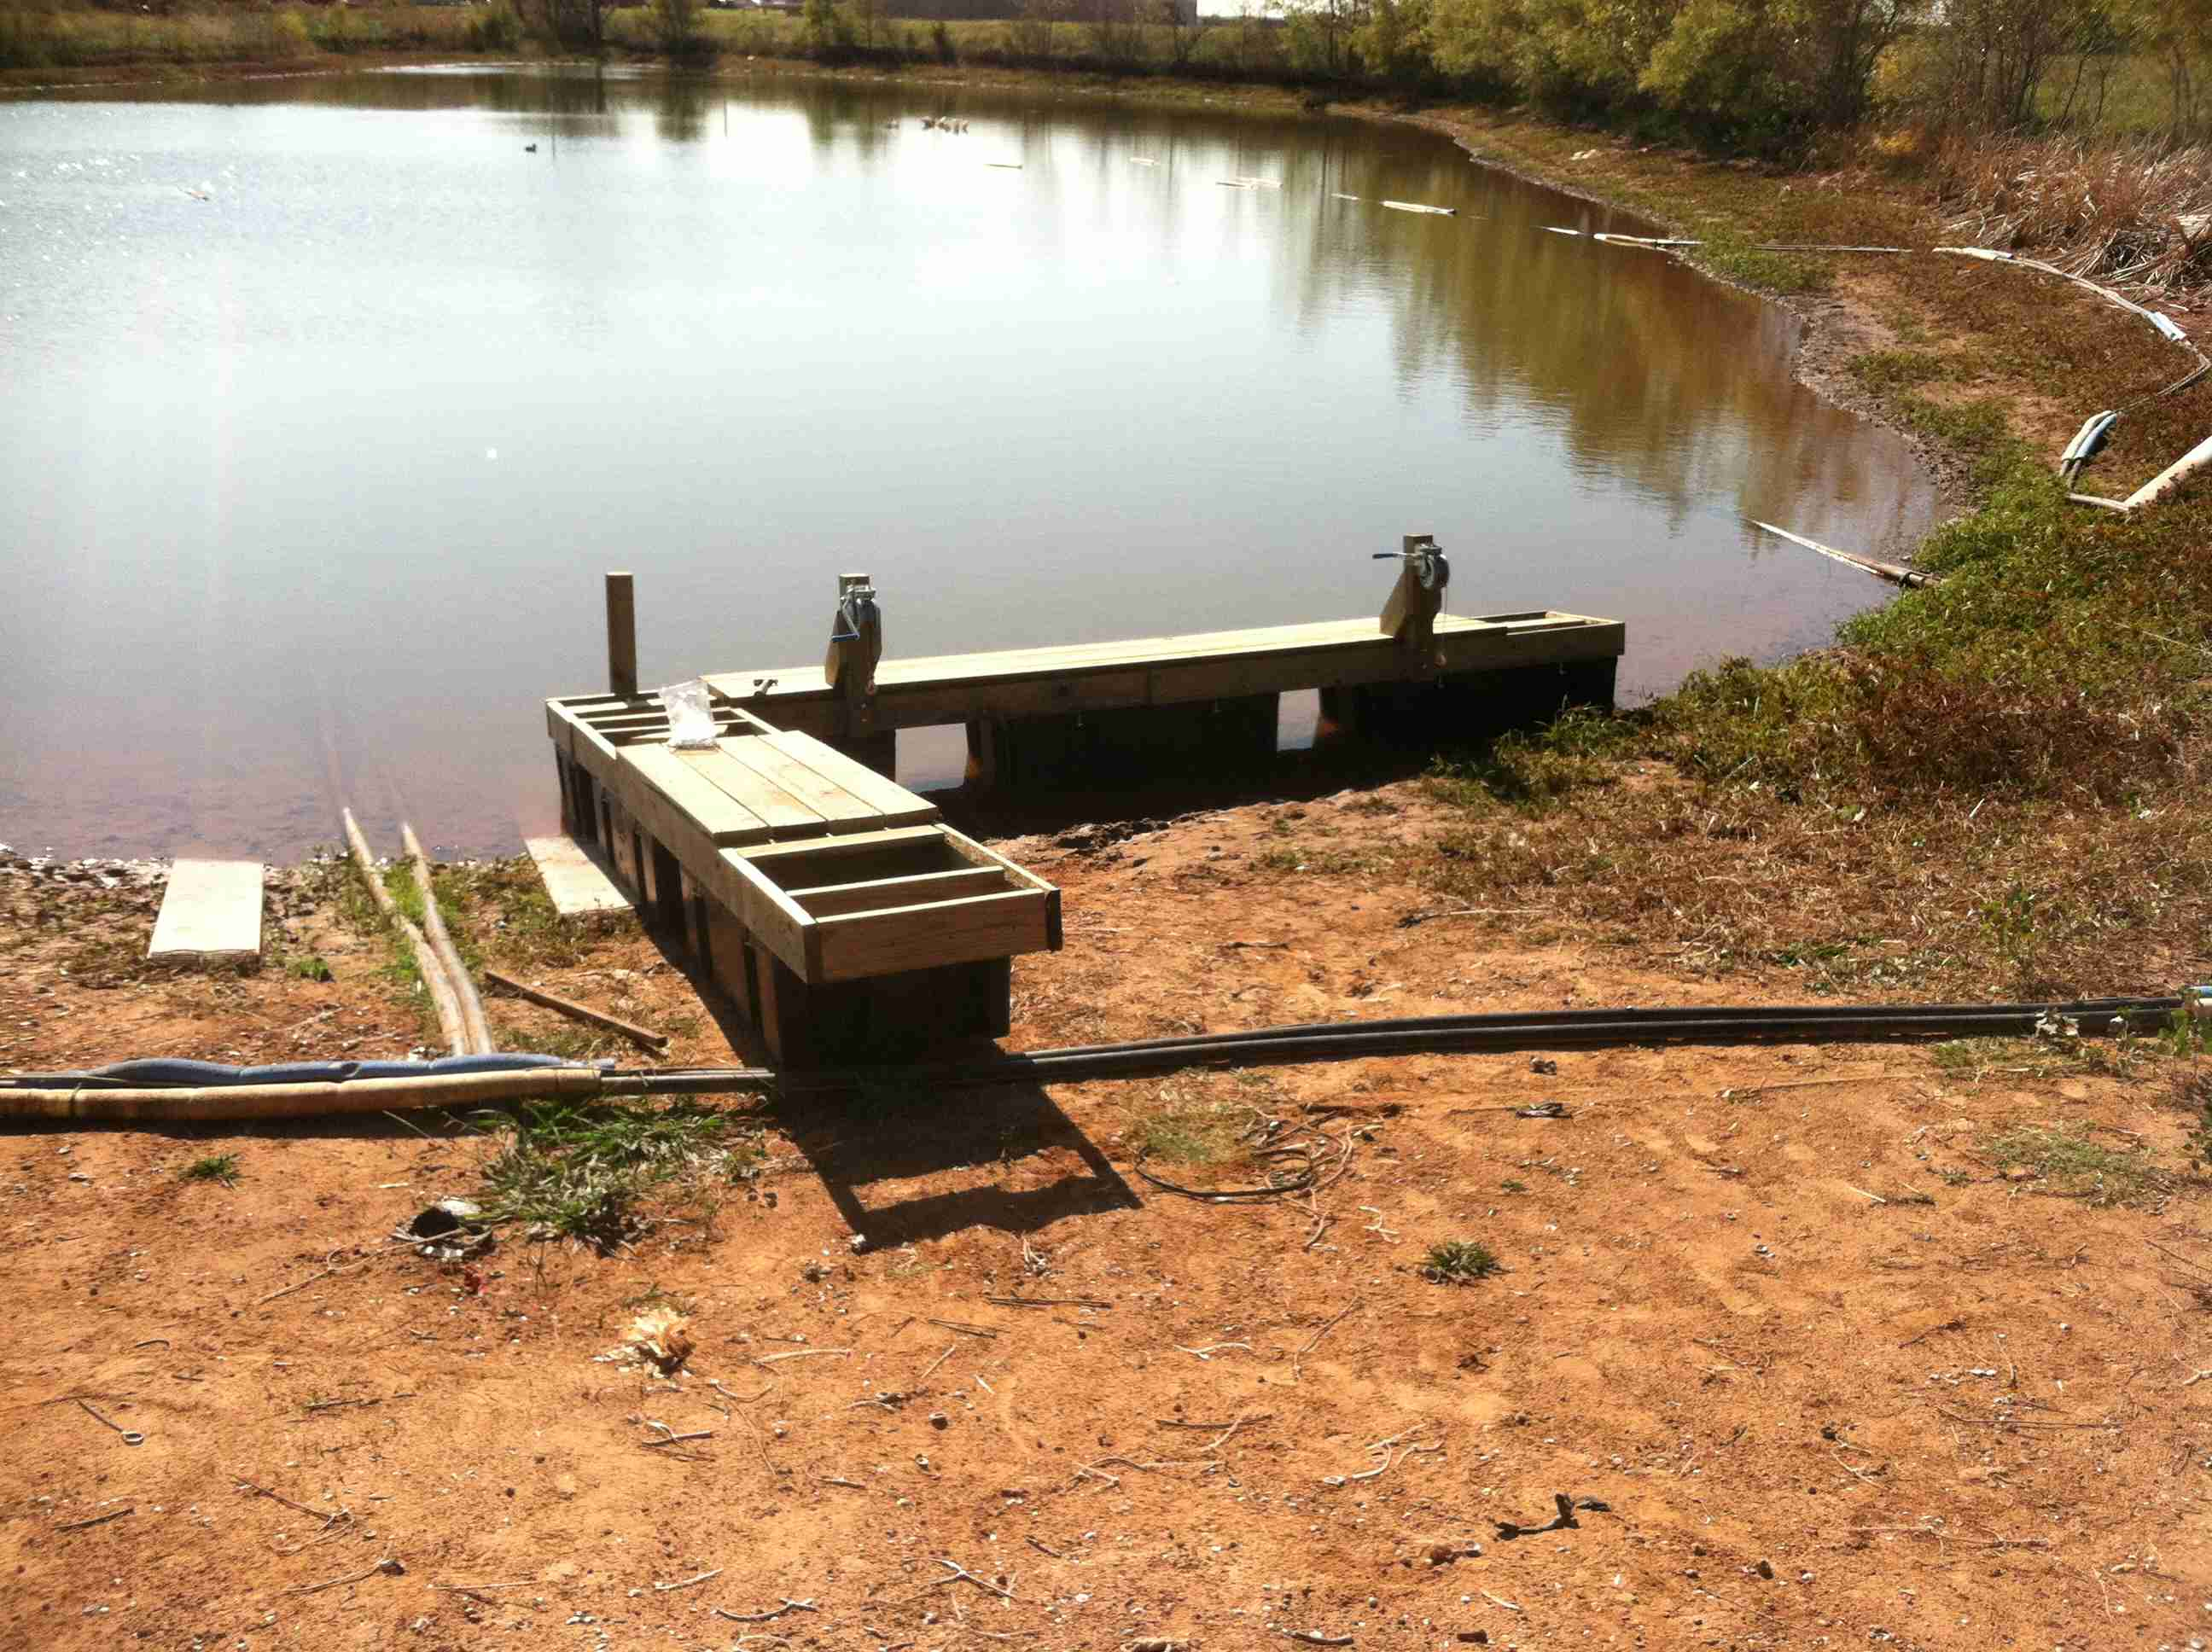
\includegraphics[width=0.47\textwidth]{Extr_Platform_Build2.jpg}
			\label{fig:ExpMethod:HeatExtr:Apparatus:ExtrPlatformBuild2}}
		\\
		\subfloat[Third segment of ice-on-coil platform.]{
			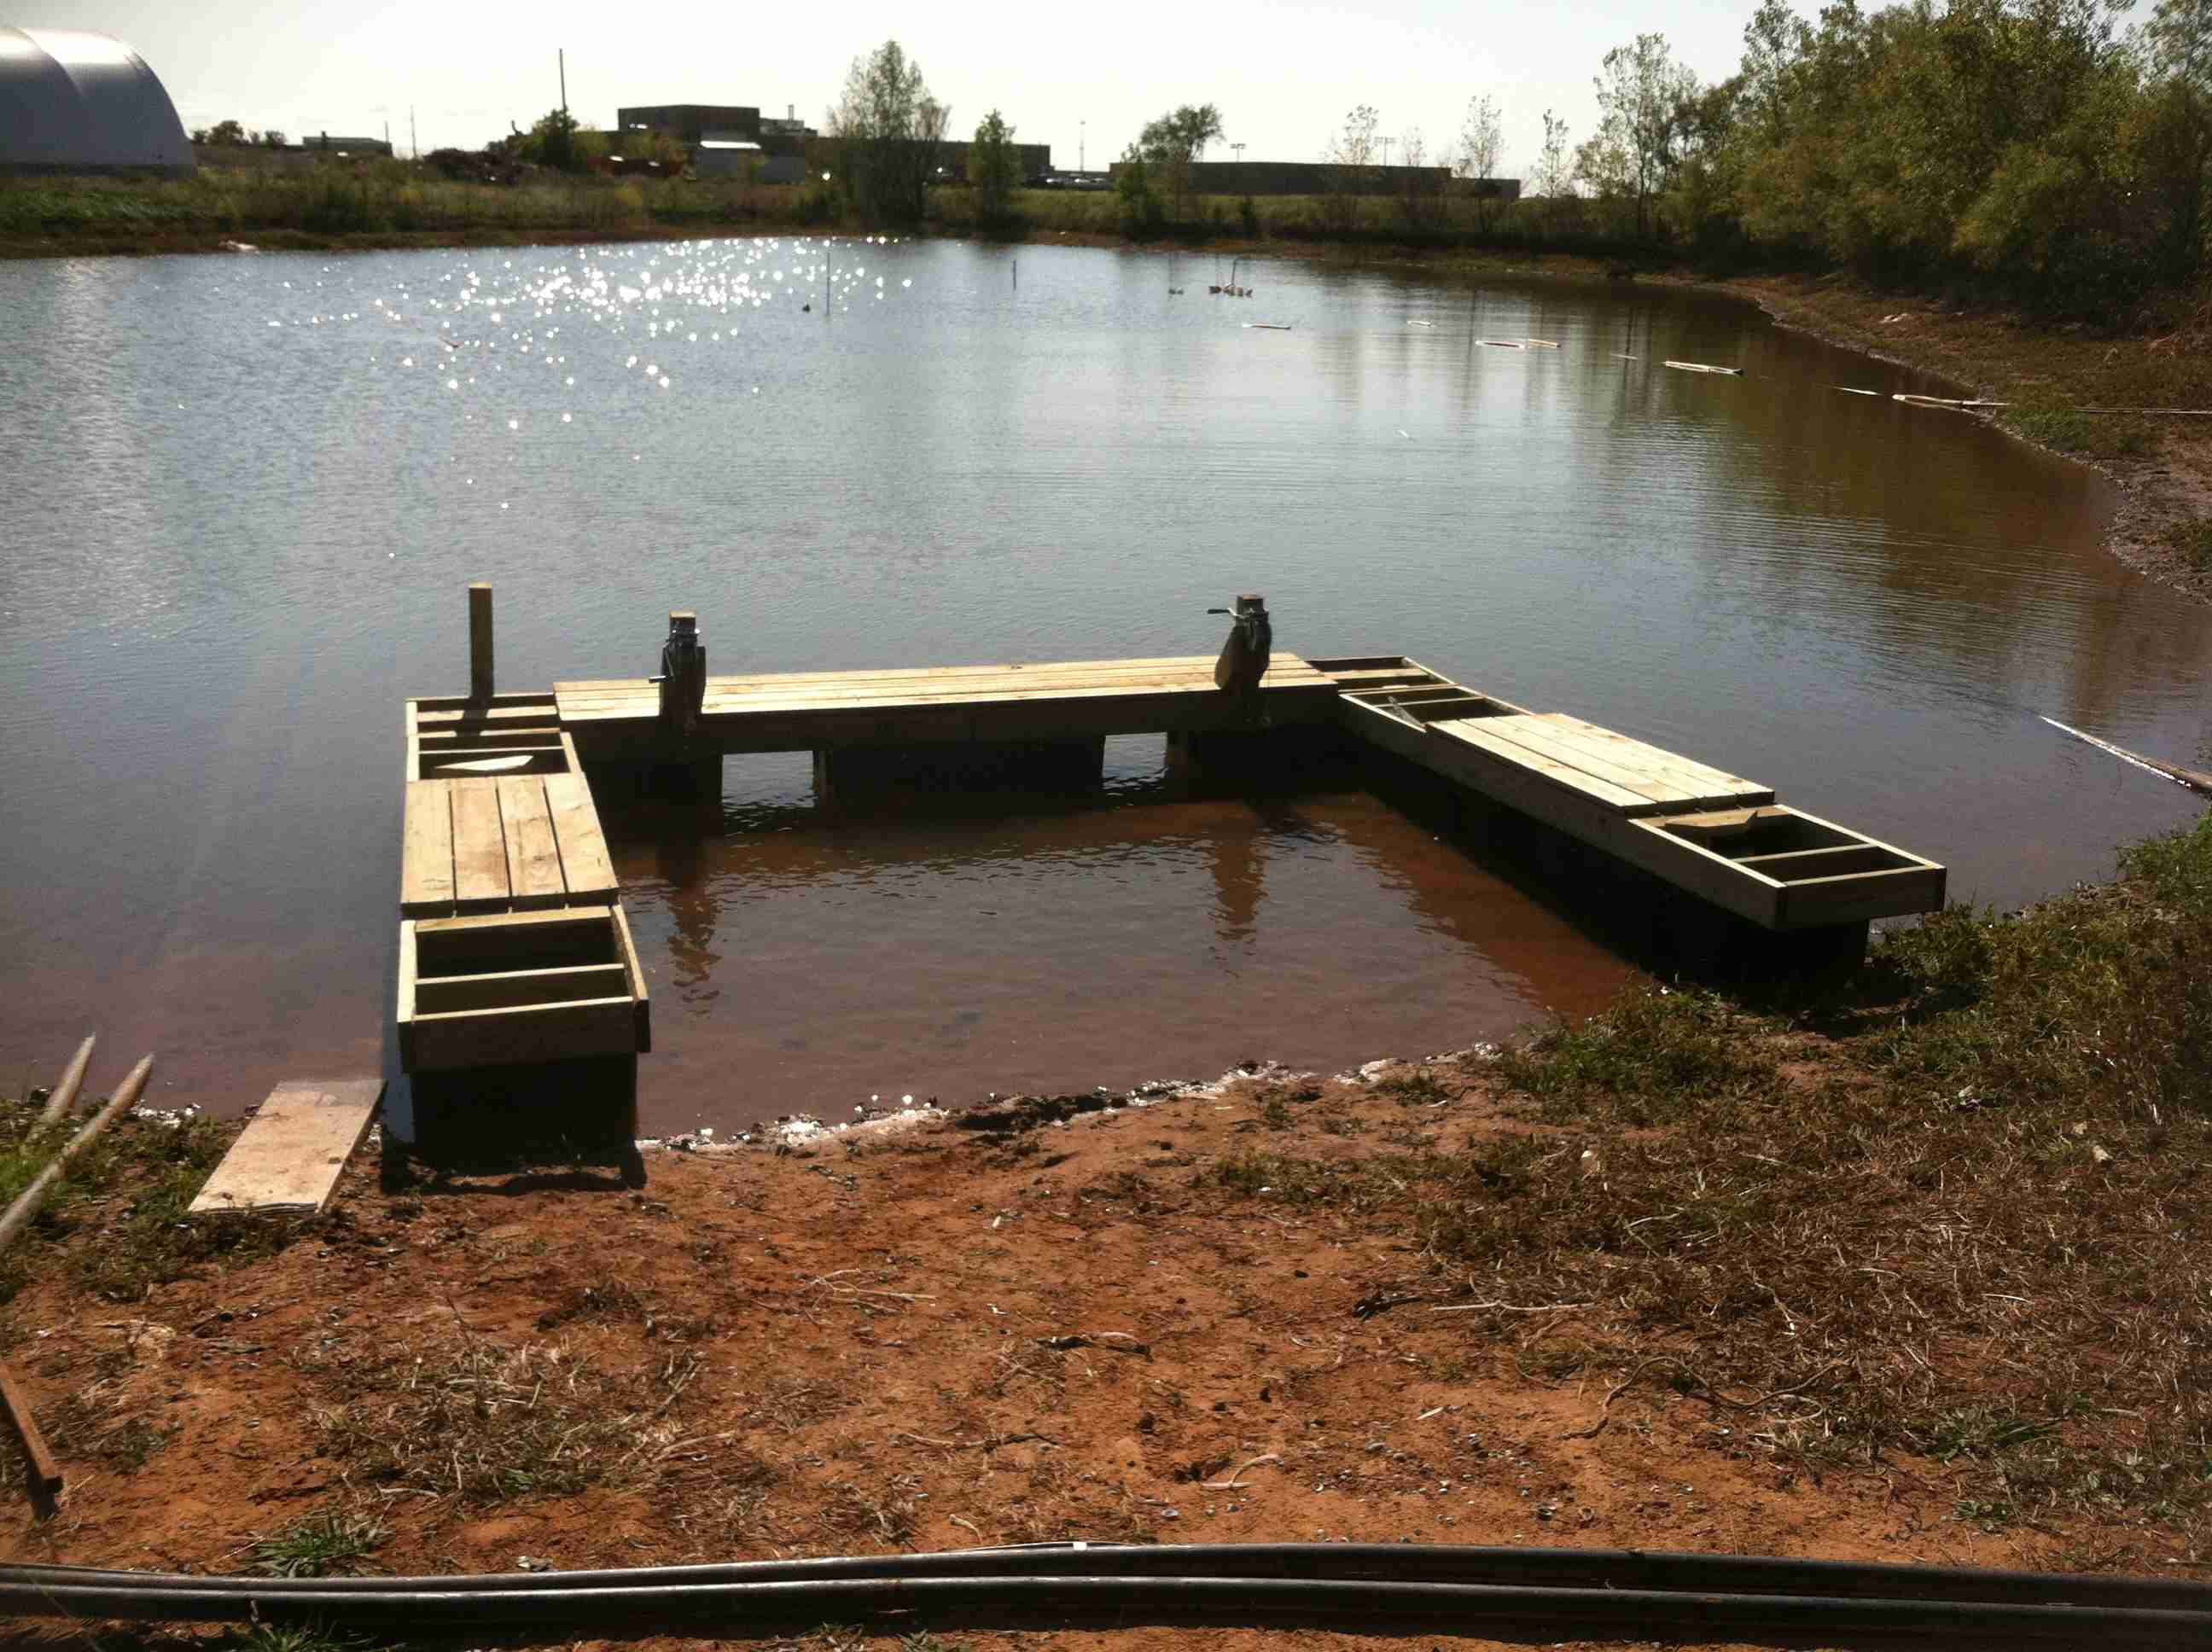
\includegraphics[width=0.47\textwidth]{Extr_Platform_Build3.jpg}
			\label{fig:ExpMethod:HeatExtr:Apparatus:ExtrPlatformBuild3}}
		\,
		\subfloat[Final ice-on-coil platform.]{
			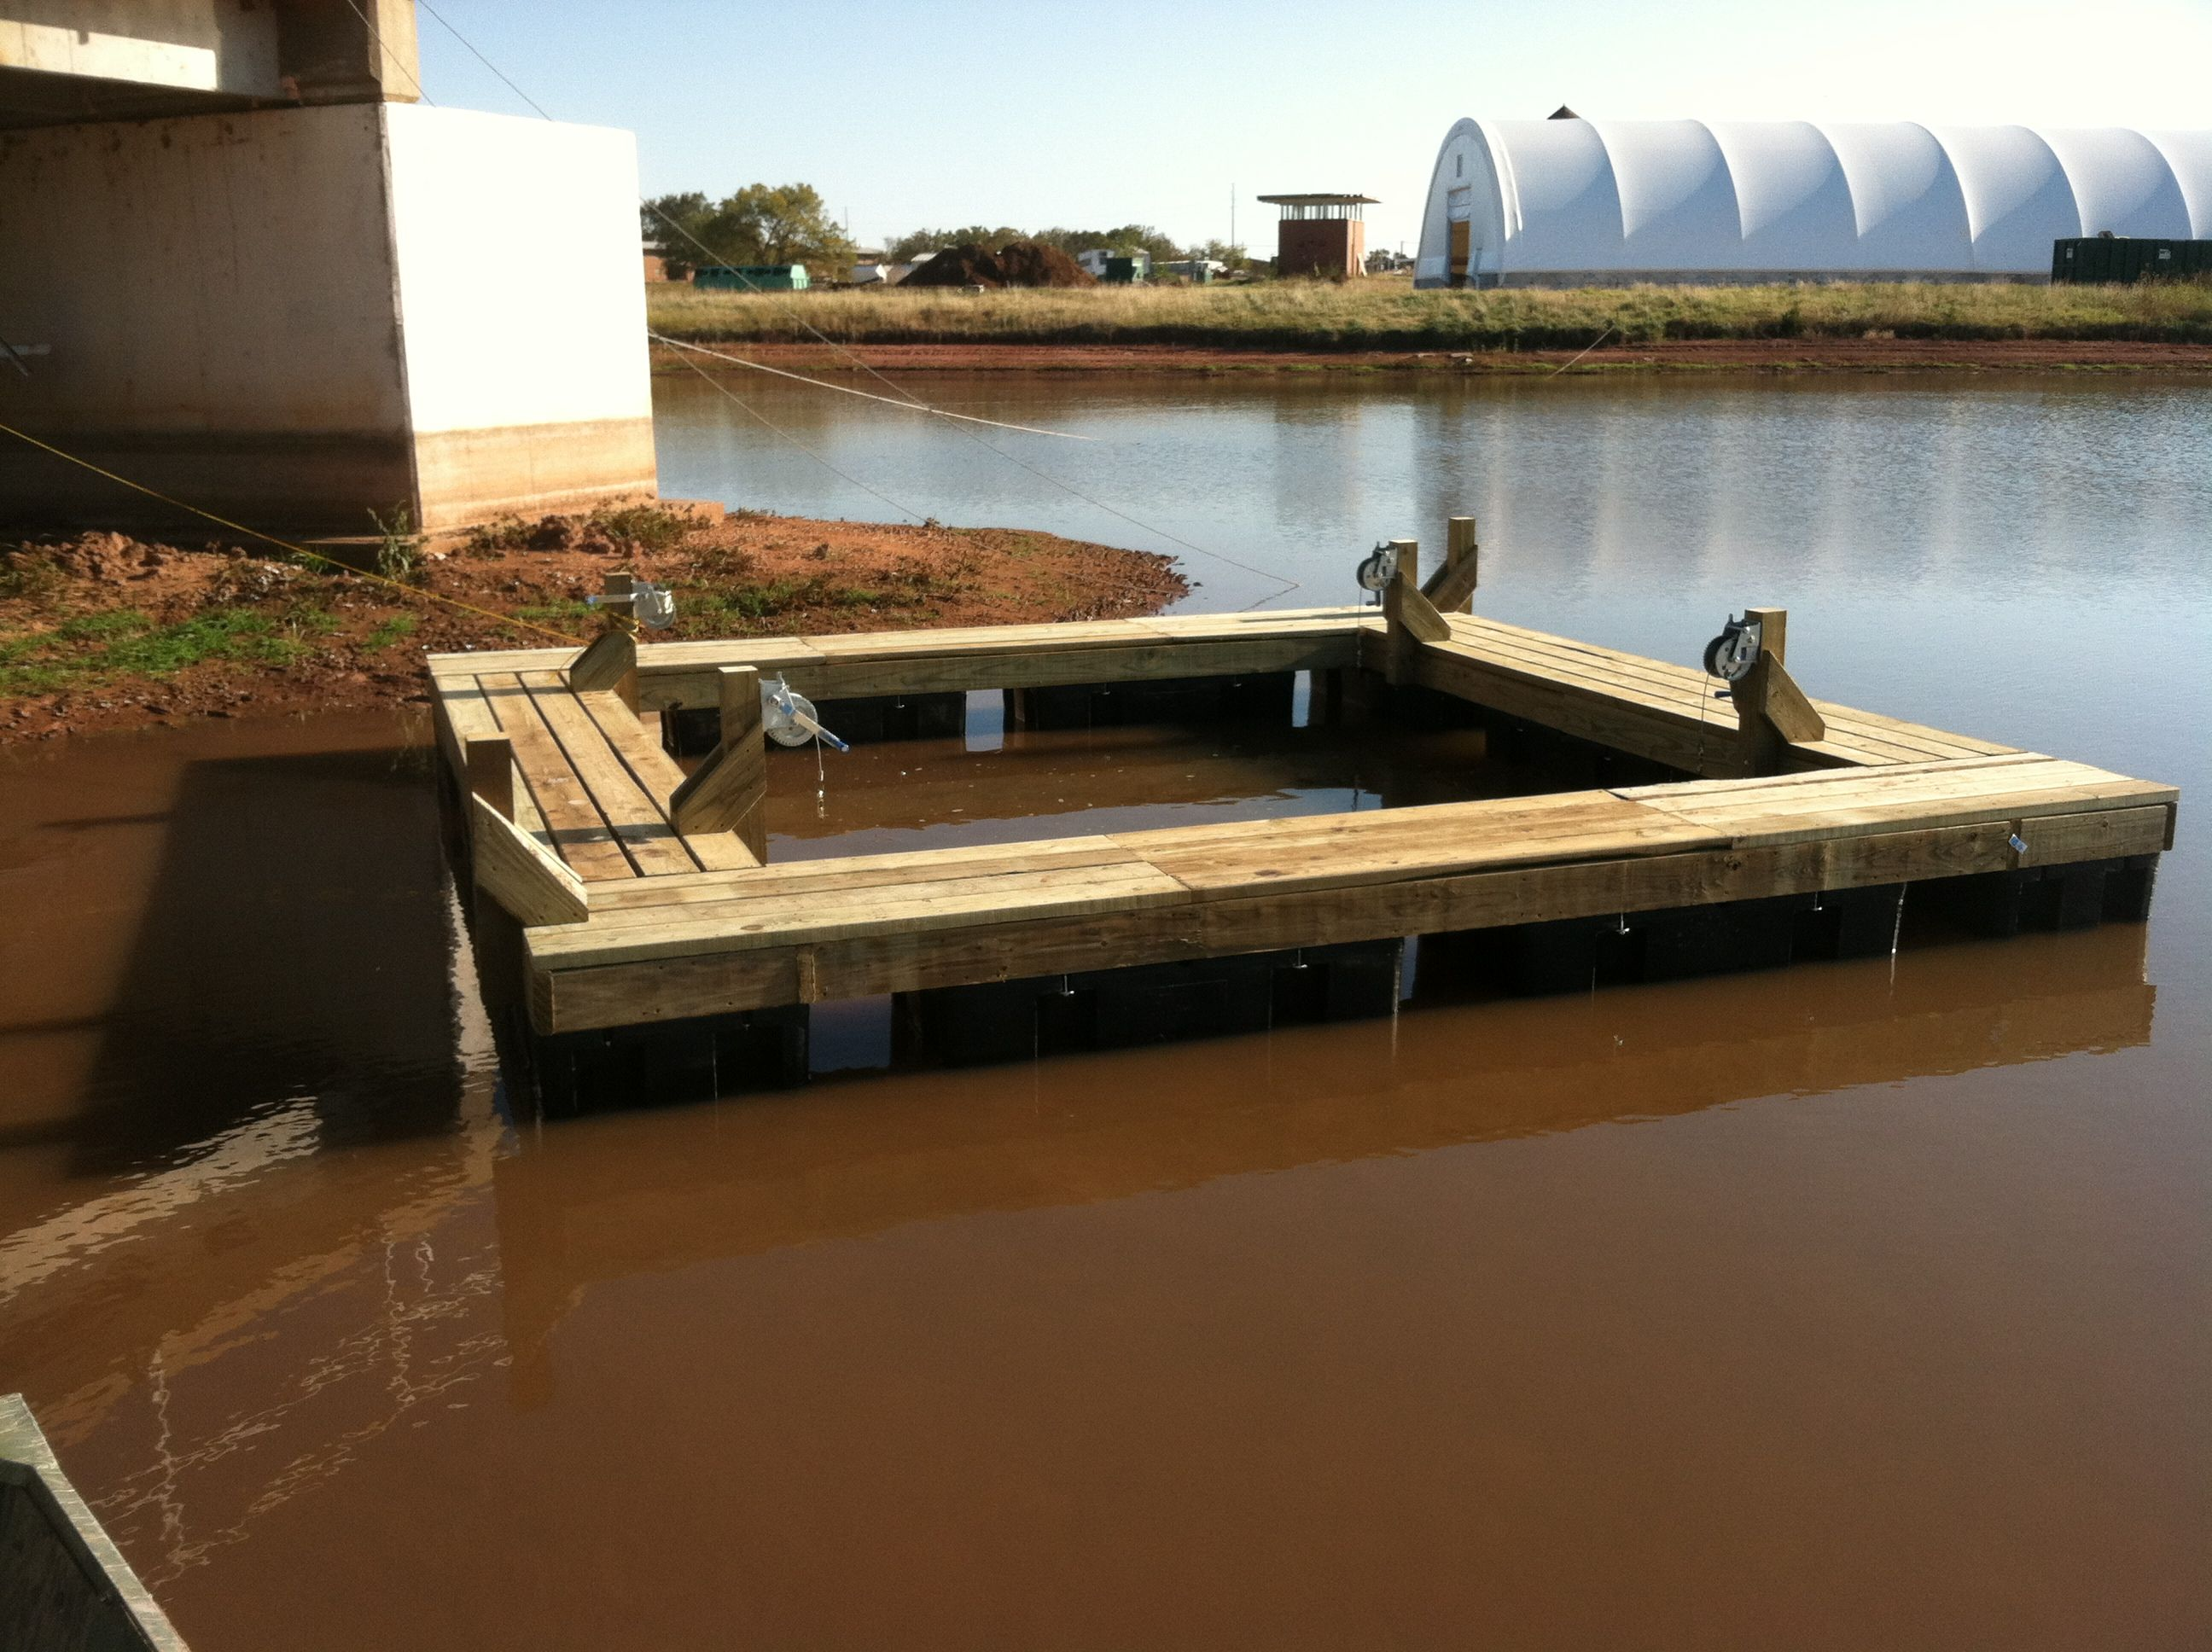
\includegraphics[width=0.47\textwidth]{Extr_Platform_Build4.jpg}
			\label{fig:ExpMethod:HeatExtr:Apparatus:ExtrPlatformBuild4}}
		\caption[Construction of ice-on-coil platform]{Construction of ice-on-coil platform}
		\label{fig:ExpMethod:HeatExtr:Apparatus:ExtrPlatformBuildMain}
	\end{figure}

	\begin{figure}
		\centering
		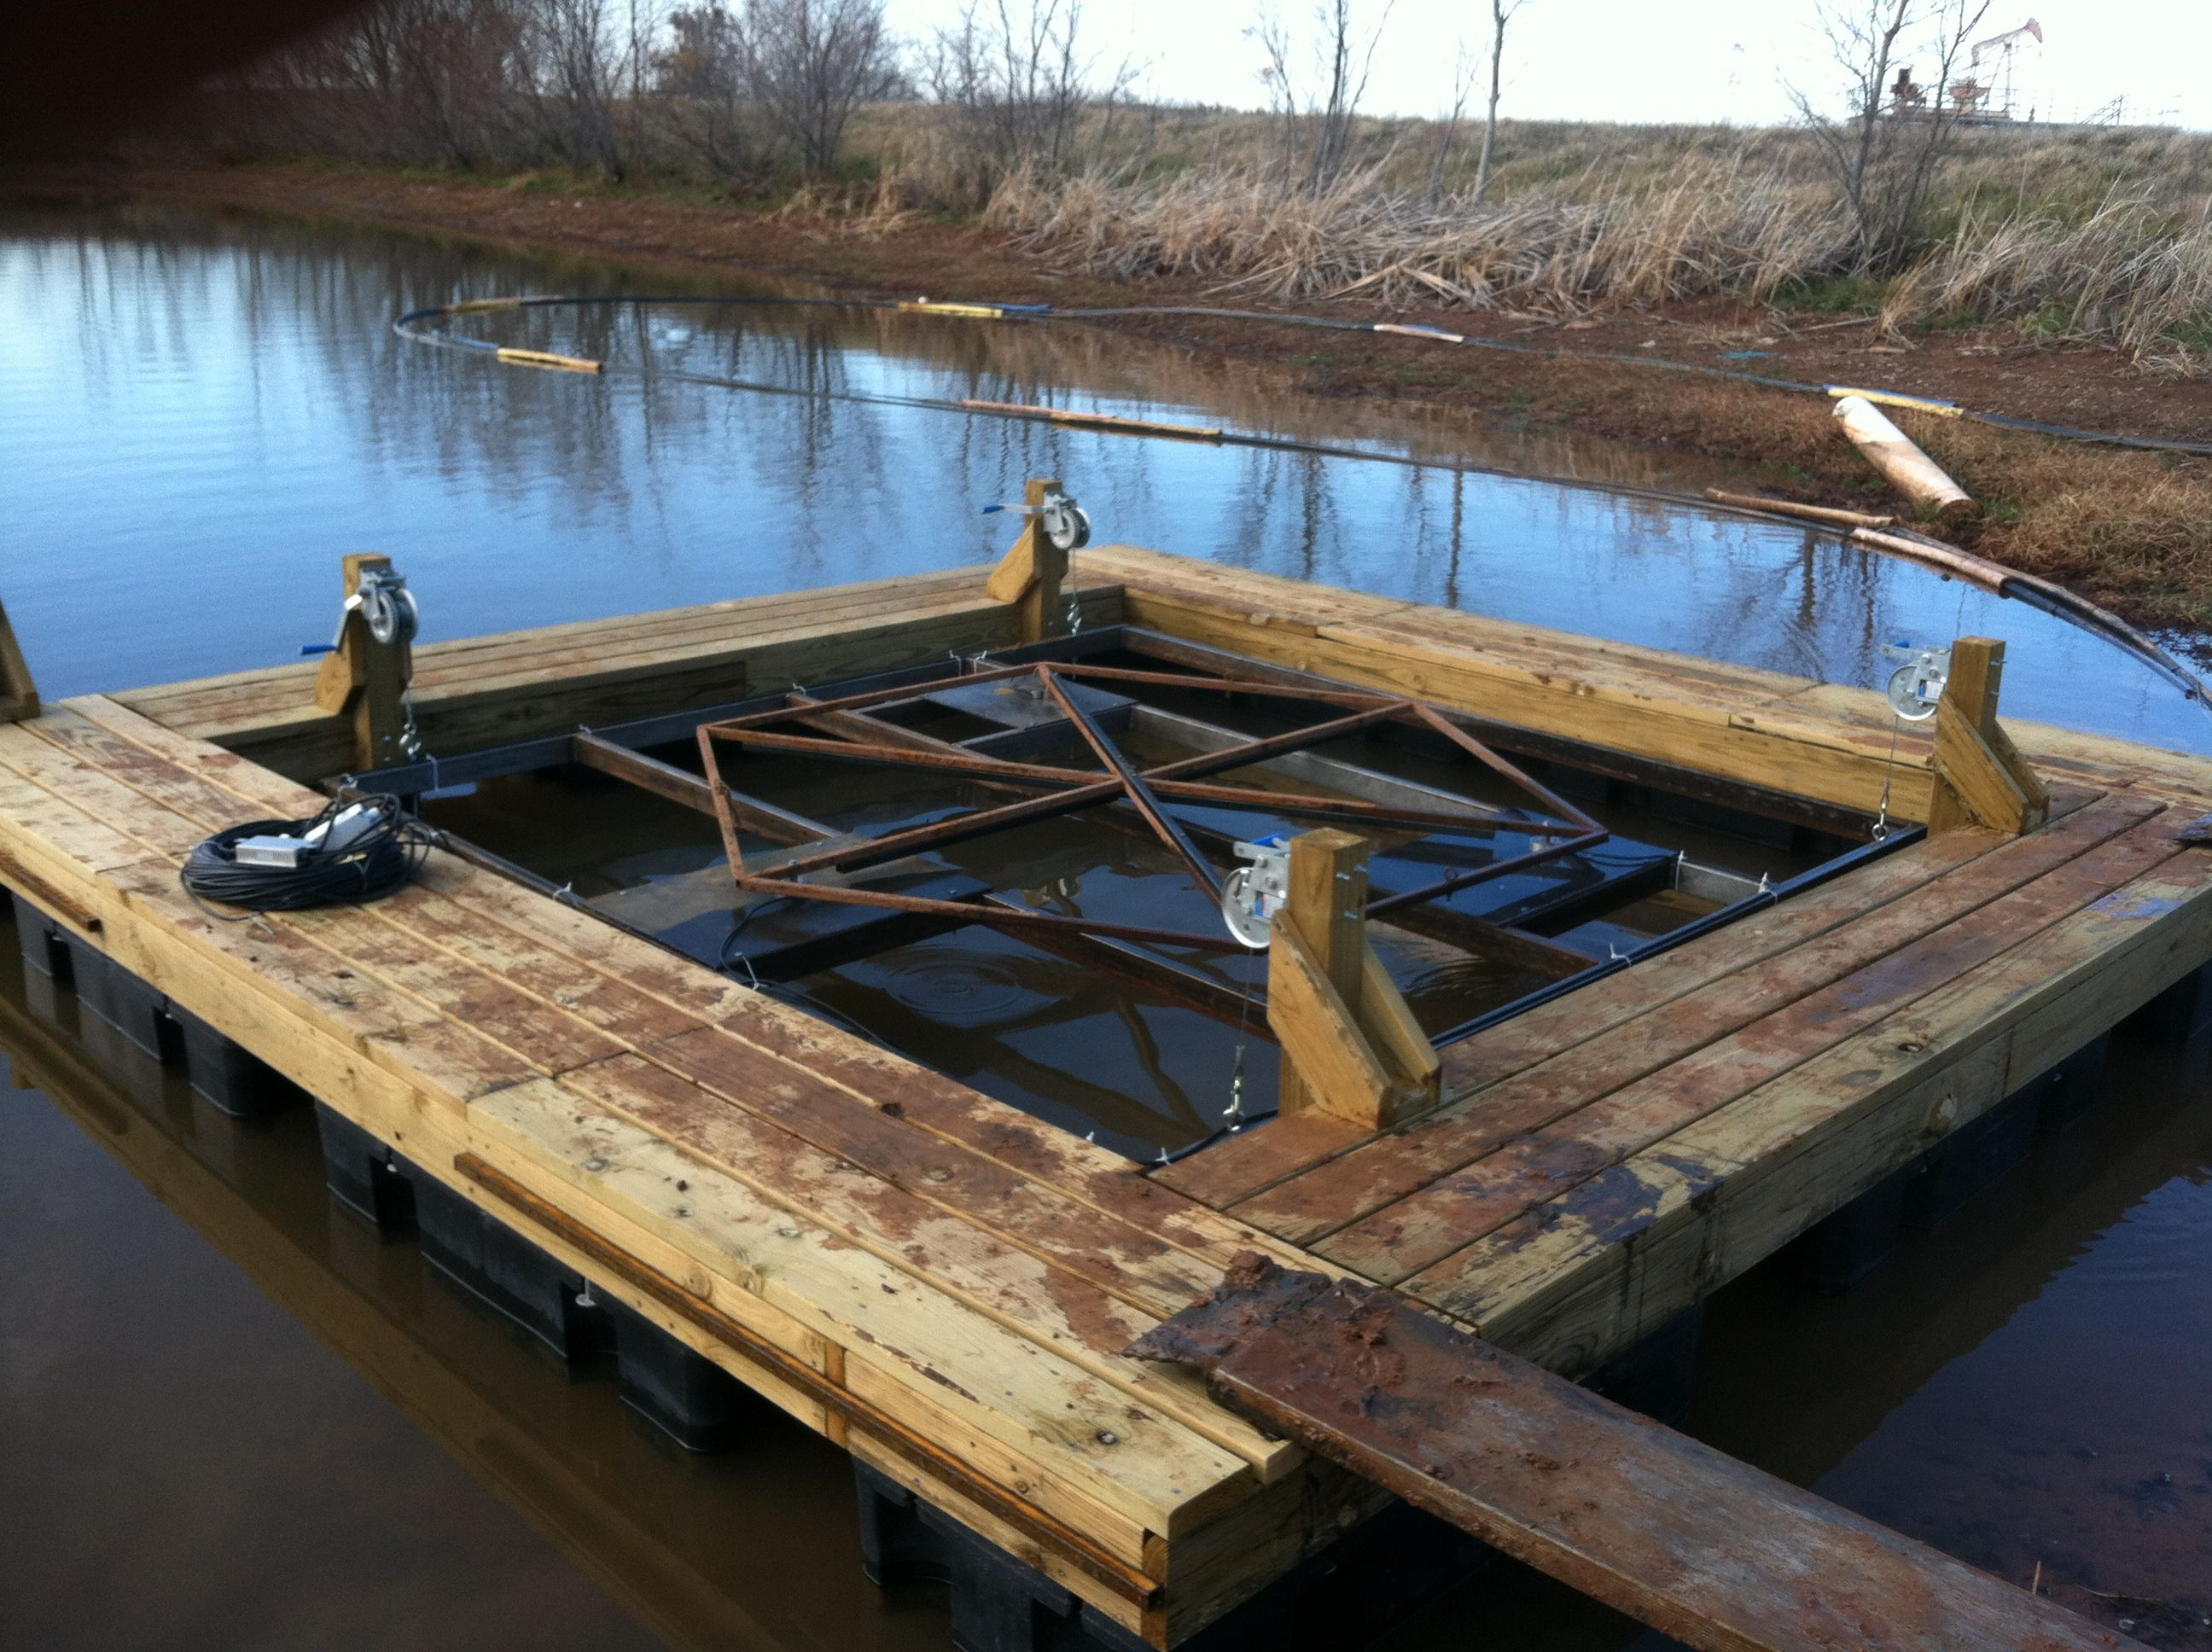
\includegraphics[width=0.8\textwidth]{Extr_Platform_Final.jpg}
		\caption[Final ice-on-coil platform]{Heat extraction experiment support platform and load cell frame}
		\label{fig:ExpMethod:HeatExtr:Apparatus:ExtrPlatformFinal}
	\end{figure}


	\begin{figure}
		\centering
		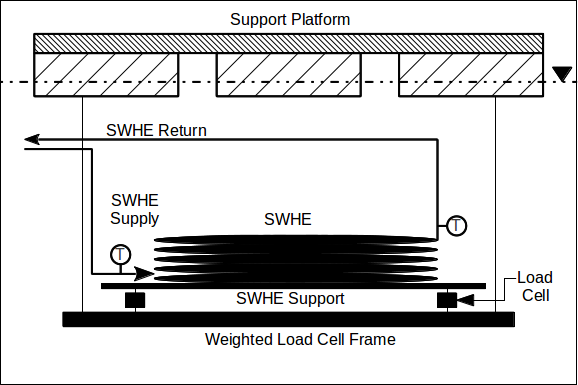
\includegraphics[width=0.8\textwidth]{SWHE_Ext_Pond.png}
		\caption[Schematic of heat extraction equipment in pond]{Schematic of heat extraction equipment in pond}
		\label{fig:ExpMethod:HeatExtr:Apparatus:ExtrExpPondSchematic}
	\end{figure}

Because heat was being extracted from the SWHE via the reversible heat pumps, the heat extracted by the 3 ton (10.6 kW) water-water heat pump was dissipated via another SWHE in a configuration identical to the one shown in Figure \ref{fig:ExpMethod:HeatRej:Apparatus:RejExpPond}. This additional SWHE was submerged in the test pond at a distance of roughly 100 ft away from the SWHE being tested. The additional SWHE was connected to the water-water heat pump via the ports labeled GHX in Figure \ref{fig:ExpMethod:HeatExtr:Apparatus:ExtrExpTrailerSchematic}.

As the weather and the test pond warmed, it became impossible with the current experiment to extract sufficient heat so as to cause ice to form on the SWHE. To allow continued heat extraction testing with the possibility of SWHE ice formation, the experiment was then moved to the indoor test facility.

To run tests indoors, a 4 ft.\ (1.2 m) deep by 15 ft.\ (4.6 m) diameter above ground pool was purchased and setup in the laboratory facility. The pool can be seen in Figure \ref{fig:ExpMethod:HeatExtr:Apparatus:EmptyPool}. The pool was constructed on top of 1/2 in.\ (12.7 mm) of extruded polystyrene foam (i.e. blue board) which has an R-Value of approximately 2.5 hr-ft$^2$-$^\circ$F/BTU (0.44 $m^2$-$^\circ C/W$). This was placed under the pool to reduce the amount of heat gain/loss to the pool while running experiments. The perimeter of the pool was also insulated with R-13 (2.3 $m^2$-$^\circ C/W$)fiber-glass batt insulation. The pool can be seen half insulated in Figure \ref{fig:ExpMethod:HeatExtr:Apparatus:FullPool}. Heat extracted from the pool via the SWHE was then rejected via the heat pumps to the lab space for the water-air heat pump, and to two vertical borehole ground heat exchangers whose connections were inside the lab space for the water-water heat pump. The connections to these ground heat exchangers can be seen in Figure \ref{fig:ExpMethod:HeatExtr:Apparatus:GHX}.

	\begin{figure}
		\centering
		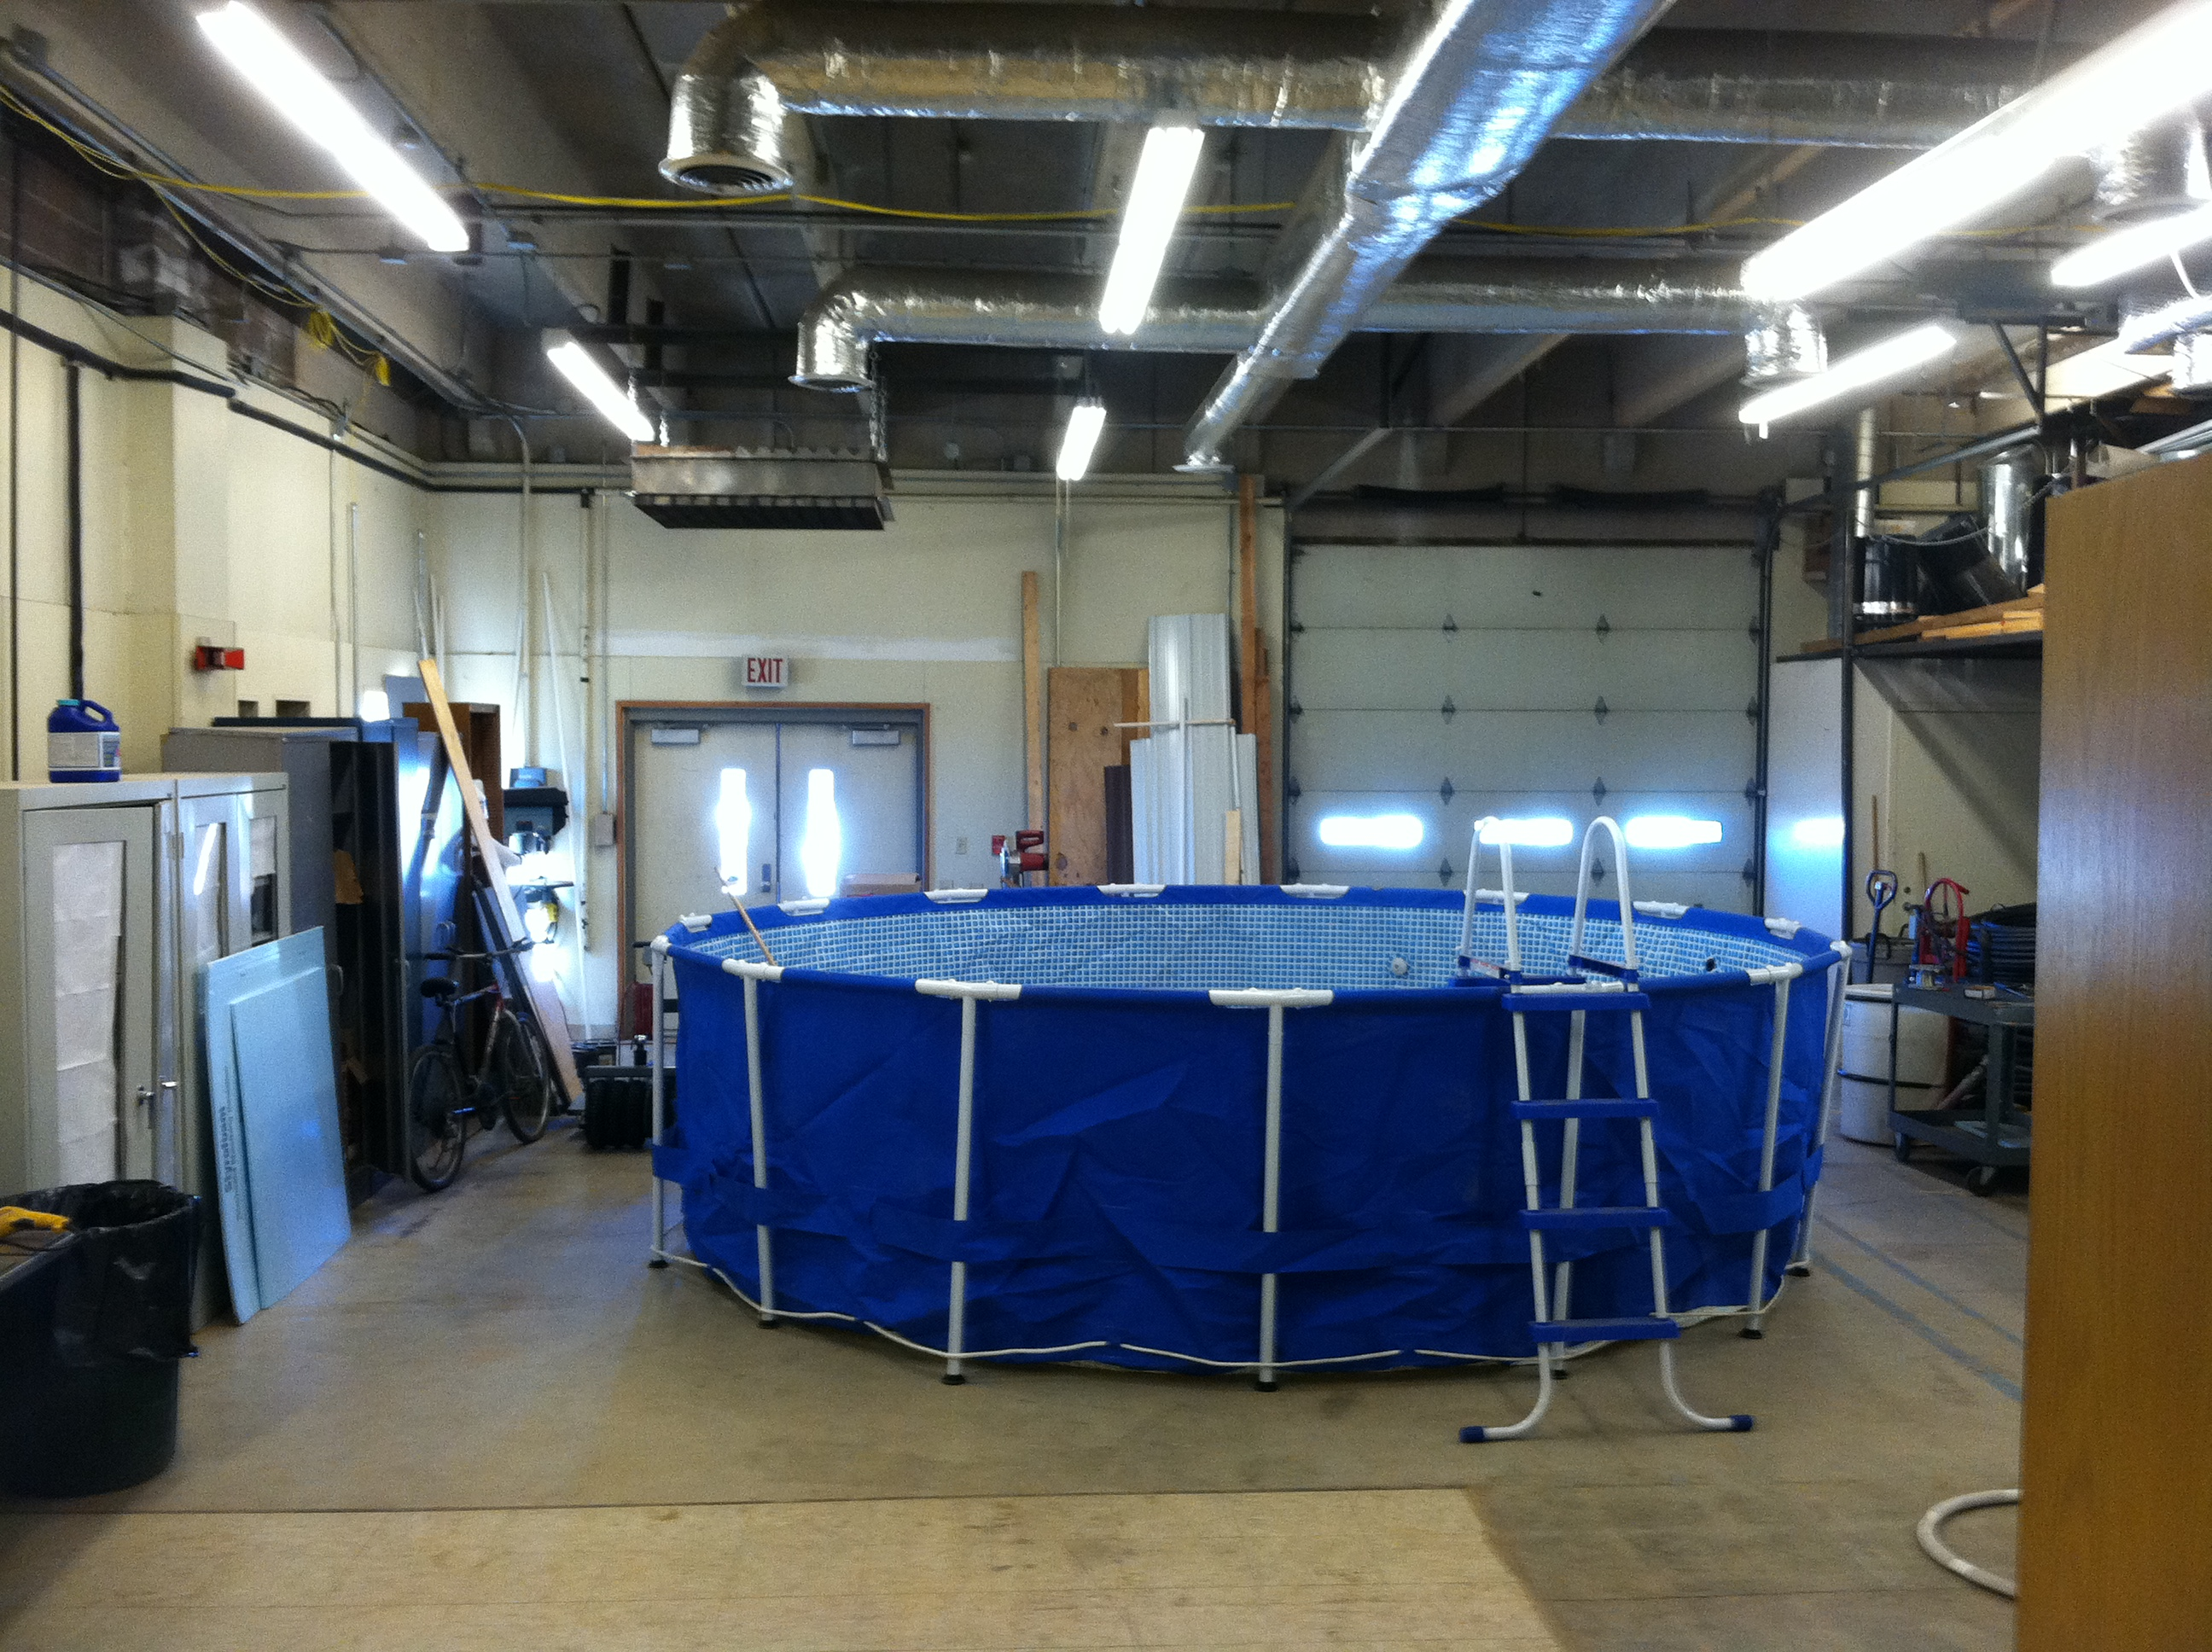
\includegraphics[width=0.8\textwidth]{Pool.jpg}
		\caption[Uninsulated indoor test pool]{Pool used for testing spiral-helical SWHE in laboratory facility}
		\label{fig:ExpMethod:HeatExtr:Apparatus:EmptyPool}
	\end{figure}

	\begin{figure}
		\centering
		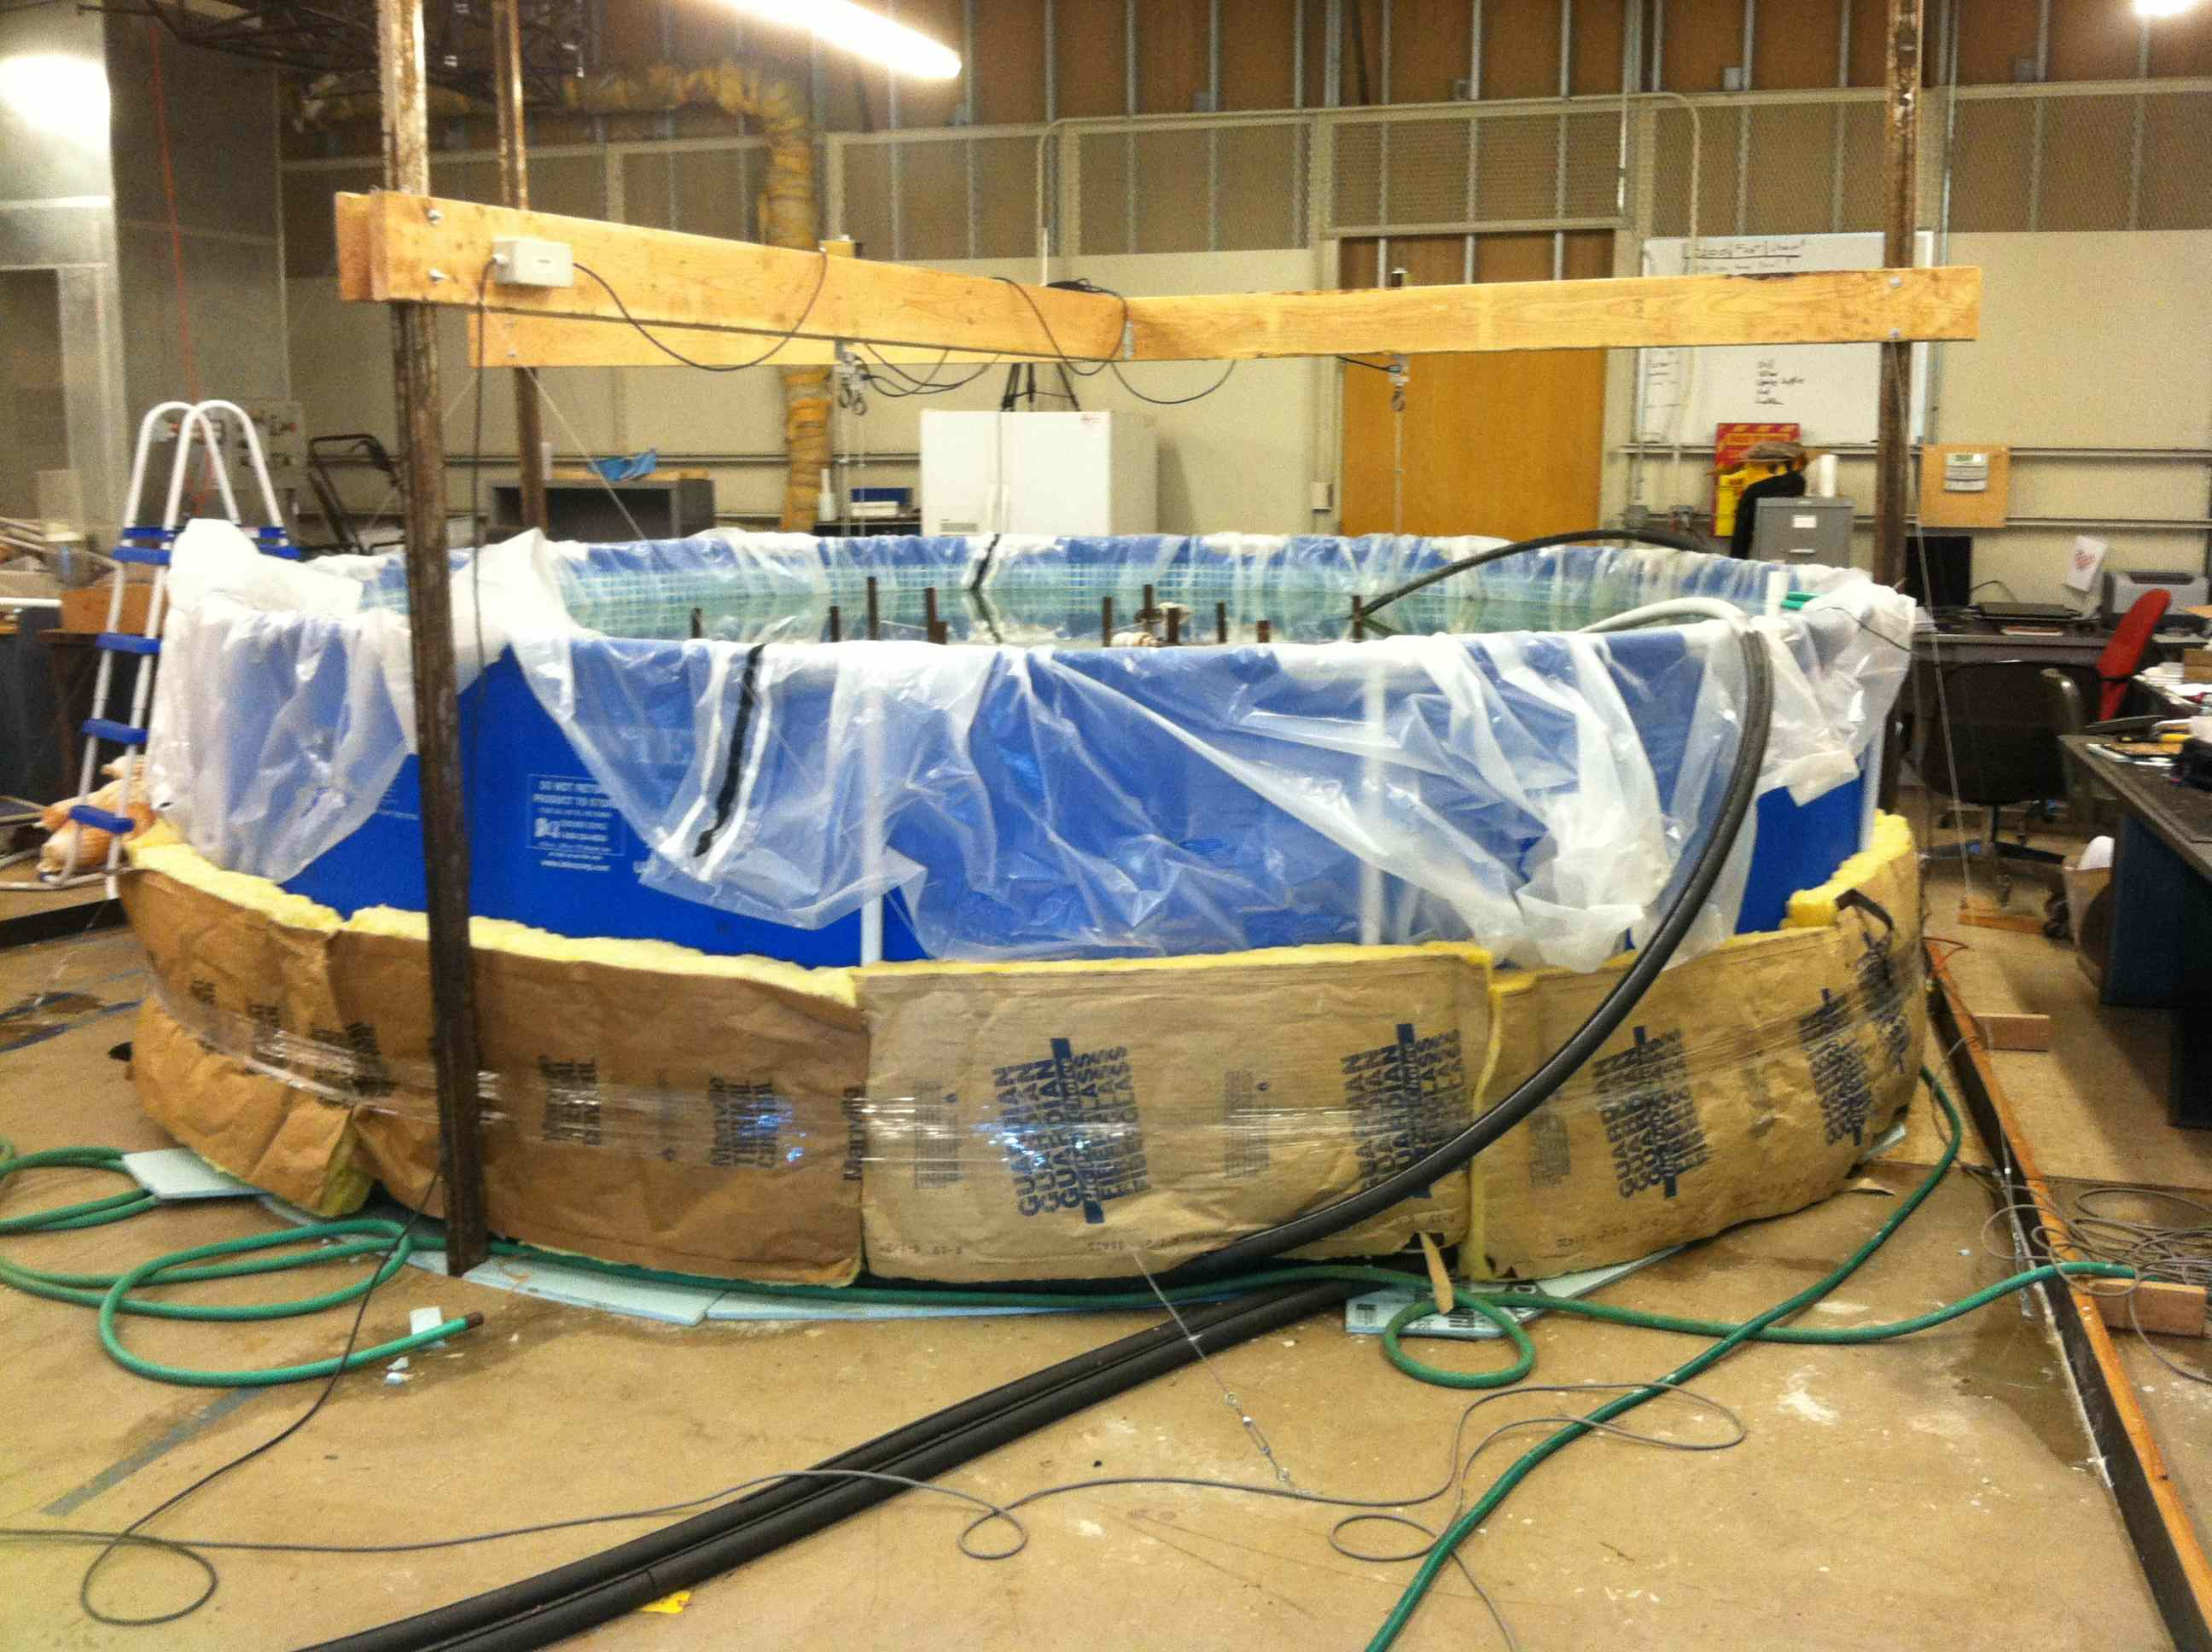
\includegraphics[width=0.8\textwidth]{Pool_Full.jpg}
		\caption[Indoor test pool during experiment]{Experimental setup used for indoor heat exchanger tests}
		\label{fig:ExpMethod:HeatExtr:Apparatus:FullPool}
	\end{figure}

	\begin{figure}
		\centering
		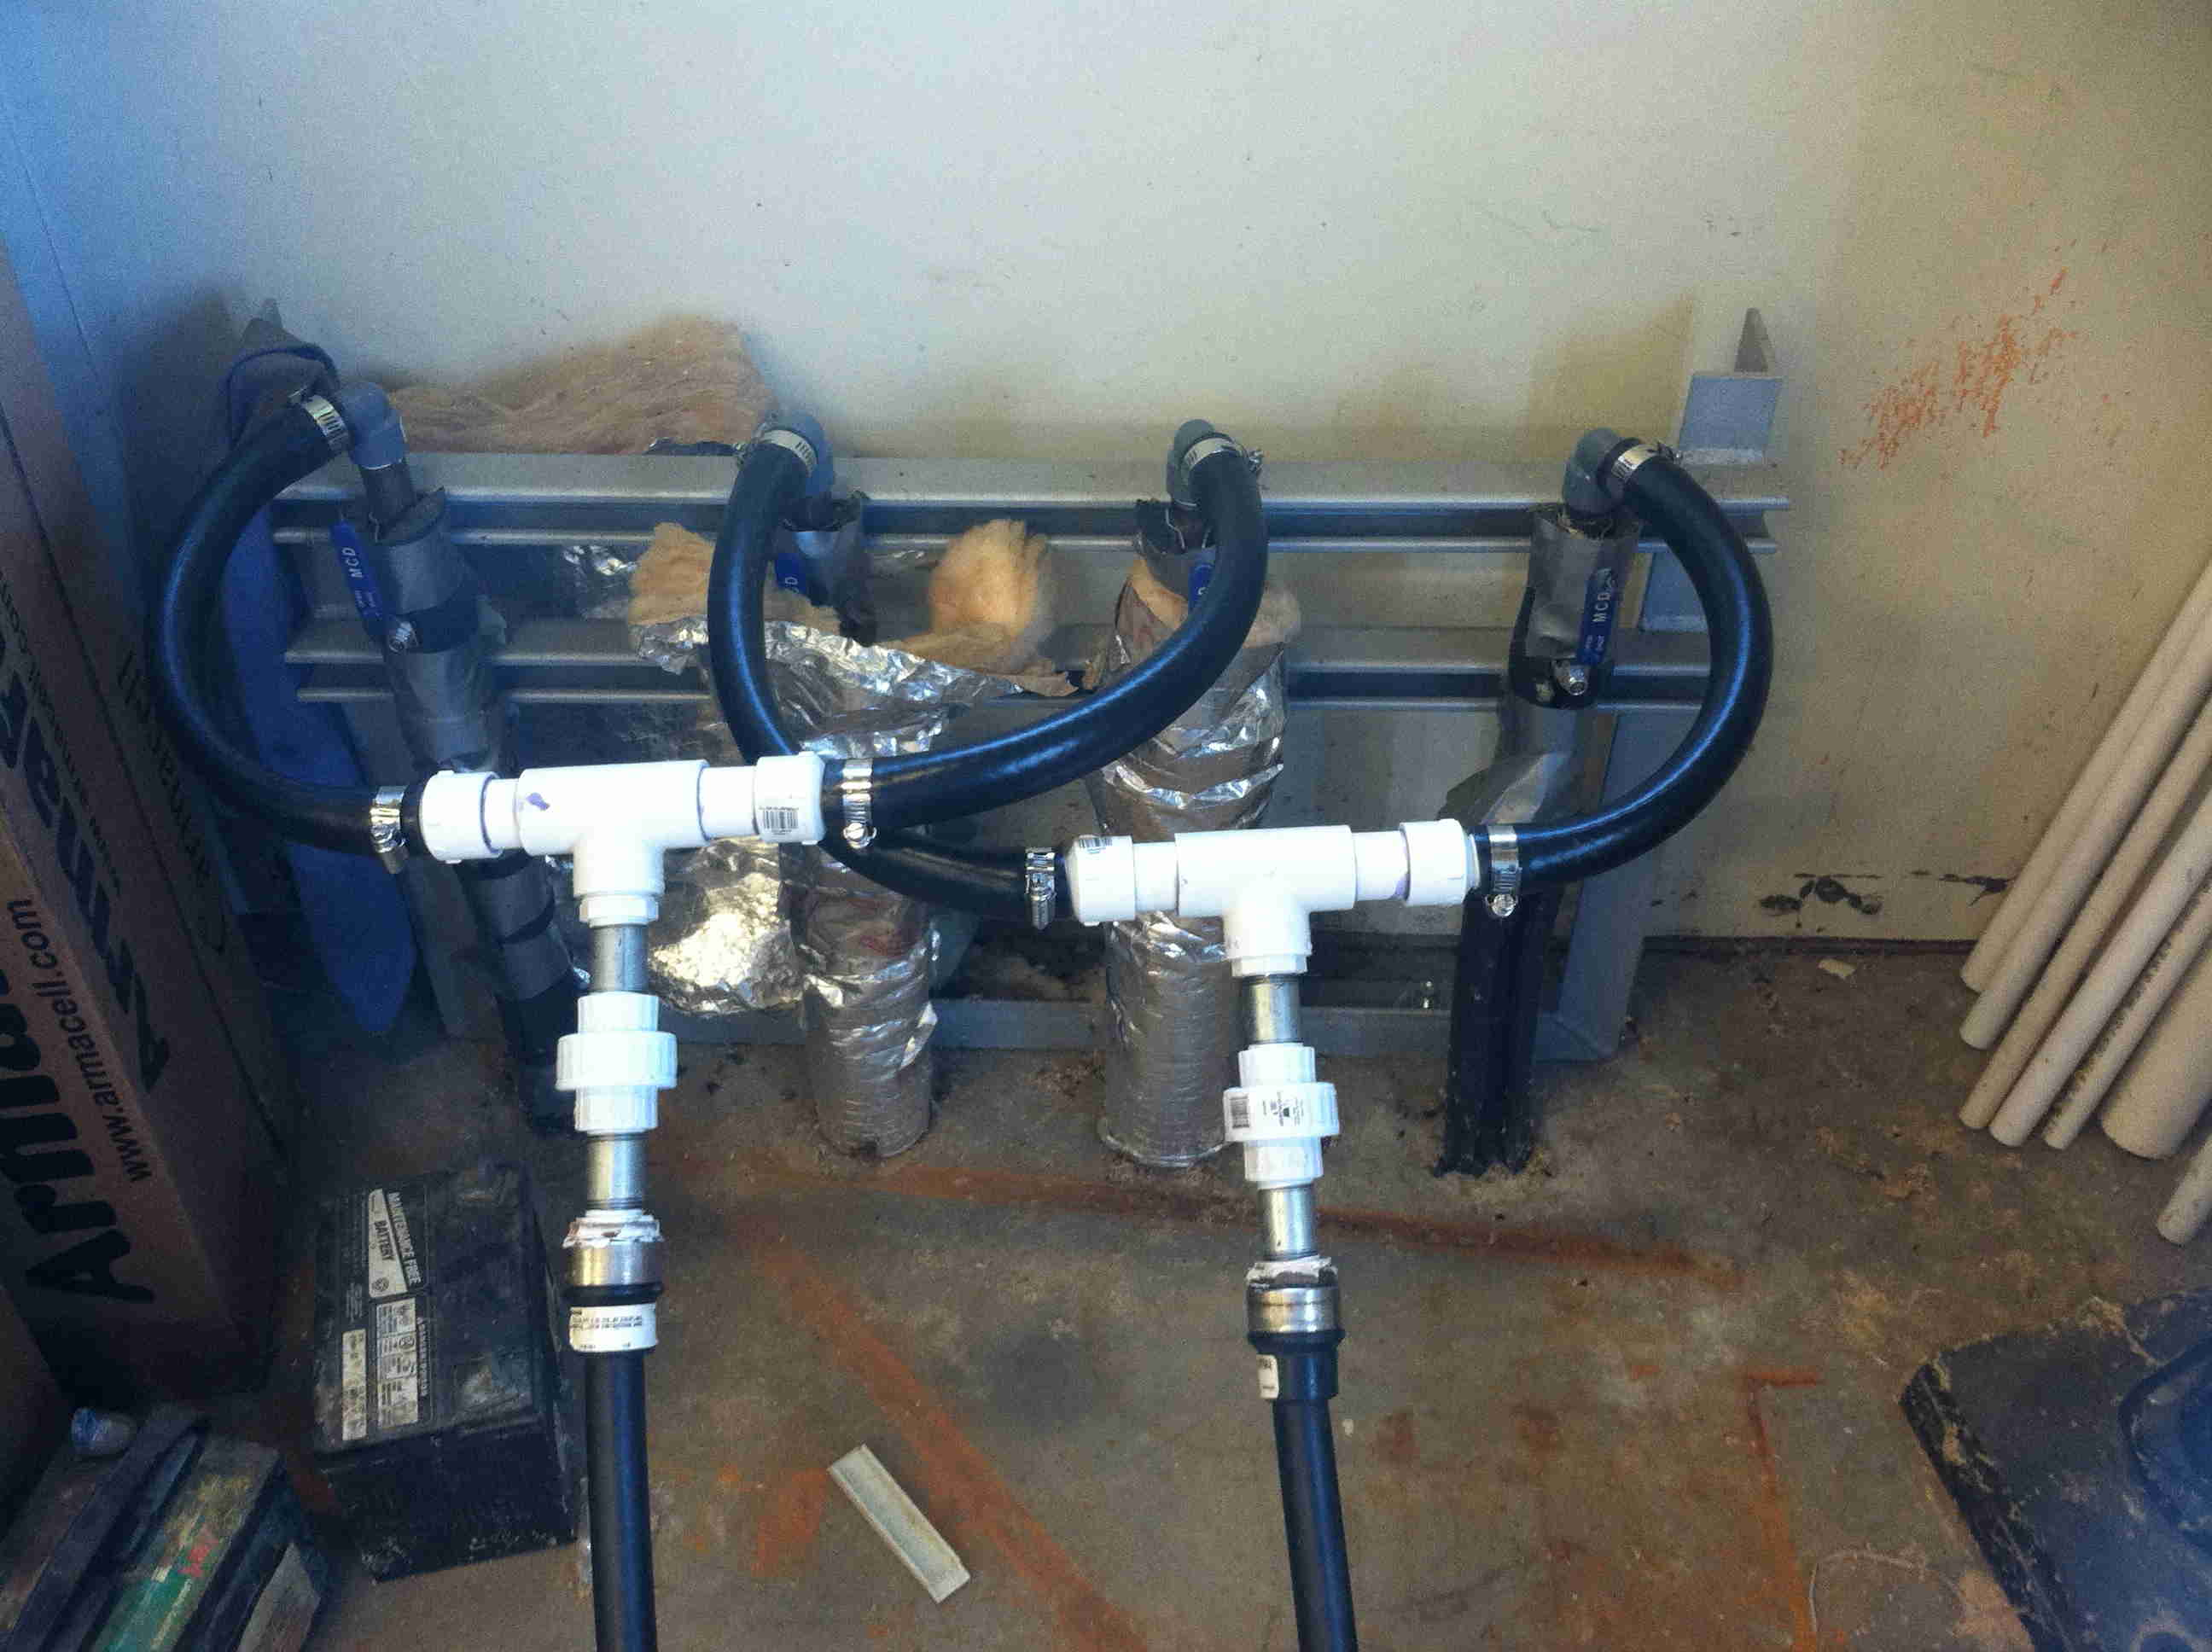
\includegraphics[width=0.8\textwidth]{GHX.jpg}
		\caption[Ground heat exchanger connections]{Ground heat exchanger connections where the water-water heat pump rejected/extracted excess heat energy}
		\label{fig:ExpMethod:HeatExtr:Apparatus:GHX}
	\end{figure}

Once the heat extraction experiment had been moved indoors, it was discovered that the submersible load cells had been damaged during the transport of the load cell frame from the pond to the laboratory facility. Due to this, new tension only load cells were purchased. These load cells have a capacity of 500 lb (227 kg) and can be seen in Figure \ref{fig:ExpMethod:HeatExtr:Apparatus:TensionLoadCell}. These load cells were less expensive than the original submersible load cells and ultimately would have been a better choice, due to the fragility of the submersible load cells. The SWHE and weighted SWHE support were then suspended from a support frame spanning the width of the pool. This support frame can be seen in Figure \ref{fig:ExpMethod:HeatExtr:Apparatus:WoodSupportFrame}. The tension only load cells were then used to measure the weight of the SWHE, along with the support frame, during the experiments. From this, the ice mass can be calculated. A schematic of the indoor pool, load cell frame, and support structure can be seen in Figure \ref{fig:ExpMethod:HeatExtr:Apparatus:ExtrExpPool}.

Pool water temperature measurements were taken in the pool at a distance of 4 ft.\ (1.2 m) away from the SWHE. Pool temperature was determined by averaging the temperature across the SWHE, as is shown in Equation \ref{eq:ExpMethod:HeatRej:Apparatus:PondTemp}.

	\begin{figure}
		\centering
		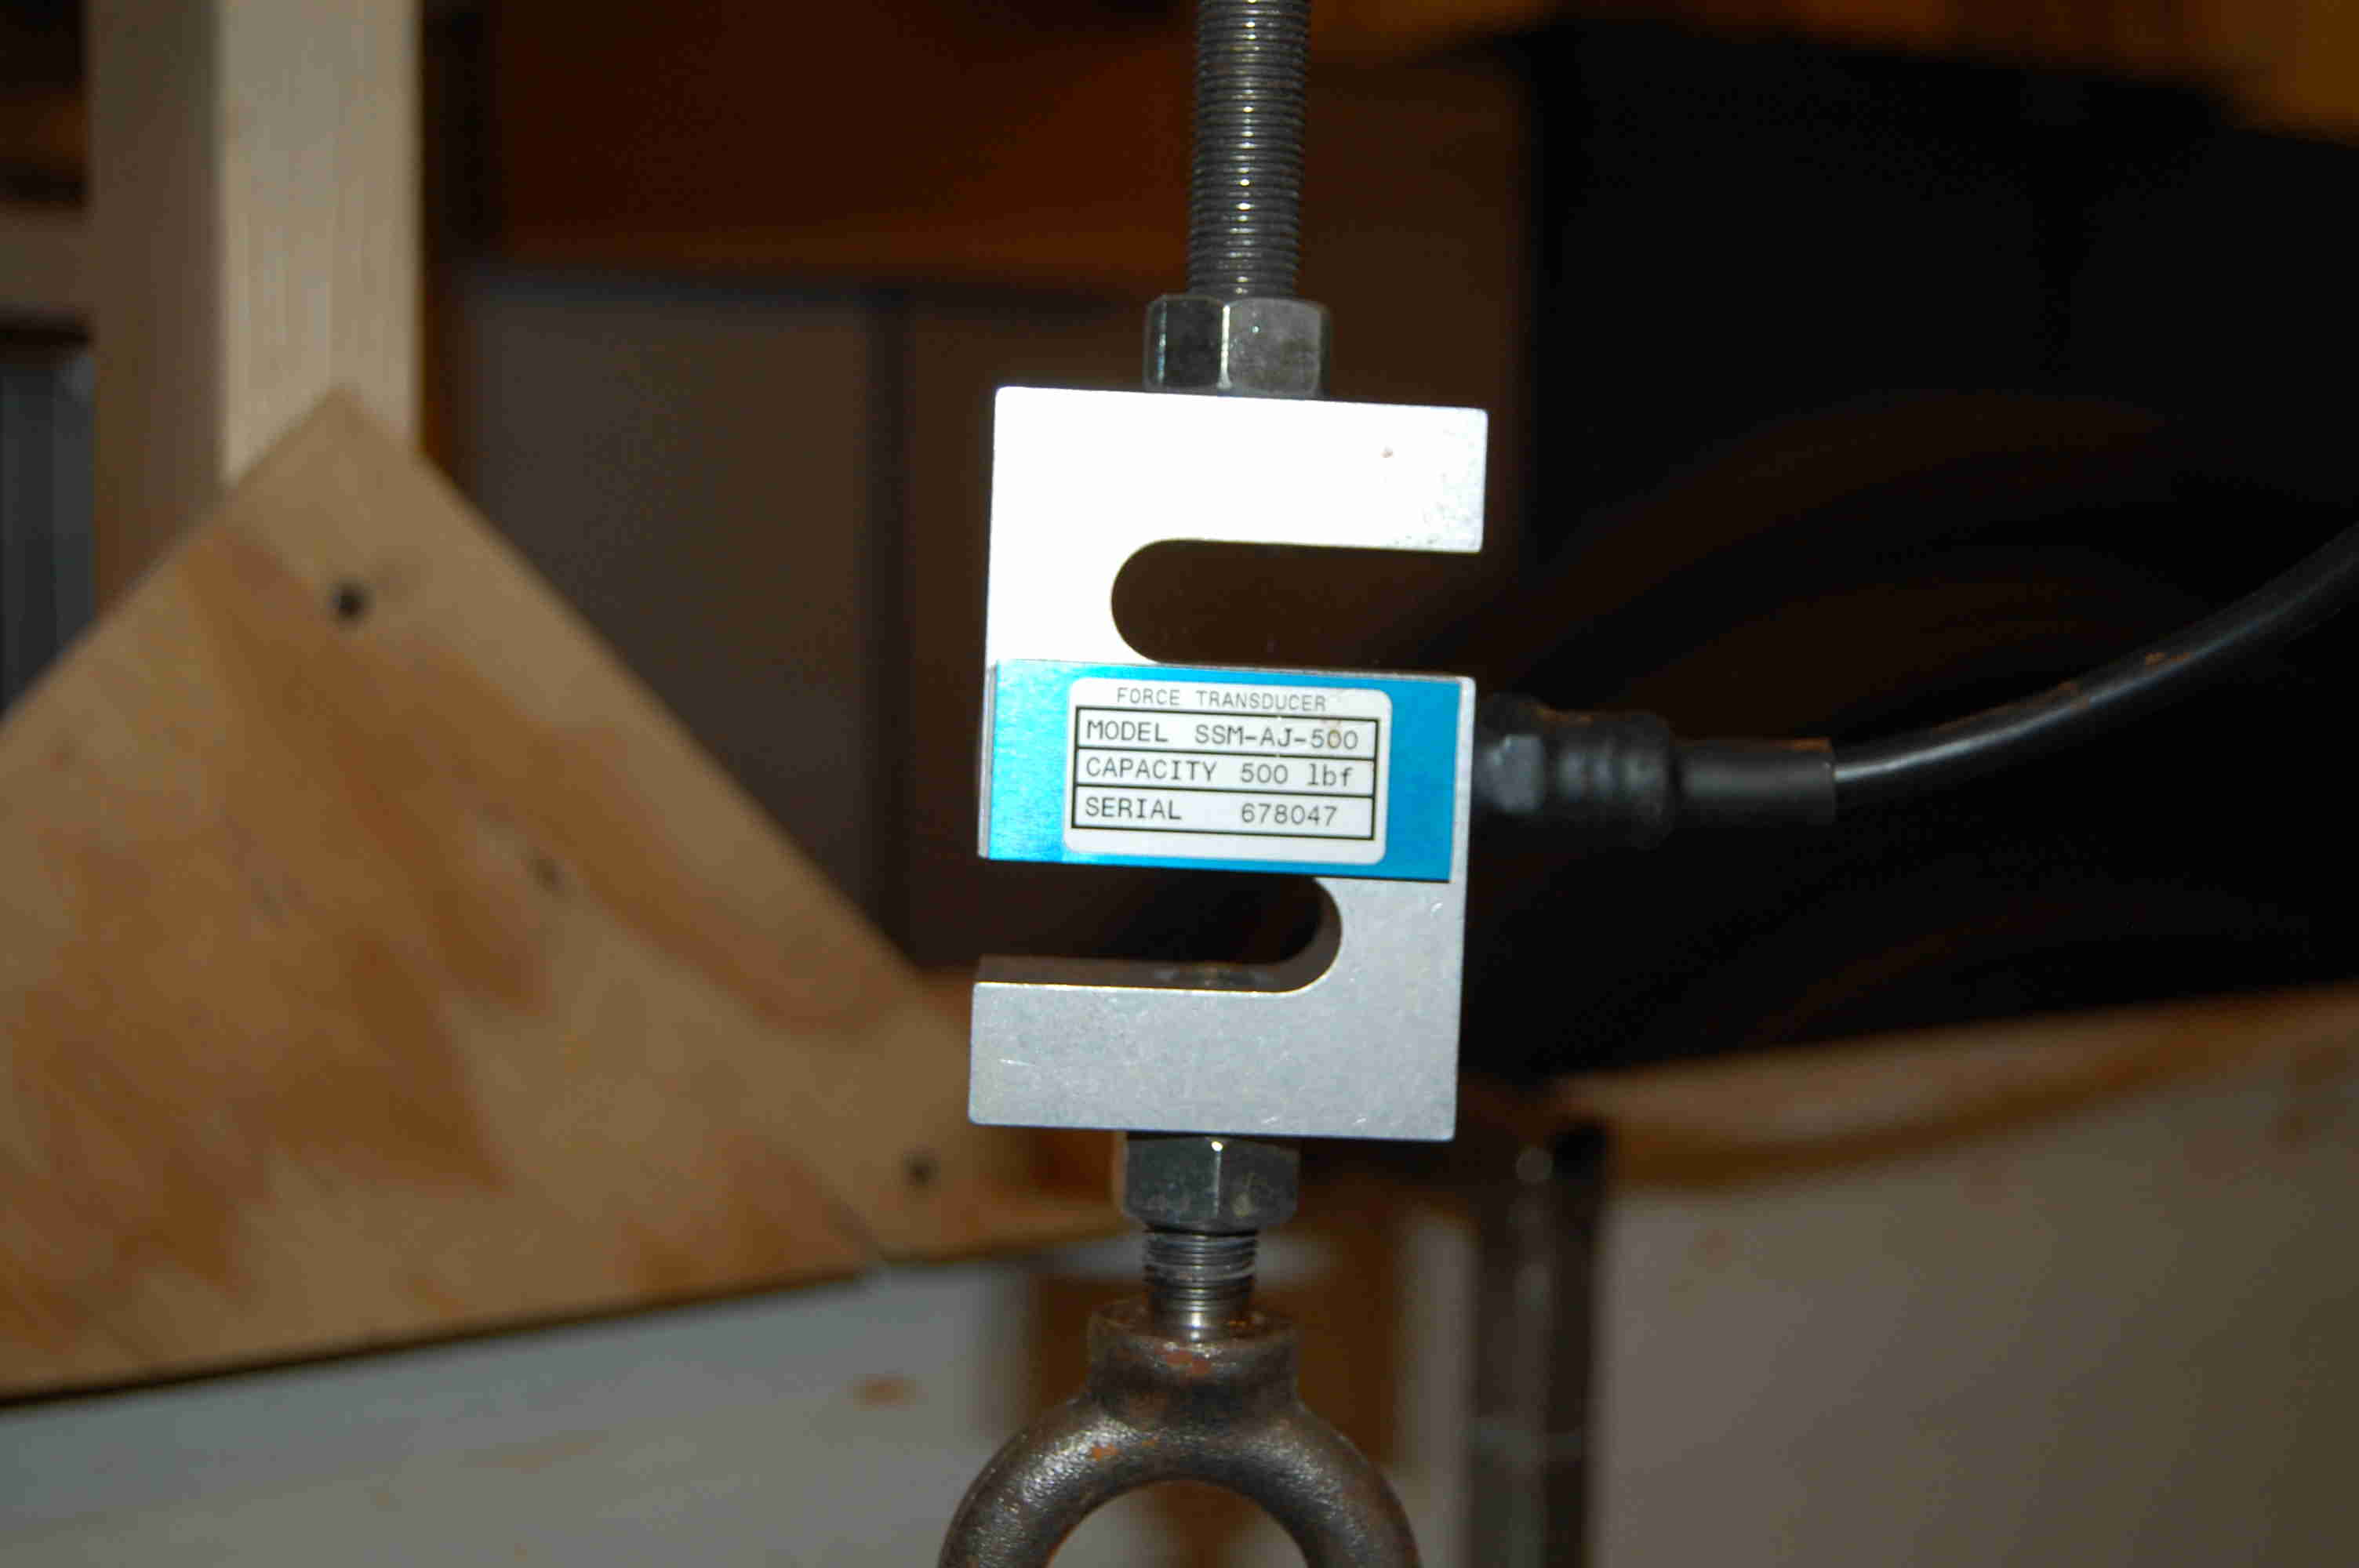
\includegraphics[width=0.8\textwidth]{TensionLoadCell.jpg}
		\caption[Tension only load cell]{Tension only load cell}
		\label{fig:ExpMethod:HeatExtr:Apparatus:TensionLoadCell}
	\end{figure}


	\begin{figure}
		\centering
		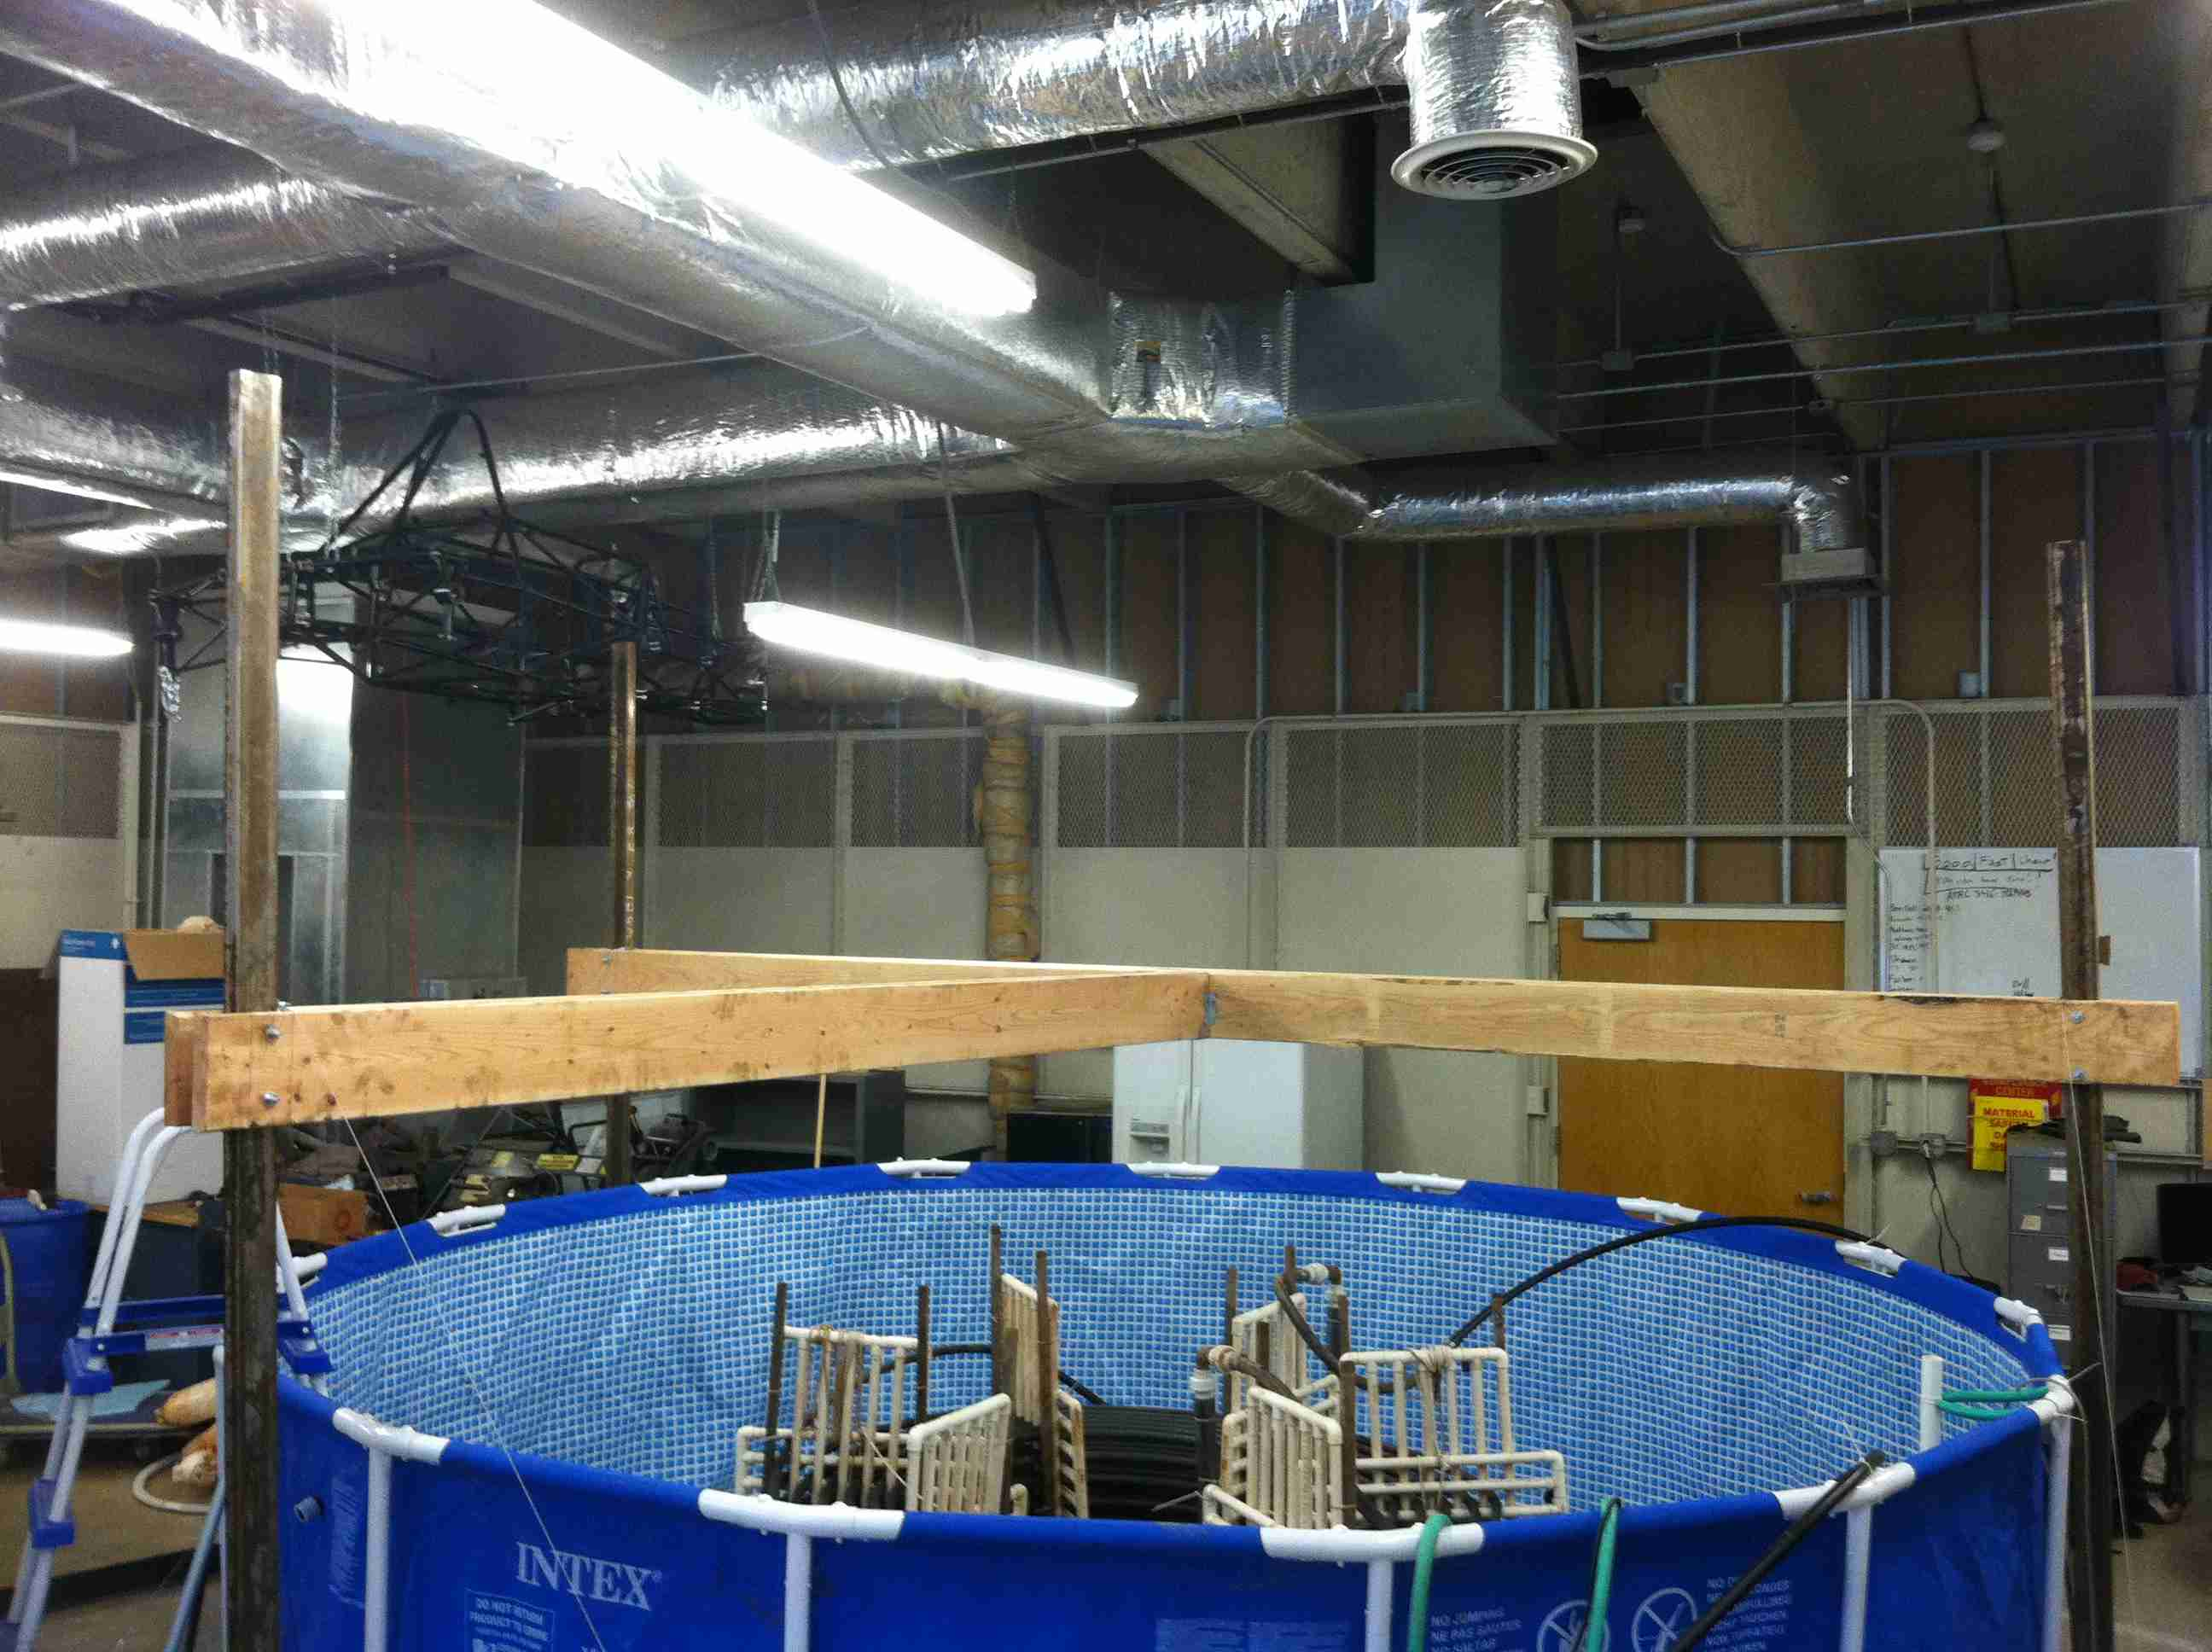
\includegraphics[width=0.8\textwidth]{WoodSupportFrame.jpg}
		\caption[Support frame used to support the weighted load cell frame]{Support frame used to support the weighted load cell frame}
		\label{fig:ExpMethod:HeatExtr:Apparatus:WoodSupportFrame}
	\end{figure}


	\begin{figure}
		\centering
		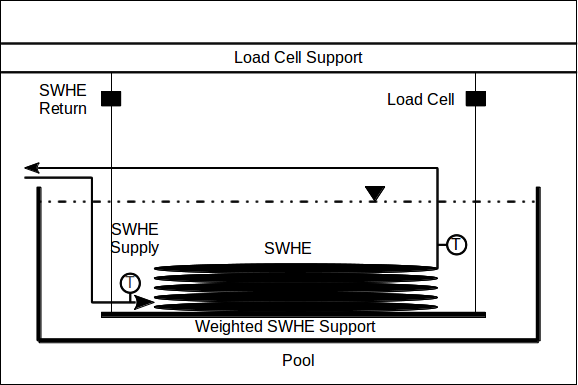
\includegraphics[width=0.8\textwidth]{SWHE_Ext_Pool.png}
		\caption[Schematic of heat extraction equipment in pool]{Schematic of heat extraction equipment in pool}
		\label{fig:ExpMethod:HeatExtr:Apparatus:ExtrExpPool}
	\end{figure}

	\subsection{Methodology}
	\label{subsec:ExpMethod:HeatExtr:Method}

Because the heat pumps we used for heat extraction were not variable speed machines, we were not able to vary heat transfer rates as was the case for the heat rejection tests. For these tests, the heat pumps were turned on and run for extended periods of time.

As was the case with heat the rejection tests, coil entering and exiting fluid temperatures were measured as was circulating fluid flow rate through a calibrated turbine flow meter. The heat pump entering and exiting fluid temperatures were also measured; however, the temperatures were not directly used to determine heat exchanger performance.

Total coil frame weight was also measured, which is the combined weight of the coil support frame and the coil. From this, the buoyancy force generated from the ice formation could then be estimated by subtracting the current weight from the weight at the beginning of the test.

\section{Instrumentation}
\label{sec:ExpMethod:Instr}

	\subsection{Temperature Measurement}
	\label{subsec:ExpMethod:Instr:Temp}

Two types of temperature sensors were used to measure temperature. The first temperature sensor was an in-pipe thermistor which was used to measure the circulating fluid temperature at the SWHE inlet and outlet. A photo of the in-pipe thermistor can be seen in Figure \ref{fig:ExpMethod:Instr:Temp:Thermistor}. The thermistors were purchased from Omega Engineering and have a model number of: ON-410-PP.

\begin{figure}
	\centering
	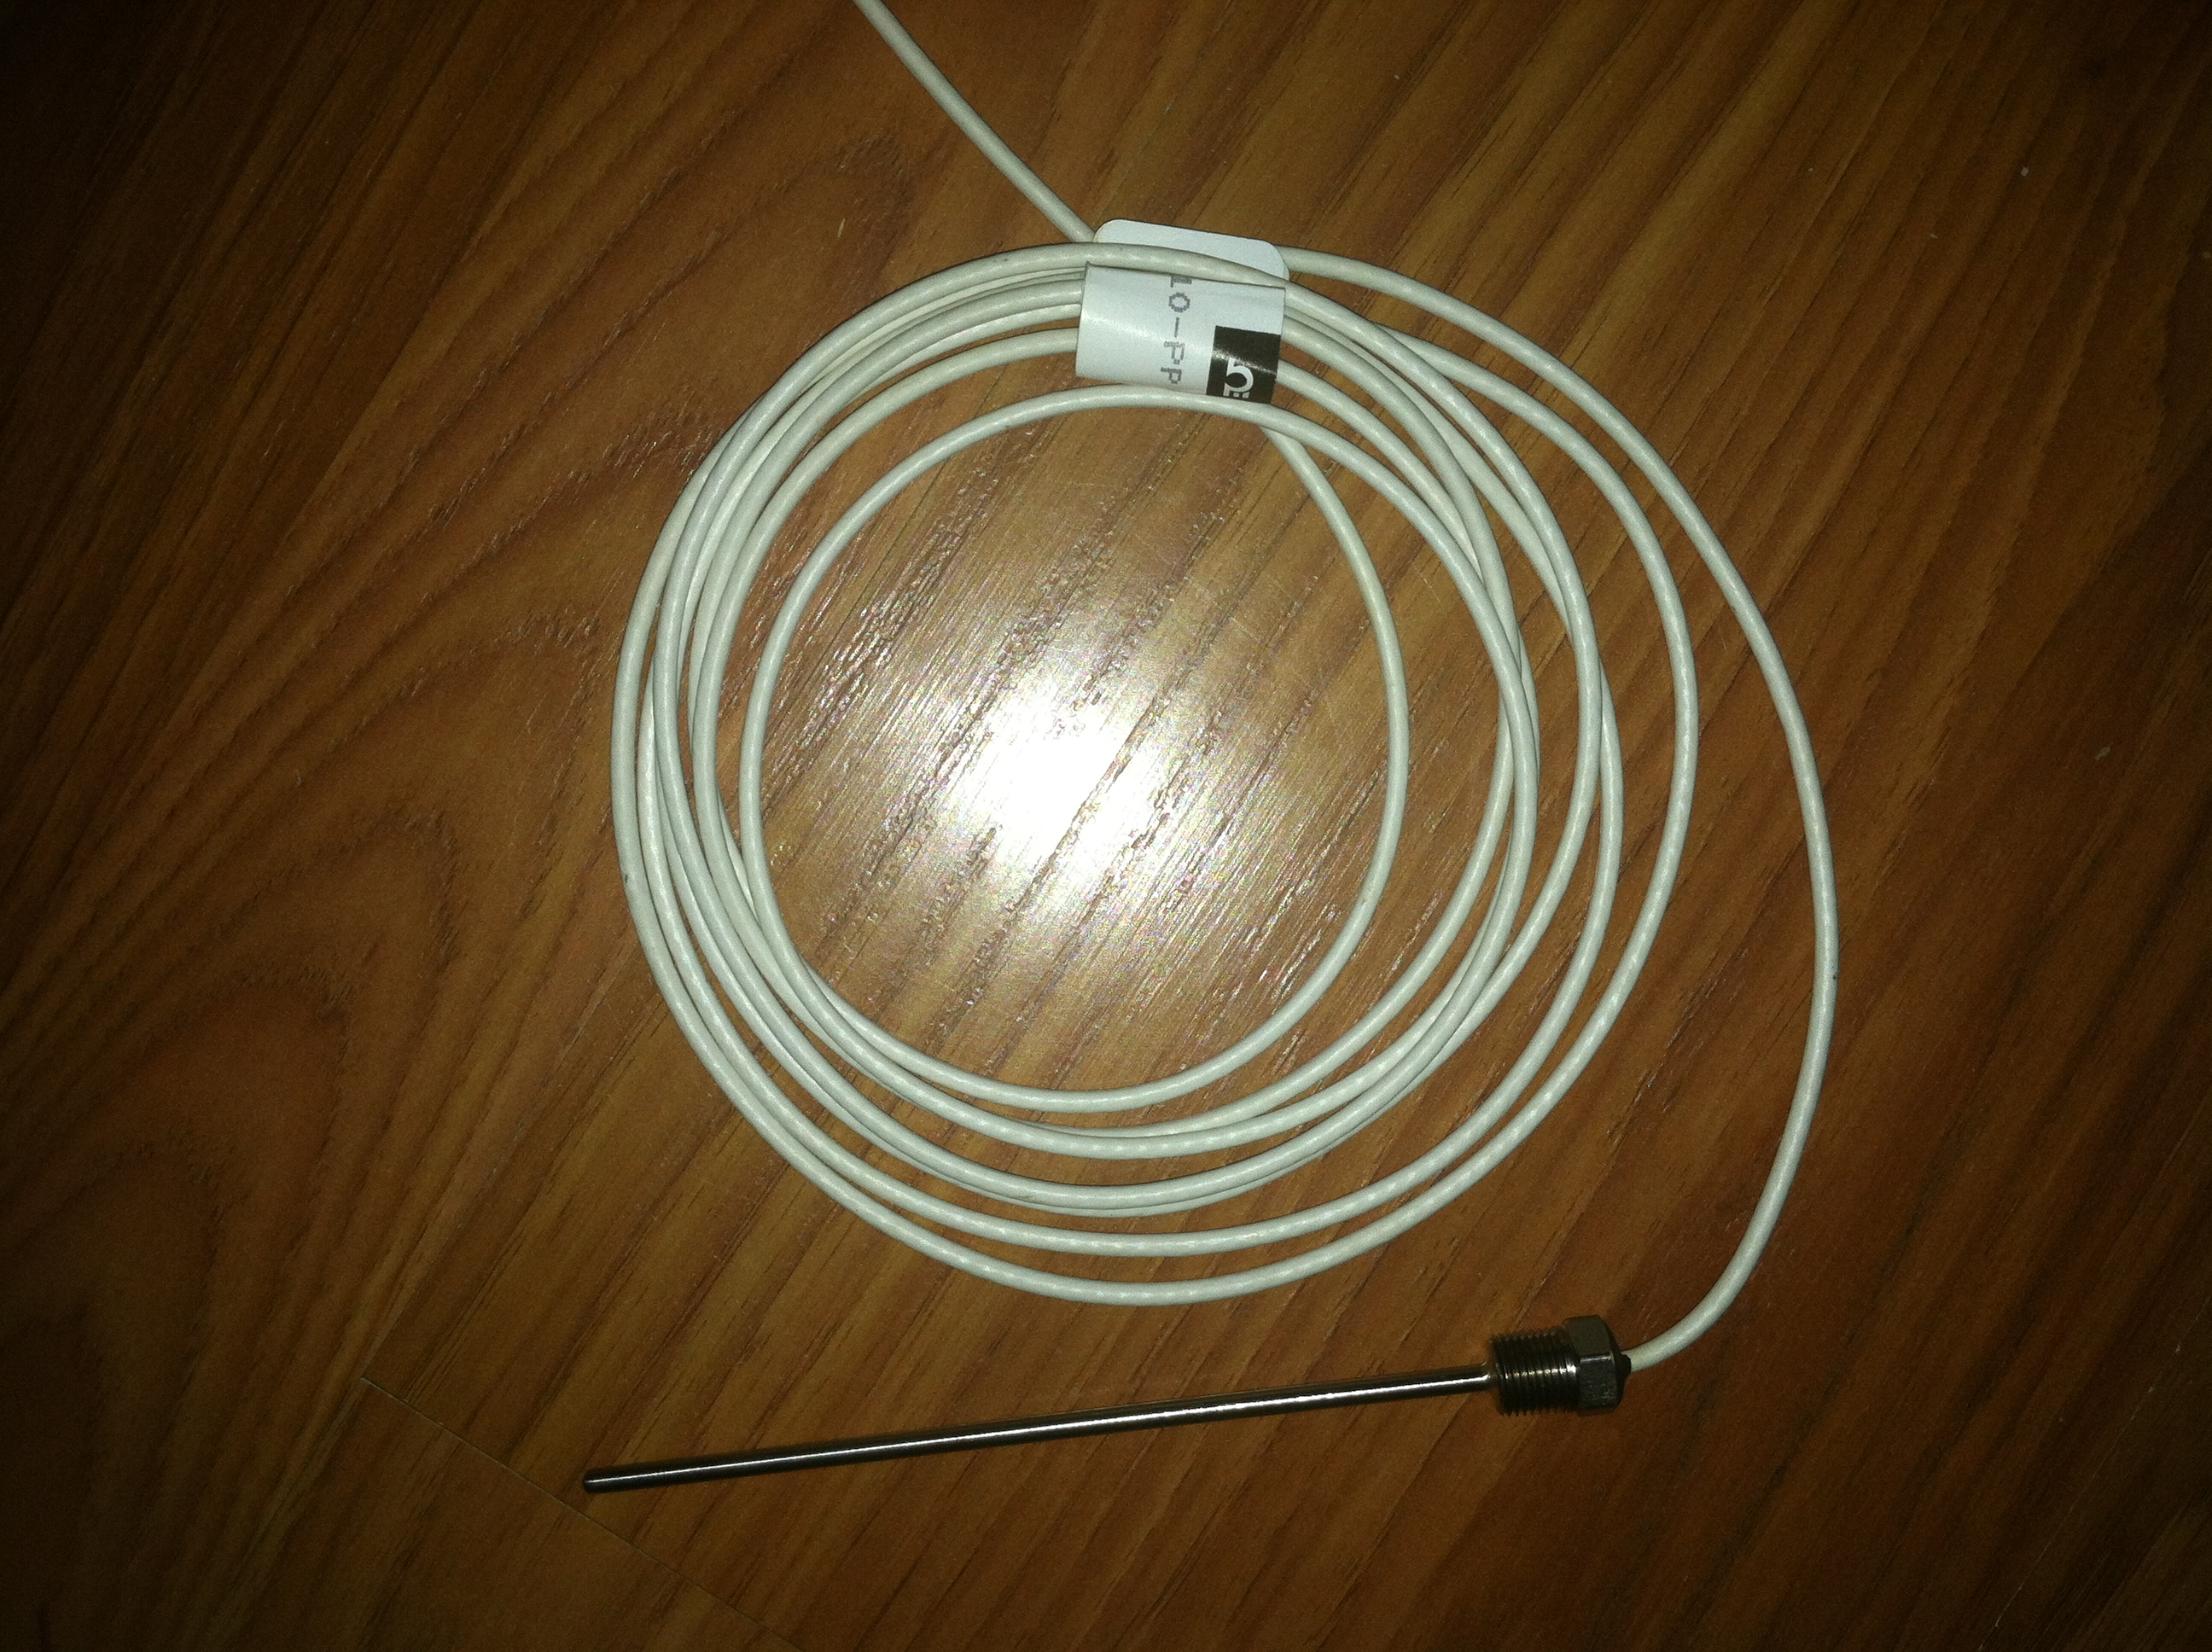
\includegraphics[width=0.8\textwidth]{Thermistor.jpeg}
	\caption[In-pipe thermistor]{In-pipe thermistor used to measure circulating fluid inlet and outlet temperature}
	\label{fig:ExpMethod:Instr:Temp:Thermistor}
\end{figure}

The second type of temperature sensor is a thermistor which which was soldered to 22 ga.\ (0.644 mm) instrumentation wire. These thermistors were used to measure the surface water temperatures in the pond and pool during experiments. A photo of one of these thermistors can be seen in Figure \ref{fig:ExpMethod:Instr:Temp:SmallThermistor}. The thermistors were purchased from Jameco Electronics and have a model number of: 207037.

\begin{figure}
	\centering
	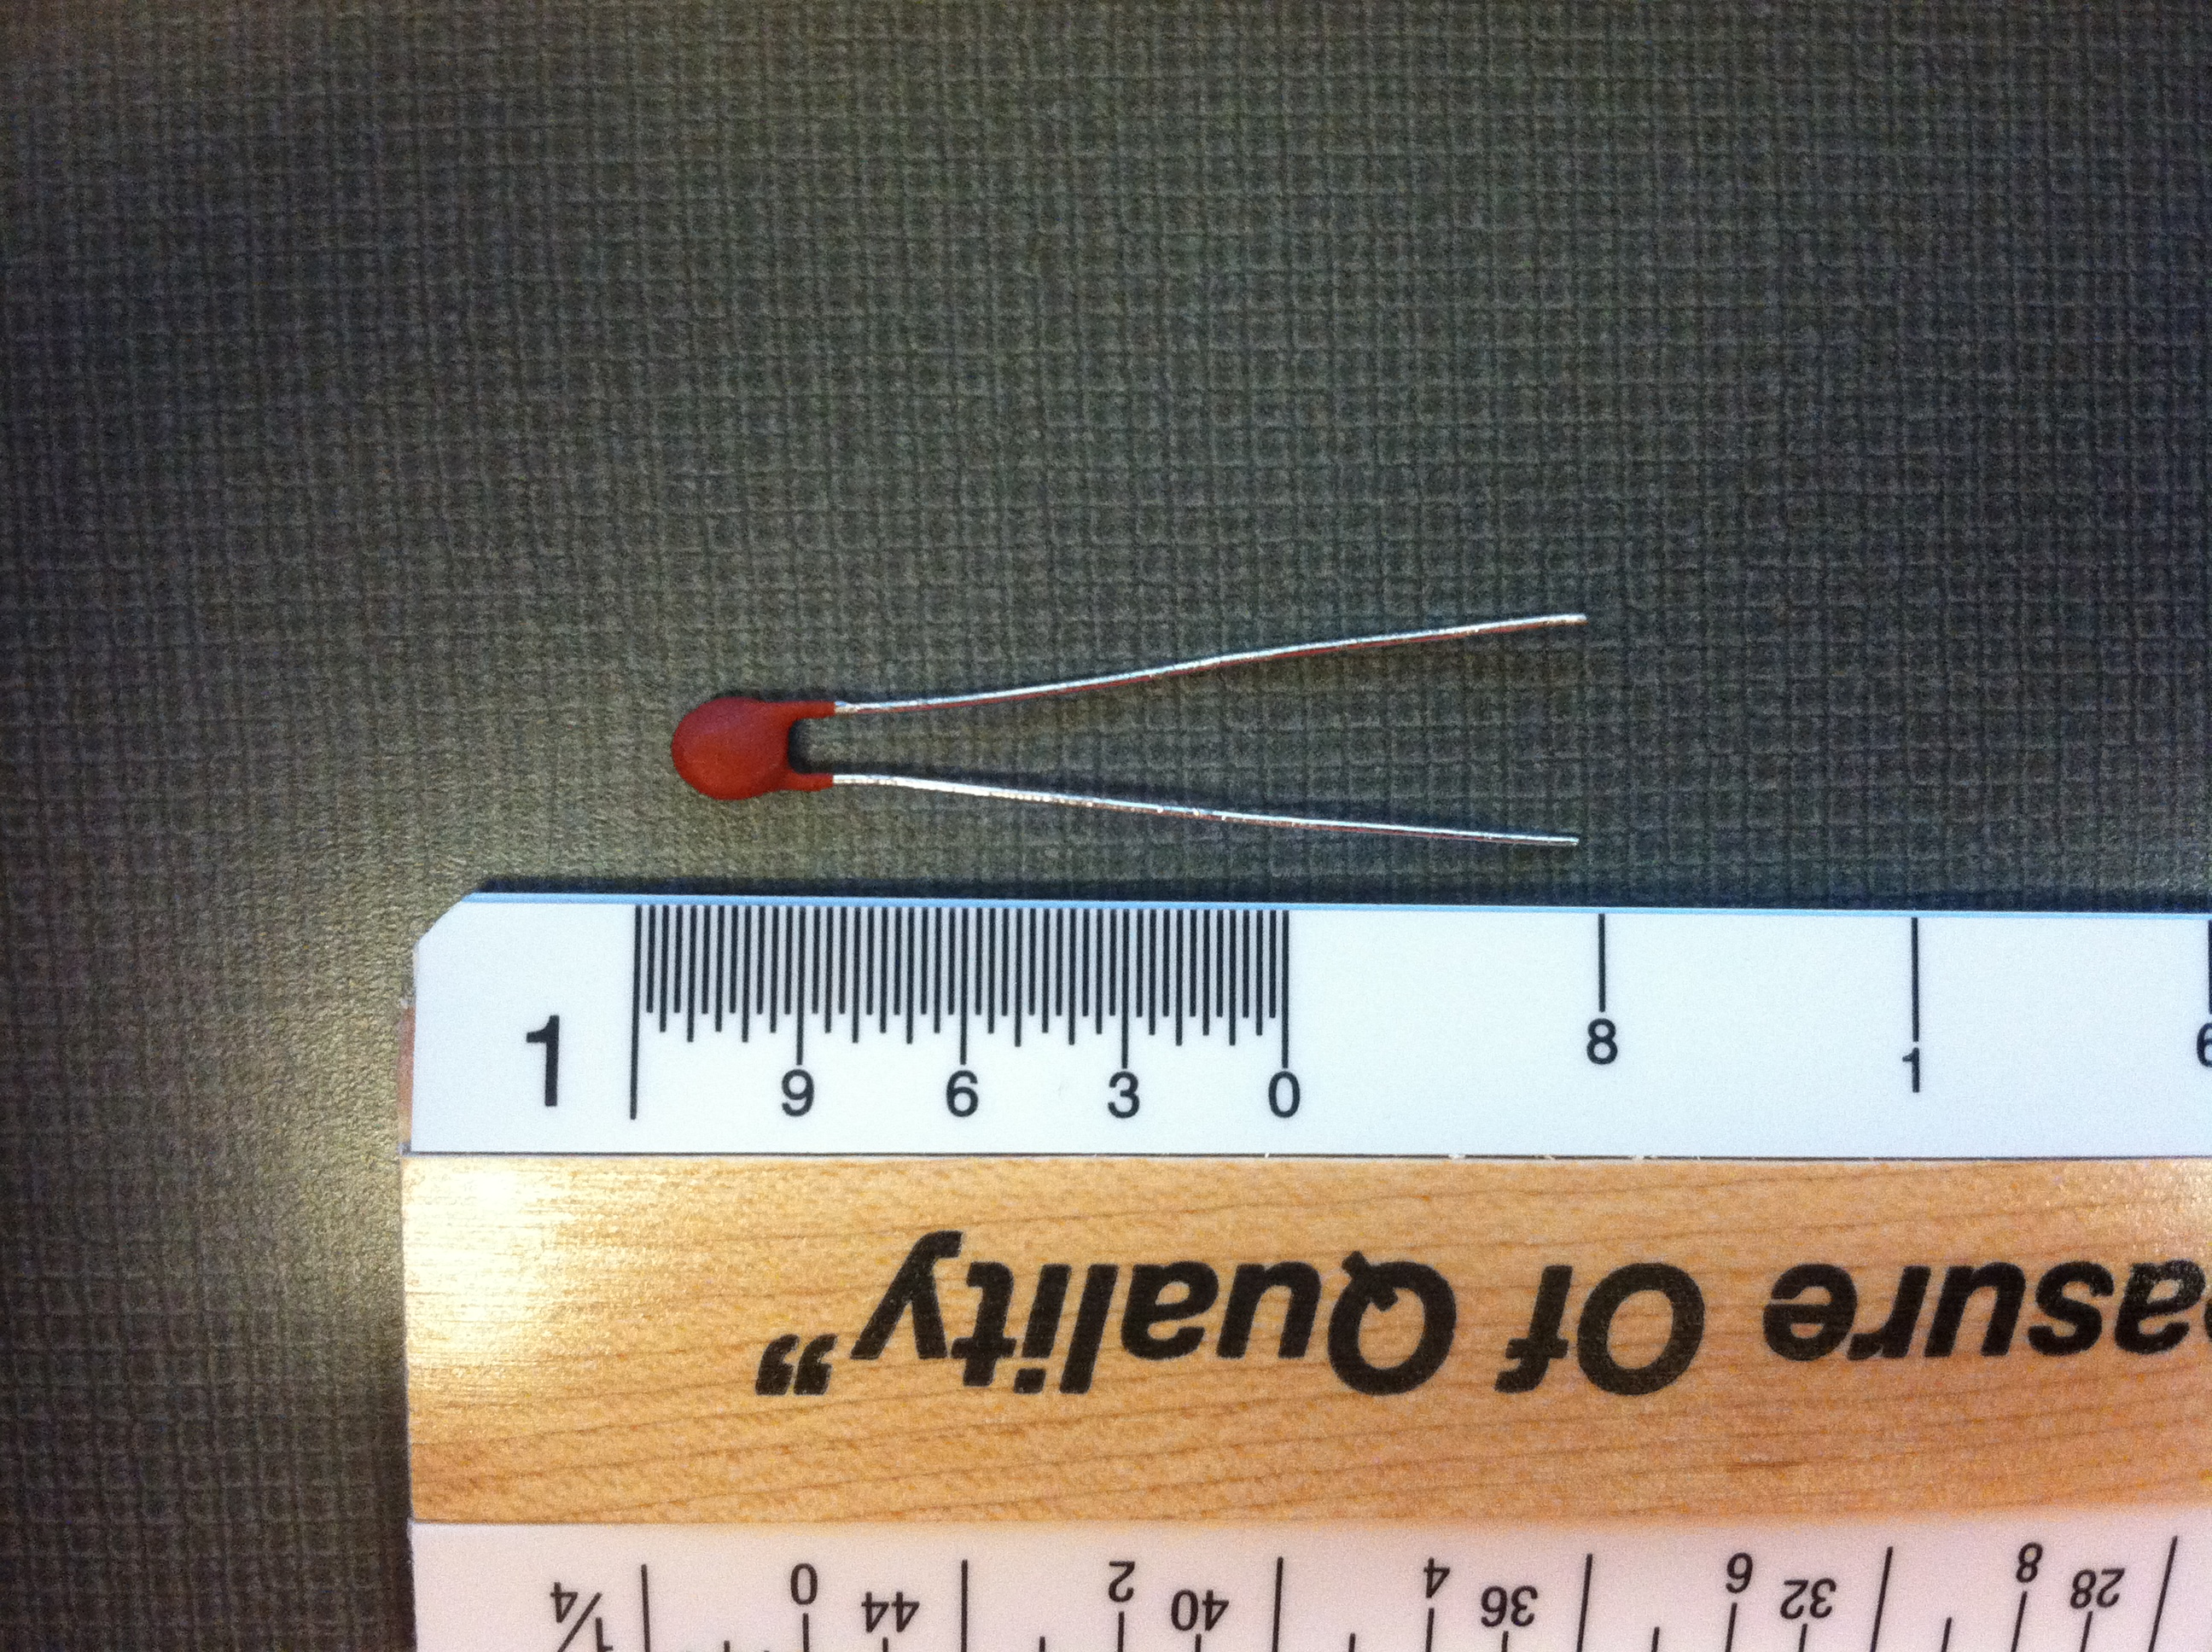
\includegraphics[width=0.8\textwidth]{SmallThermistor.jpg}
	\caption[Small thermistor]{Thermistor for surface water temperature measurement}
	\label{fig:ExpMethod:Instr:Temp:SmallThermistor}
\end{figure}

After the smaller thermistor was soldered to the 22 ga.\ (0.644 mm) instrumentation wire, it was coated in marine epoxy up to the tip to prevent the lead wires from touching. This epoxy also seals the soldered connections preventing surface water from causing a short in the electrical circuit. A photo of an epoxied themistor can be see in Figure \ref{fig:ExpMethod:Instr:Temp:SmallThemistor:Epoxy}.

\begin{figure}
	\centering
	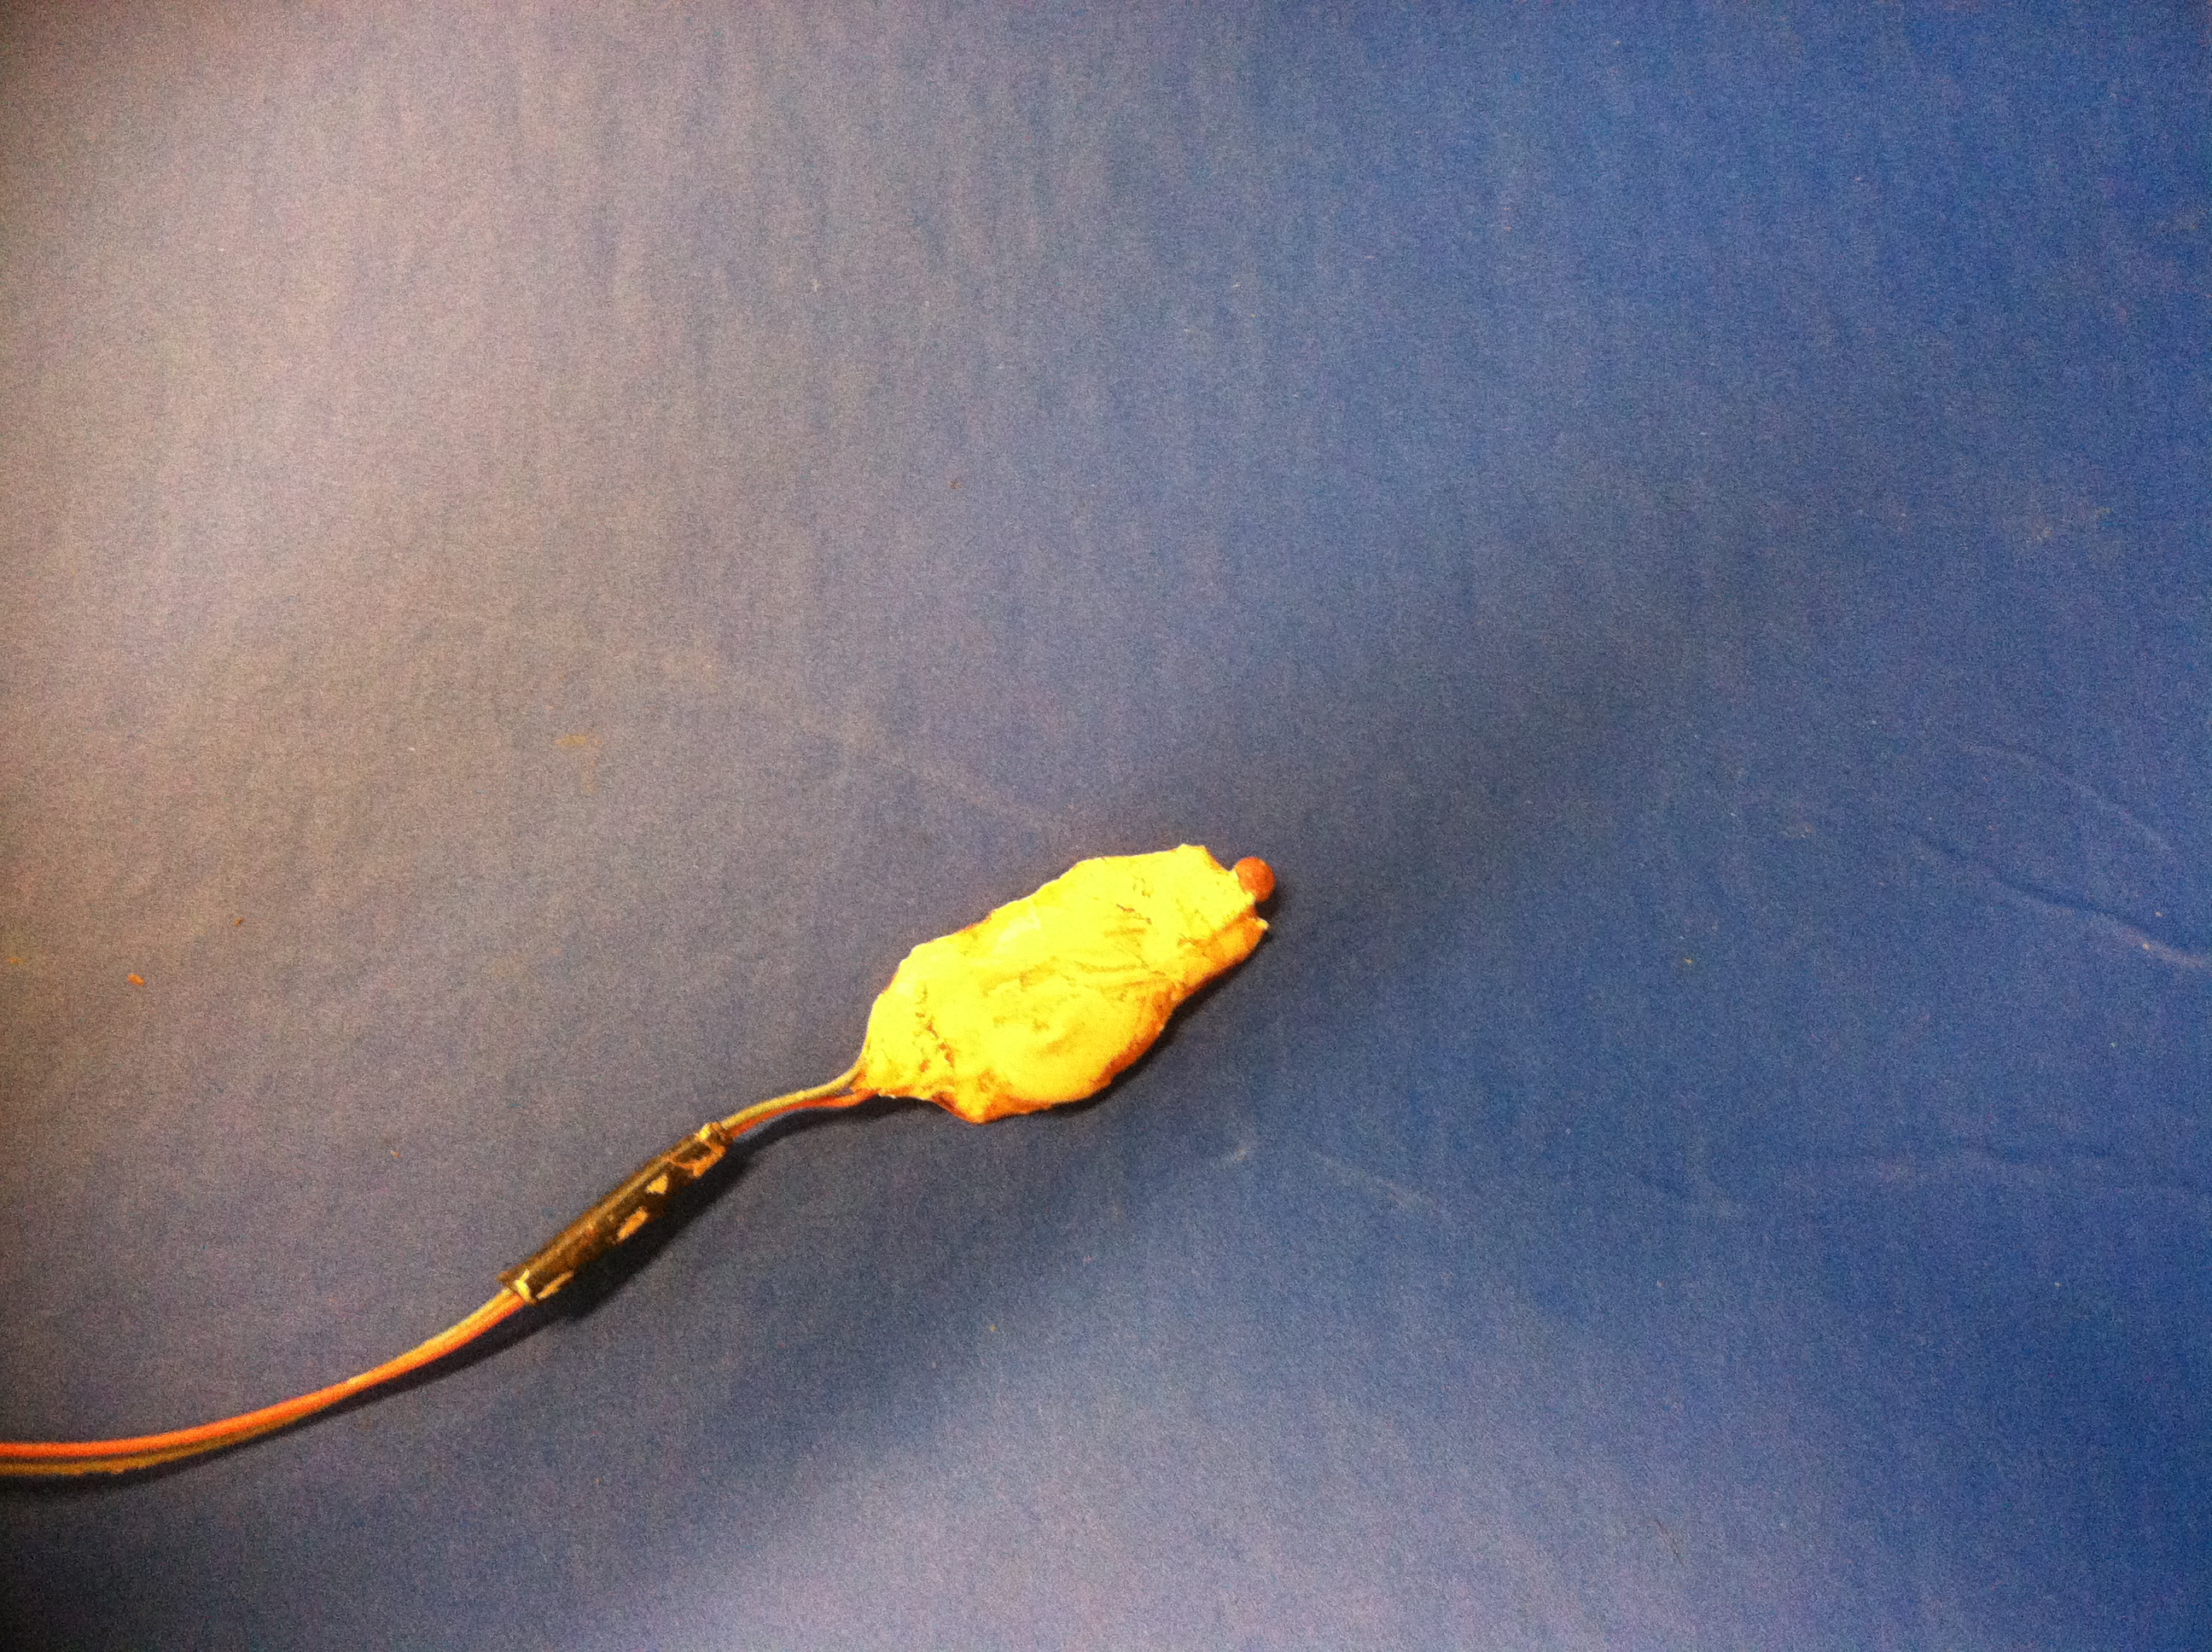
\includegraphics[width=0.8\textwidth]{SmallThermistor_Epoxy.jpg}
	\caption[Epoxy coated thermistor]{Themistor coated in epoxy up to the tip for surface water temperature measurement}
	\label{fig:ExpMethod:Instr:Temp:SmallThemistor:Epoxy}
\end{figure}

	\subsection{Temperature Measurement Calibration}
	\label{subsec:ExpMethod:Instr:TempCal}

The thermistors shown in Figure \ref{fig:ExpMethod:Instr:Temp:Thermistor} were also soldered to 22 ga.\ (0.644 mm) instrumentation wire. This was done so instrumentation wires could be run from the SHWE, which was submerged in the pond, to the data logger which was situated in the trailer several hundred feet away. Because of the instrumentation wire being added to the circuit, as well as the inherent uncertainty in the thermistor resistance, the thermistors needed to be calibrated with the leads attached so the temperatures could be accurately determined. Because thermistor resistance varies with temperature, the resistance was what was necessary to record in order to determine the temperature measurement.

To perform the calibration, the thermistors were placed in a calibration water bath, as is shown in Figure \ref{fig:ExpMethod:Instr:TempCal:CalBath}. This water bath was set at a given set point, then allowed to run to a steady state temperature. Once the bath temperature was constant, the resistance was measured every 5 seconds for 5 minutes. The average value of these measurements was then taken as the thermistor resistance at that given temperature. Bath temperature was determined from a glass spirit filled thermometer which was calibrated to 0.09$^\circ$F (0.05$^\circ$C). This thermometer is also visible in Figure \ref{fig:ExpMethod:Instr:TempCal:CalBath}. The thermometer was manufactured by ERTCO.

\begin{figure}
	\centering
	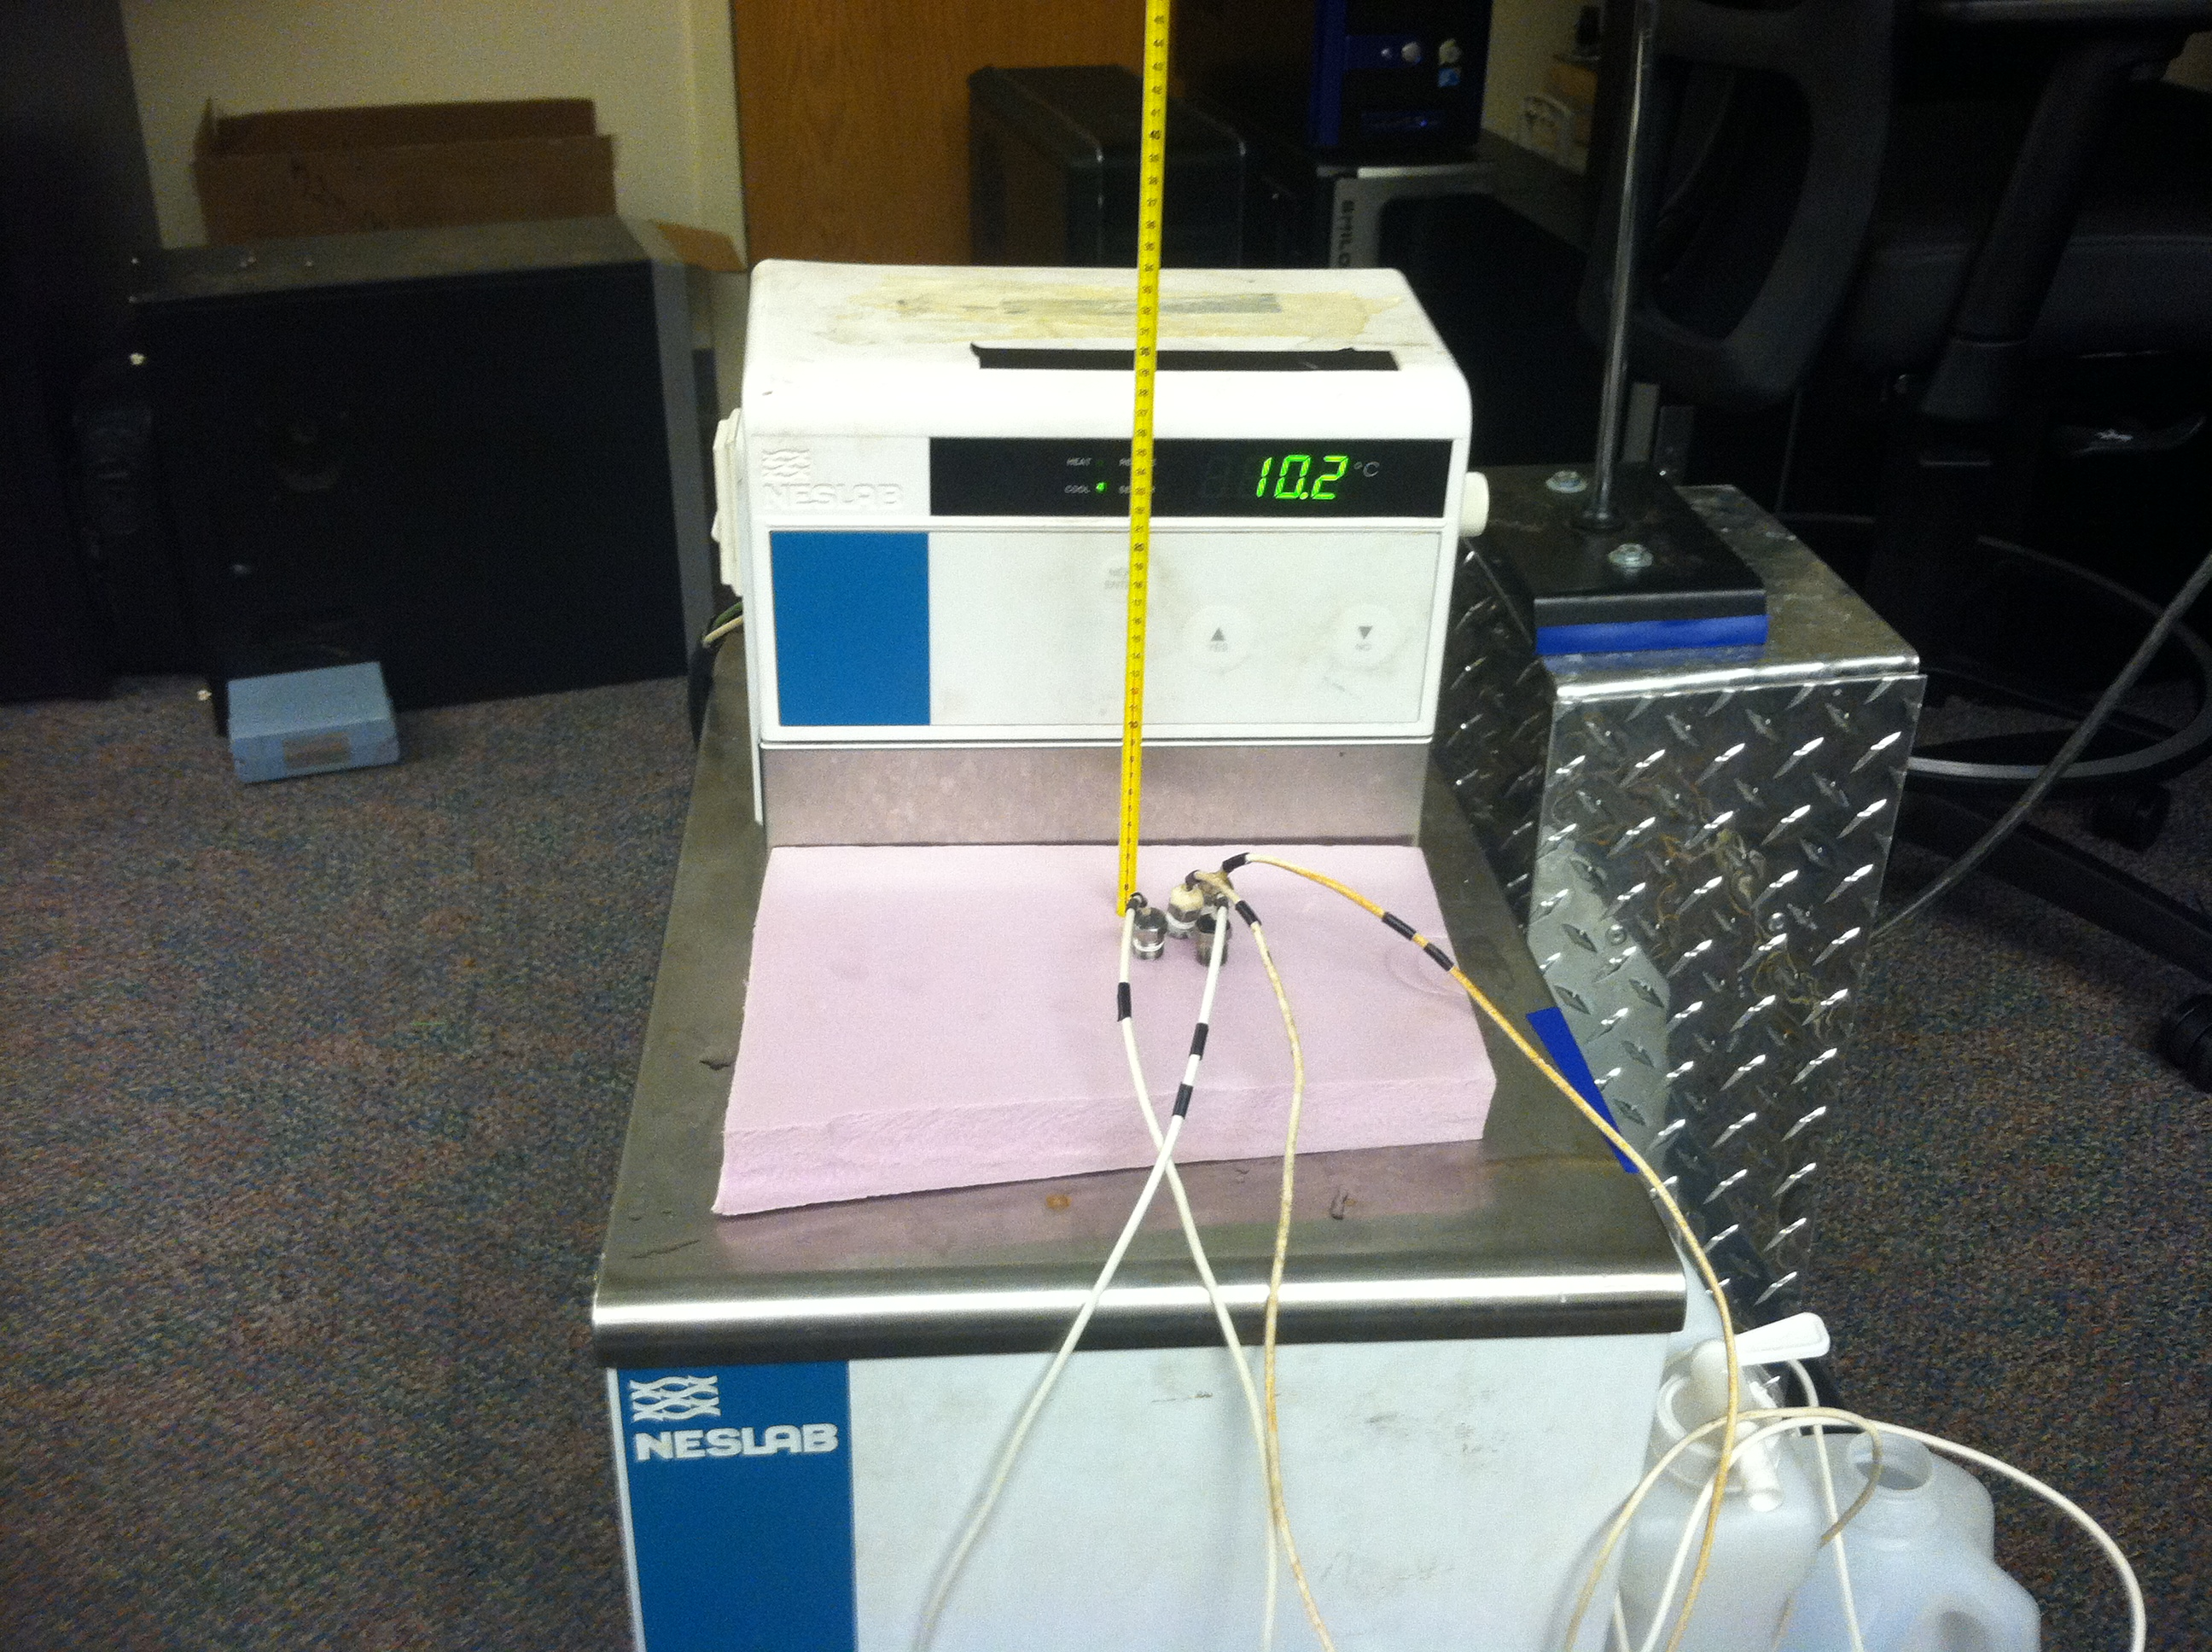
\includegraphics[width=0.8\textwidth]{CalBath.jpg}
	\caption[Calibration bath]{Calibration bath used to calibrate thermistors}
	\label{fig:ExpMethod:Instr:TempCal:CalBath}
\end{figure}

To record the resistance readings, a Fluke Hydra Series II data logger was used to measure the resistance of the thermistor. The data logger's operation manual states that its resistance measurment accuracy is within 0.0125\%. Data logger accuracy when sampling analog signals in the 0-30 VDC range is 0.041\%.

\begin{figure}
	\centering
	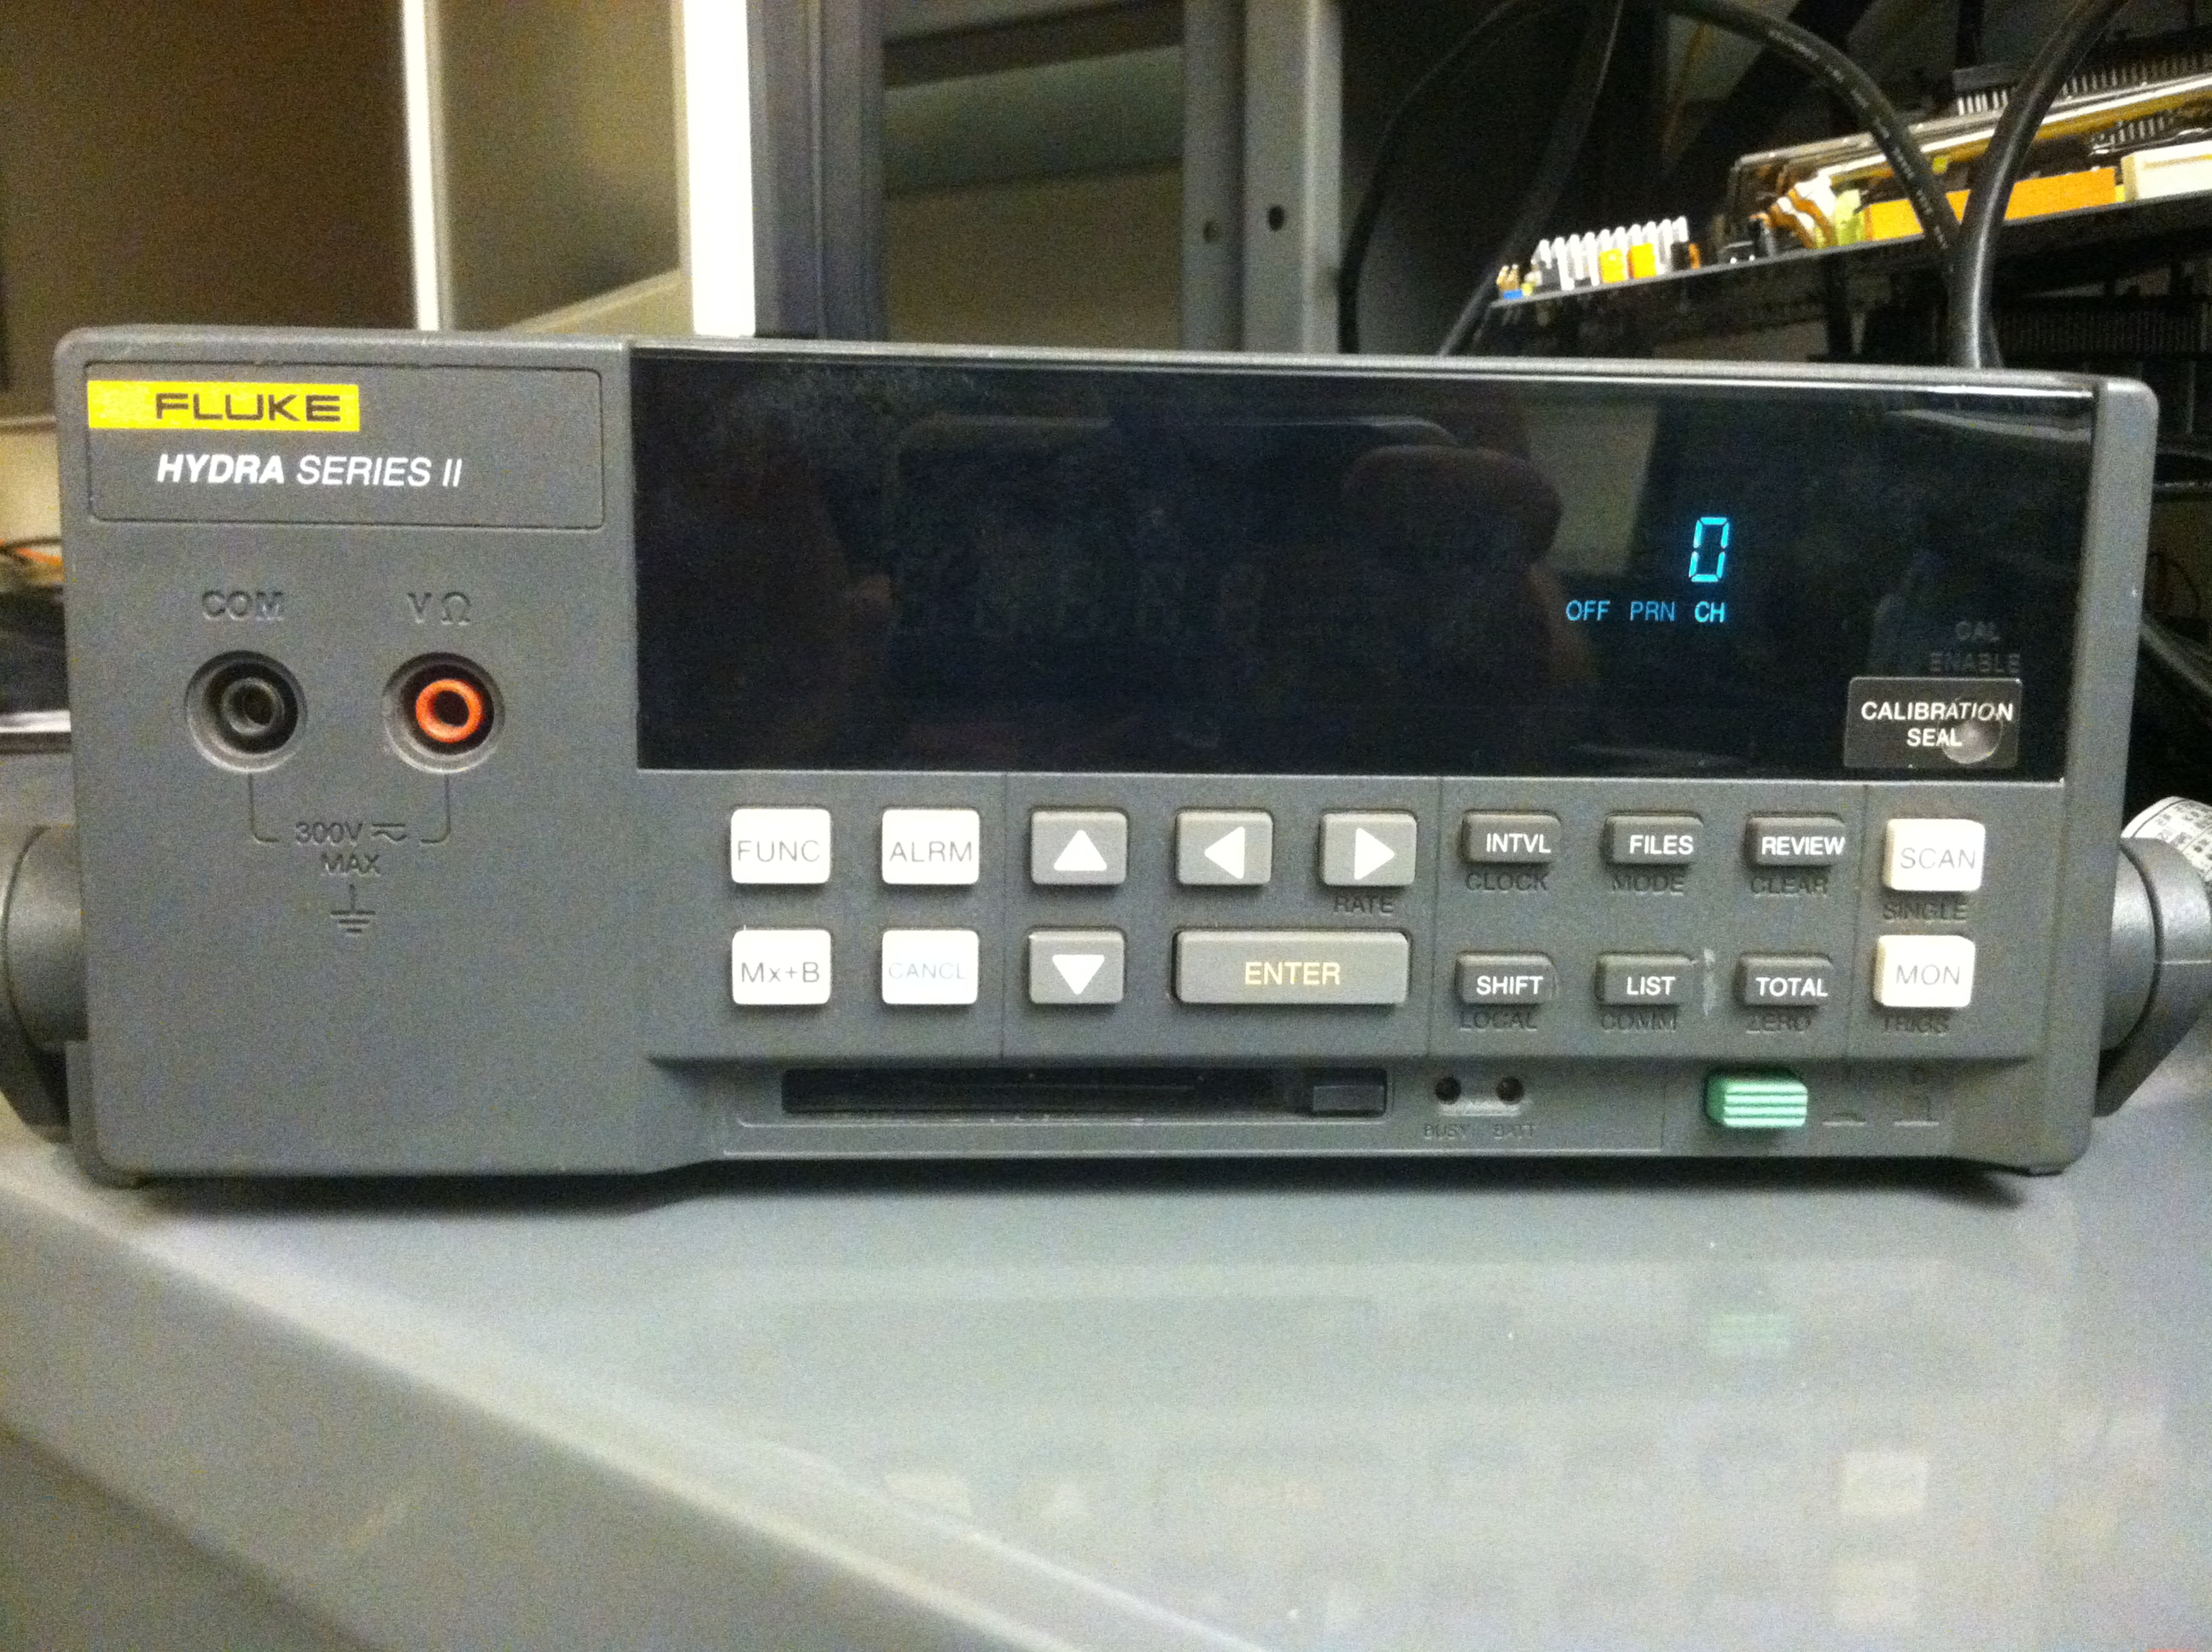
\includegraphics[width=0.8\textwidth]{Fluke.jpg}
	\caption[Fluke data logger]{Fluke data logger used to measure and record flow and temperature measurements}
	\label{fig:ExpMethod:Instr:TempCal:Fluke}
\end{figure}

As an example calibration, the values in Table \ref{tab:ExpMethod:Instr:TempCal:CalData} were taken from a calibration performed on one of the thermistors used in the experiment. From this data, Equation \ref{eq:ExpMethod:Instr:TempCal:SteinhartHart} \citep{SteinhartHart1968} was used to correlate the data.

\begin{table}[h]
	\centering
	\caption{Reference temperature and resistance data from thermistor calibration}
	\label{tab:ExpMethod:Instr:TempCal:CalData}
	\begin{tabular}{c | c}
	\hline
	Ref.\ Temp.\ & Resistance \\
	\hline
	$^\circ$F ($^\circ$C) & Ohms $\Omega$\\
	\hline\hline
	40.82 (4.90) & 5590.54 \\
	\hline
	49.91 (9.95) & 4410.50 \\
	\hline
	59.00 (15.00) & 3492.99 \\
	\hline
	68.00 (20.00) & 2788.47 \\
	\hline
	76.91 (24.95) & 2245.31 \\
	\hline
	85.91 (29.95) & 1815.22 \\
	\hline
	94.91 (34.95) & 1484.24 \\
	\hline
	104.00 (40.00) & 1213.29 \\
	\hline
	113.09 (45.05) & 998.45 \\
	\hline
	122.09 (50.05) & 825.90 \\
	\hline
	\end{tabular}
\end{table}

\begin{equation}
	\frac{1}{T_{abs}} = A + B \cdot ln(\Omega) + C \cdot ln(\Omega)^2 + D \cdot ln(\Omega)^3
	\label{eq:ExpMethod:Instr:TempCal:SteinhartHart}
\end{equation}

Once the data had been correlated, the measured and correlated temperatures were compared to determine the accuracy of the temperature correlation. The correlation coefficients for the data set shown in Table \ref{tab:ExpMethod:Instr:TempCal:CalData} can be seen in Table \ref{tab:ExpMethod:Instr:TempCal:Coefficients}.

\begin{table}[h]
	\centering
	\caption{Correlation coefficients for data in Table \ref{tab:ExpMethod:Instr:TempCal:CalData}}
	\label{tab:ExpMethod:Instr:TempCal:Coefficients}
	\begin{tabular}{c|c|c|c}
	\hline
	A & B & C & D \\
	\hline
	$1.22030 \cdot 10^{-3}$ & $3.25326 \cdot 10^{-4}$ & $-1.08026 \cdot 10^{-5}$ & $5.80588 \cdot 10^{-7}$ \\
	\hline
	\end{tabular}
\end{table}

From Table \ref{tab:ExpMethod:Instr:TempCal:CalDataCompare}, we can see that calibration yielded a good fit to the measured resistance and temperature data. The largest absolute error for this data set is 0.11$^\circ$F (0.06$^\circ$C) which occurred at a temperature measurement near 86$^\circ$F (30$^\circ$C). The rest of the measured values for this particular data set are shown to have absolute temperature errors of around half of the absolute error that occurred at 86$^\circ$F (30$^\circ$C).

\begin{table}[h]
	\centering
	\caption{Measured and correlated temperature for a thermistor calibration}
	\label{tab:ExpMethod:Instr:TempCal:CalDataCompare}
	\begin{tabular}{c | c | c}
	\hline
	$T_{meas}$\ & $T_{corr}$ & $|T_{meas} - T_{corr}|$ \\
	\hline
	$^\circ$F ($^\circ$C) & $^\circ$F ($^\circ$C) & $^\circ$F ($^\circ$C)\\
	\hline\hline
	40.82 (4.90) & 40.86 (4.92) & 0.04 (0.02) \\
	\hline
	49.91 (9.95) & 49.86 (9.92) & 0.05 (0.03) \\
	\hline
	59.00 (15.00) & 58.95 (14.97) & 0.05 (0.03) \\
	\hline
	68.00 (20.00) & 68.00 (20.00) &  0.00 (0.00) \\
	\hline
	76.91 (24.95) & 76.96 (24.98) & 0.05 (0.03) \\
	\hline
	85.91 (29.95) & 86.02 (30.01) & \color{red}{0.11 (0.06)} \\
	\hline
	94.91 (34.95) & 94.87 (34.92) & 0.04 (0.03) \\
	\hline
	104.00 (40.00) & 103.95 (39.97) & 0.05 (0.03) \\
	\hline
	113.09 (45.05) & 113.02 (45.01) & 0.07 (0.04) \\
	\hline
	122.09 (50.05) & 122.14 (50.08) & 0.05 (0.03) \\
	\hline
	\end{tabular}
\end{table}

This result from the previous thermistor cailbration example is typical for all thermistors calibrated. To be conservative, and to simplify the temperature uncertainty analysis, the measured temperature uncertainty for all thermistors was taken to be 0.18$^\circ$F (0.1$^\circ$C). This simplifies the book keeping for the uncertainty analysis and applies a conservative estimate to the error that can be expected from the temperature measurements.

	\subsection{Flow Measurement}
	\label{subsec:ExpMethod:Instr:Flow}

Two separate flow meters were used to measure the circulating fluid flow rate. The first flow meter was manufactured by Omega Engineering with a model number of FTB4605. This flow meter has capability to measure flow from 0.5-20 gpm (1.9-75.7 L/min) with a stated accuracy of $\pm$1.5\%. The flow meter is a pulse output flow meter, and therefore it requires a signal conditioner to convert the pulse output to an analog signal for the data logger to record. The signal conditioner was also purchased from Omega Engineering with a model number of DFP701. The Omega flow meter was used for all pond heat rejection tests.

The second flow meter was purchased from Gem Sensors. Its model number is 230216 and is stated by the manufacture to have an accuracy of $\pm$ 7\%. The flow meter has a flow range from 0.5-12 gpm (1.9-45.4 L/min) and outputs an analog signal. A photo of this flow meter during a heat extraction test can be seen in Figure \ref{fig:ExpMethod:Instr:Flow:GemFlowMeter}.

\begin{figure}
	\centering
	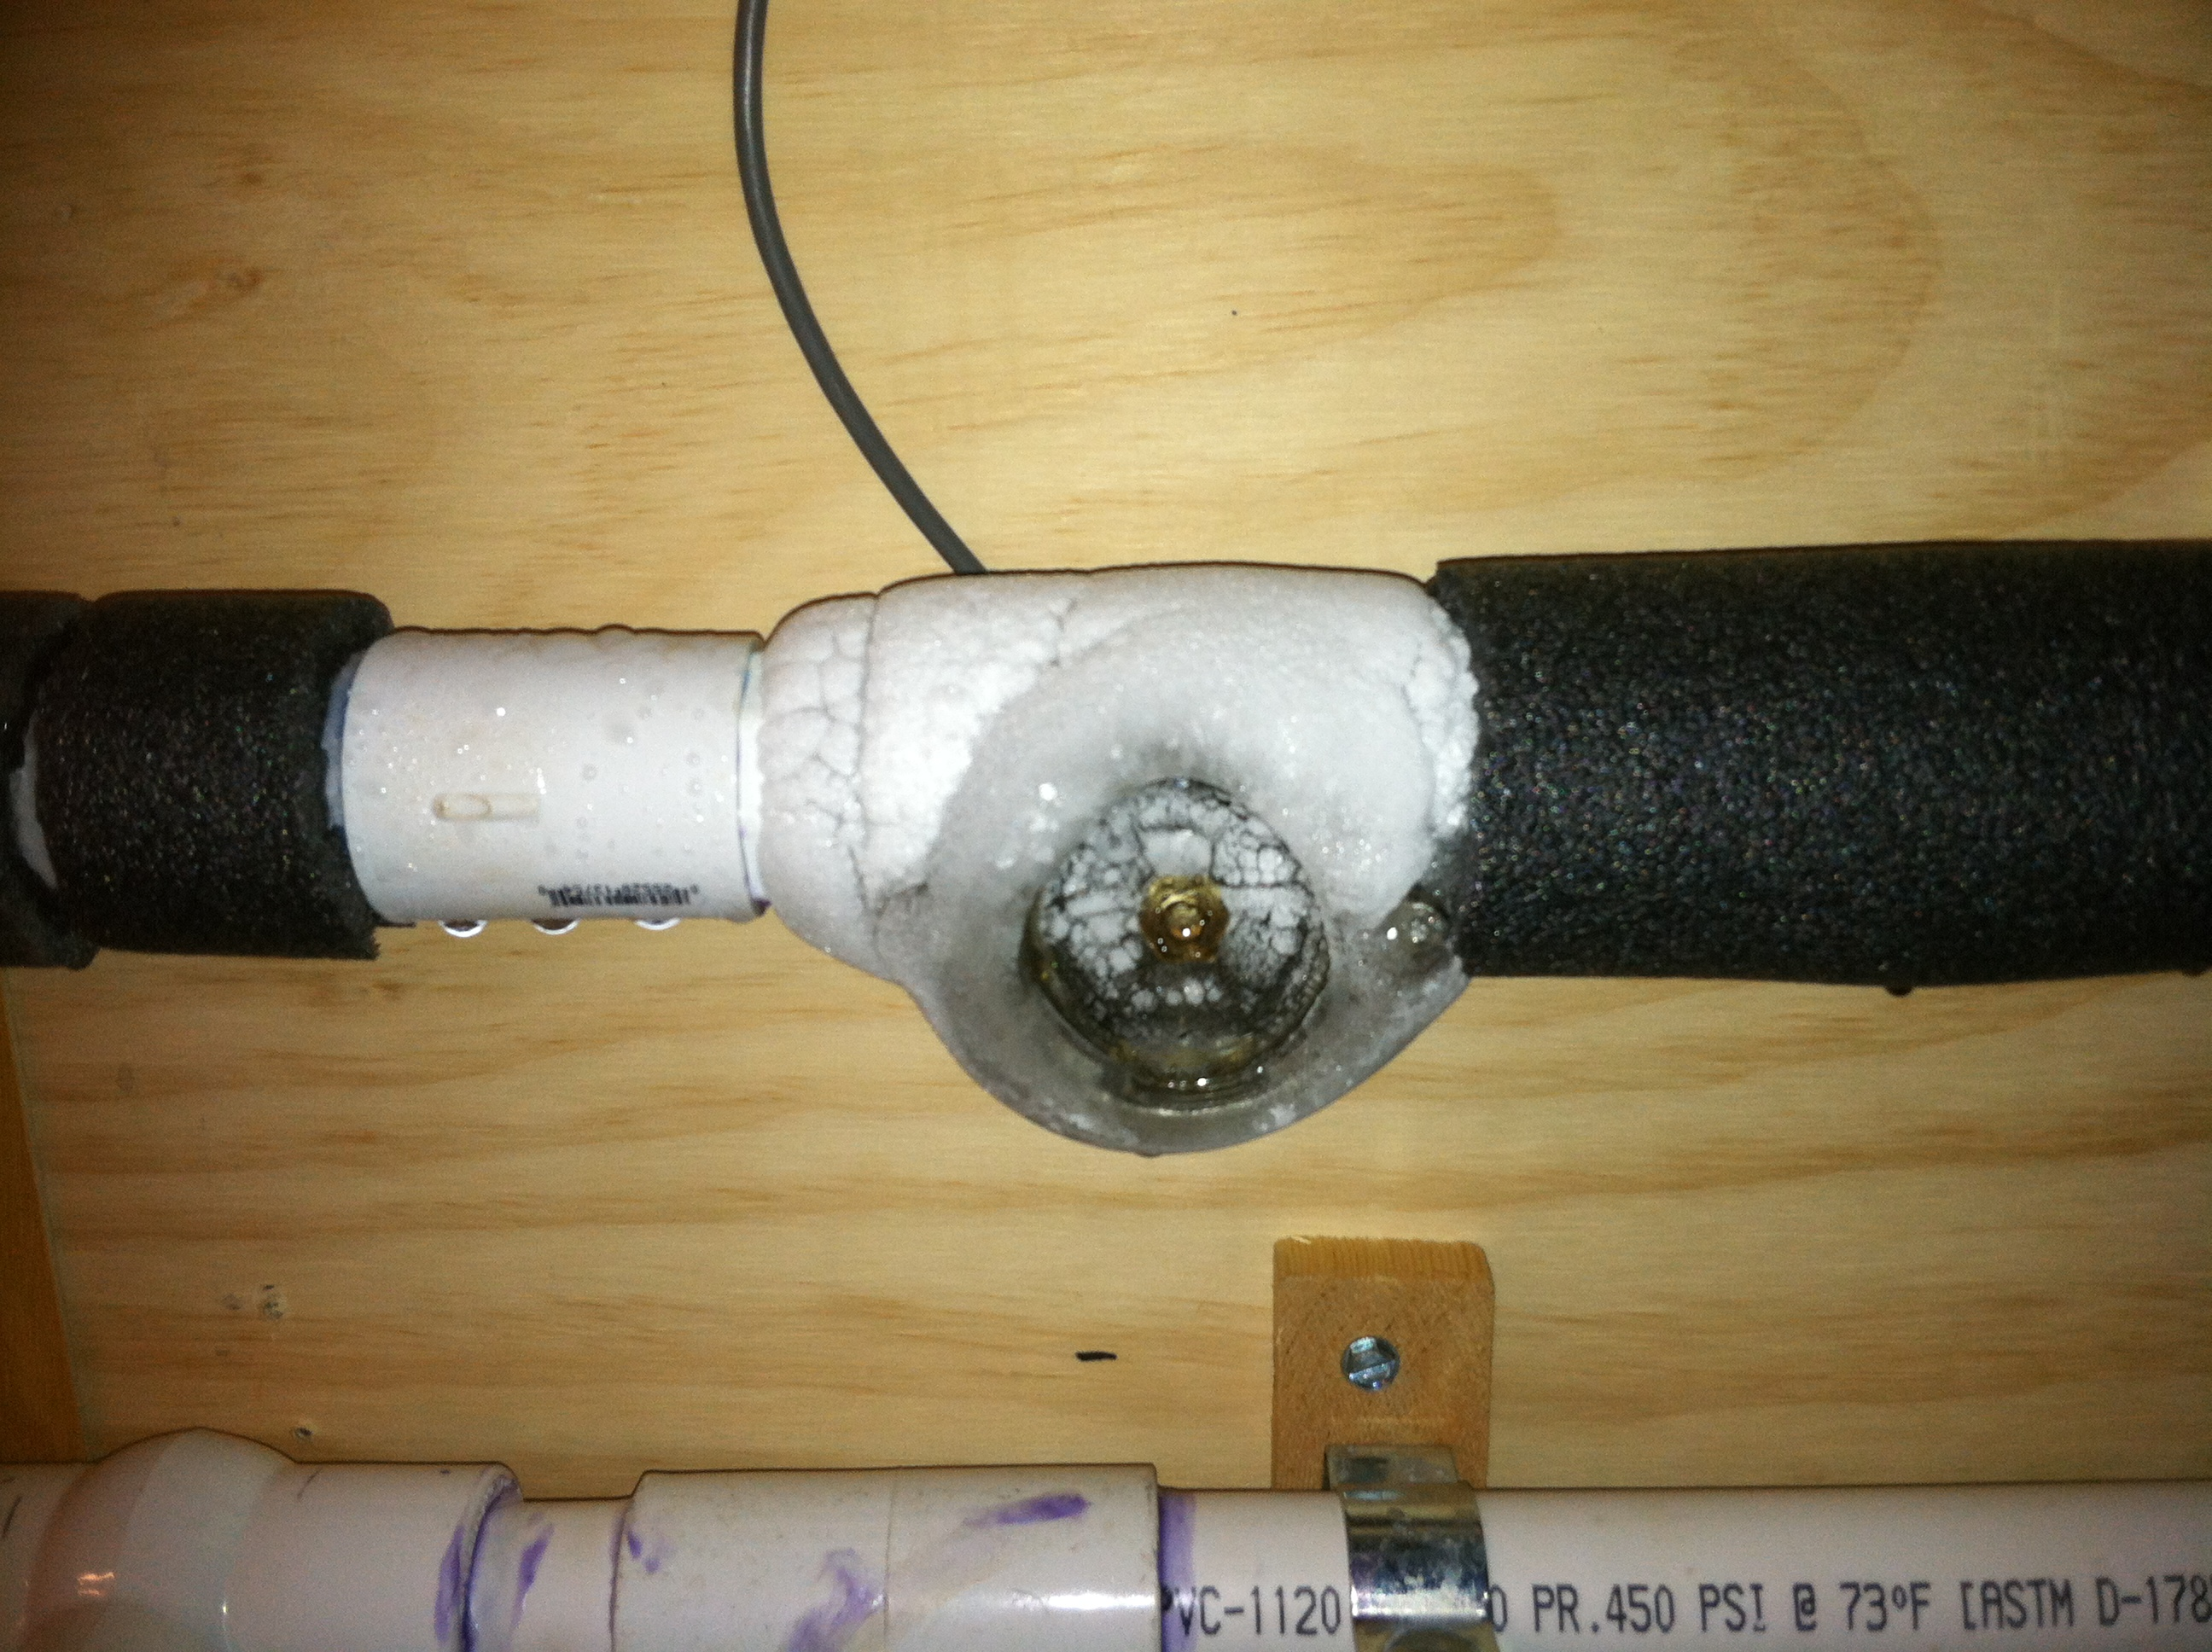
\includegraphics[width=0.8\textwidth]{GemFlowMeter.jpg}
	\caption[Gem flow meter]{Gem flow meter during heat extraction test}
	\label{fig:ExpMethod:Instr:Flow:GemFlowMeter}
\end{figure}

	\subsection{Flow Measurement Calibration}
	\label{subsec:ExpMethod:Instr:FlowCal}

To calibrate the flow meters, three 5 gal.\ (18.9 L) buckets, a stopwatch, and scale calibrated to 0.11 lb (0.05 kg) were used. To determine the flow rate, the flow through the flow meter was set to run at steady state conditions. Fluid was then sampled from the flow stream using the buckets and the total time the fluid was sampled was recorded. The mass of the fluid was determined by subtracting the initial weight of each bucket, and the total fluid mass for a specific flow rate was then determined. Once the fluid was sample from the flow stream, it was returned to the purge tank feeding the pump and flow meter.

This information was then used to calculate the volumetric flow rate for that particular fluid flow set point. The data logger was also used to record the analog signal at 5 sec.\ intervals. The average analog voltage during the flow measurement was then taken as the flow meter output for that set point. Because the fluid is essentially flowing in a closed loop and no heat is being added, the fluid temperature was sampled once during the calibration process. This temperature was necessary to determine the density of the circulating fluid.

Table \ref{tab:ExpMethod:Instr:FlowCal:CalDataCompare} shows data taken from a calibration of the Gem flow meter. The maximum absolute percent error for the Gem flow meter is 1.46\% with an error standard deviation of 0.084 gpm (0.32 L/min). The Omega flow meter was calibrated in the same manner and shows a maximum absolute percent error of 0.6\% with an error standard deviation of 0.015 gpm (0.06 L/min). Because two times the standard deviation represents the 95\% confidence interval, two times the standard deviation is what flow measurement uncertainty was taken as.

\begin{table}[h]
	\centering
	\caption{Measured and correlated flow rates for Gem flow meter}
	\label{tab:ExpMethod:Instr:FlowCal:CalDataCompare}
	\begin{tabular}{c | c | c | c | c}
	\hline
	FM Output & $\dot{V}_{meas}$\ & $\dot{V}_{corr}$ & $|\dot{V}_{meas} - \dot{V}_{corr}|$ & \% Error\\
	\hline
	VDC & gpm (L/min) & gpm (L/min) & gpm (L/min)\\
	\hline\hline
	0.02 & 0.000 (0.0) & 0.091 (0.34) & 0.091 (0.34) & - \\
	\hline
	2.91 & 5.903 (22.35) & 5.935 (22.47) & 0.032 (0.12) & 0.55\\
	\hline
	2.93 & 6.049 (22.90) & 5.965 (22.58) & 0.085 (0.32) & -1.40 \\
	\hline
	3.50 & 7.227 (27.36) & 7.125 (26.97) & 0.102 (0.39) & -1.41 \\
	\hline
	3.53 & 7.221 (27.33) & 7.188 (27.21) & 0.033 (0.12) & -0.45\\
	\hline
	4.33 & 8.852 (33.51) & 8.799 (33.31) & 0.053 (0.20) & -0.59\\
	\hline
	4.33 & 8.831 (33.43) & 8.801 (33.32) & 0.030 (0.11) & -0.34\\
	\hline
	5.31 & 10.77 (40.77) & 10.79 (40.84) & 0.021 (0.08) & 0.19\\
	\hline
	5.38 & 10.77 (40.77) & 10.93 (41.37) & 0.157 (0.59) & \color{red}{1.46} \\
	\hline
	\end{tabular}
\end{table}

	\subsection{Other Instrumentation}
	\label{subsec:ExpMethod:Instr:Other}

Instrumentation used in these experiments apart from the temperature sensors, flow meters, and data loggers, are the load cells which were purchased through Interface Inc. The first set of load cells were submersible and had a total capacity of 500 lb (2,224 N) in tension or compression. The submersible load cells had a model number of 2420BTH-500. A photo of one of these load cells can be seen in Figure \ref{fig:ExpMethod:HeatExtr:Apparatus:UWLoadCell}.

The second set of load cells were also purchased from Interface. These load cells were tension only load cells with a tensile capacity of 500 lb (2,224 N). A photo of one of these load cells can be seen in Figure \ref{fig:ExpMethod:HeatExtr:Apparatus:TensionLoadCell}.

All load cell outputs were processed through a signal conditioning unit (model SGA). This signal conditioner aggregated the output signals from the three load cells and amplified the output to an 0-10 VDC analog signal. Load cells came pre-calibrated from Interface.
